\documentclass[twoside]{book}

% Packages required by doxygen
\usepackage{fixltx2e}
\usepackage{calc}
\usepackage{doxygen}
\usepackage[export]{adjustbox} % also loads graphicx
\usepackage{graphicx}
\usepackage[utf8]{inputenc}
\usepackage{makeidx}
\usepackage{multicol}
\usepackage{multirow}
\PassOptionsToPackage{warn}{textcomp}
\usepackage{textcomp}
\usepackage[nointegrals]{wasysym}
\usepackage[table]{xcolor}

% Font selection
\usepackage[T1]{fontenc}
\usepackage[scaled=.90]{helvet}
\usepackage{courier}
\usepackage{amssymb}
\usepackage{sectsty}
\renewcommand{\familydefault}{\sfdefault}
\allsectionsfont{%
  \fontseries{bc}\selectfont%
  \color{darkgray}%
}
\renewcommand{\DoxyLabelFont}{%
  \fontseries{bc}\selectfont%
  \color{darkgray}%
}
\newcommand{\+}{\discretionary{\mbox{\scriptsize$\hookleftarrow$}}{}{}}

% Page & text layout
\usepackage{geometry}
\geometry{%
  a4paper,%
  top=2.5cm,%
  bottom=2.5cm,%
  left=2.5cm,%
  right=2.5cm%
}
\tolerance=750
\hfuzz=15pt
\hbadness=750
\setlength{\emergencystretch}{15pt}
\setlength{\parindent}{0cm}
\setlength{\parskip}{3ex plus 2ex minus 2ex}
\makeatletter
\renewcommand{\paragraph}{%
  \@startsection{paragraph}{4}{0ex}{-1.0ex}{1.0ex}{%
    \normalfont\normalsize\bfseries\SS@parafont%
  }%
}
\renewcommand{\subparagraph}{%
  \@startsection{subparagraph}{5}{0ex}{-1.0ex}{1.0ex}{%
    \normalfont\normalsize\bfseries\SS@subparafont%
  }%
}
\makeatother

% Headers & footers
\usepackage{fancyhdr}
\pagestyle{fancyplain}
\fancyhead[LE]{\fancyplain{}{\bfseries\thepage}}
\fancyhead[CE]{\fancyplain{}{}}
\fancyhead[RE]{\fancyplain{}{\bfseries\leftmark}}
\fancyhead[LO]{\fancyplain{}{\bfseries\rightmark}}
\fancyhead[CO]{\fancyplain{}{}}
\fancyhead[RO]{\fancyplain{}{\bfseries\thepage}}
\fancyfoot[LE]{\fancyplain{}{}}
\fancyfoot[CE]{\fancyplain{}{}}
\fancyfoot[RE]{\fancyplain{}{\bfseries\scriptsize Generated by Doxygen }}
\fancyfoot[LO]{\fancyplain{}{\bfseries\scriptsize Generated by Doxygen }}
\fancyfoot[CO]{\fancyplain{}{}}
\fancyfoot[RO]{\fancyplain{}{}}
\renewcommand{\footrulewidth}{0.4pt}
\renewcommand{\chaptermark}[1]{%
  \markboth{#1}{}%
}
\renewcommand{\sectionmark}[1]{%
  \markright{\thesection\ #1}%
}

% Indices & bibliography
\usepackage{natbib}
\usepackage[titles]{tocloft}
\setcounter{tocdepth}{3}
\setcounter{secnumdepth}{5}
\makeindex

% Hyperlinks (required, but should be loaded last)
\usepackage{ifpdf}
\ifpdf
  \usepackage[pdftex,pagebackref=true]{hyperref}
\else
  \usepackage[ps2pdf,pagebackref=true]{hyperref}
\fi
\hypersetup{%
  colorlinks=true,%
  linkcolor=blue,%
  citecolor=blue,%
  unicode%
}

% Custom commands
\newcommand{\clearemptydoublepage}{%
  \newpage{\pagestyle{empty}\cleardoublepage}%
}

\usepackage{caption}
\captionsetup{labelsep=space,justification=centering,font={bf},singlelinecheck=off,skip=4pt,position=top}

%===== C O N T E N T S =====

\begin{document}

% Titlepage & ToC
\hypersetup{pageanchor=false,
             bookmarksnumbered=true,
             pdfencoding=unicode
            }
\pagenumbering{alph}
\begin{titlepage}
\vspace*{7cm}
\begin{center}%
{\Large Hexgame \\[1ex]\large 0.\+0.\+1 }\\
\vspace*{1cm}
{\large Generated by Doxygen 1.8.13}\\
\end{center}
\end{titlepage}
\clearemptydoublepage
\pagenumbering{roman}
\tableofcontents
\clearemptydoublepage
\pagenumbering{arabic}
\hypersetup{pageanchor=true}

%--- Begin generated contents ---
\chapter{Hierarchical Index}
\section{Class Hierarchy}
This inheritance list is sorted roughly, but not completely, alphabetically\+:\begin{DoxyCompactList}
\item \contentsline{section}{Color}{\pageref{structColor}}{}
\item \contentsline{section}{Field}{\pageref{classField}}{}
\item \contentsline{section}{Figure}{\pageref{classFigure}}{}
\begin{DoxyCompactList}
\item \contentsline{section}{Bush}{\pageref{classBush}}{}
\item \contentsline{section}{Coin}{\pageref{classCoin}}{}
\item \contentsline{section}{Player}{\pageref{classPlayer}}{}
\end{DoxyCompactList}
\item \contentsline{section}{Game}{\pageref{classGame}}{}
\item \contentsline{section}{Tile}{\pageref{classTile}}{}
\item \contentsline{section}{vec2}{\pageref{structvec2}}{}
\end{DoxyCompactList}

\chapter{Class Index}
\section{Class List}
Here are the classes, structs, unions and interfaces with brief descriptions\+:\begin{DoxyCompactList}
\item\contentsline{section}{\hyperlink{classBush}{Bush} }{\pageref{classBush}}{}
\item\contentsline{section}{\hyperlink{classCoin}{Coin} }{\pageref{classCoin}}{}
\item\contentsline{section}{\hyperlink{structColor}{Color} }{\pageref{structColor}}{}
\item\contentsline{section}{\hyperlink{classField}{Field} }{\pageref{classField}}{}
\item\contentsline{section}{\hyperlink{classFigure}{Figure} }{\pageref{classFigure}}{}
\item\contentsline{section}{\hyperlink{classGame}{Game} }{\pageref{classGame}}{}
\item\contentsline{section}{\hyperlink{classPlayer}{Player} }{\pageref{classPlayer}}{}
\item\contentsline{section}{\hyperlink{classTile}{Tile} }{\pageref{classTile}}{}
\item\contentsline{section}{\hyperlink{structvec2}{vec2} }{\pageref{structvec2}}{}
\end{DoxyCompactList}

\chapter{File Index}
\section{File List}
Here is a list of all files with brief descriptions\+:\begin{DoxyCompactList}
\item\contentsline{section}{\hyperlink{bush_8h}{bush.\+h} }{\pageref{bush_8h}}{}
\item\contentsline{section}{\hyperlink{coin_8h}{coin.\+h} }{\pageref{coin_8h}}{}
\item\contentsline{section}{\hyperlink{color_8h}{color.\+h} }{\pageref{color_8h}}{}
\item\contentsline{section}{\hyperlink{constants_8h}{constants.\+h} }{\pageref{constants_8h}}{}
\item\contentsline{section}{\hyperlink{field_8cpp}{field.\+cpp} }{\pageref{field_8cpp}}{}
\item\contentsline{section}{\hyperlink{field_8h}{field.\+h} }{\pageref{field_8h}}{}
\item\contentsline{section}{\hyperlink{figure_8h}{figure.\+h} }{\pageref{figure_8h}}{}
\item\contentsline{section}{\hyperlink{game_8cpp}{game.\+cpp} }{\pageref{game_8cpp}}{}
\item\contentsline{section}{\hyperlink{game_8h}{game.\+h} }{\pageref{game_8h}}{}
\item\contentsline{section}{\hyperlink{player_8cpp}{player.\+cpp} }{\pageref{player_8cpp}}{}
\item\contentsline{section}{\hyperlink{player_8h}{player.\+h} }{\pageref{player_8h}}{}
\item\contentsline{section}{\hyperlink{tile_8cpp}{tile.\+cpp} }{\pageref{tile_8cpp}}{}
\item\contentsline{section}{\hyperlink{tile_8h}{tile.\+h} }{\pageref{tile_8h}}{}
\item\contentsline{section}{\hyperlink{util_8cpp}{util.\+cpp} }{\pageref{util_8cpp}}{}
\item\contentsline{section}{\hyperlink{util_8h}{util.\+h} }{\pageref{util_8h}}{}
\item\contentsline{section}{\hyperlink{vec2_8cpp}{vec2.\+cpp} }{\pageref{vec2_8cpp}}{}
\item\contentsline{section}{\hyperlink{vec2_8h}{vec2.\+h} }{\pageref{vec2_8h}}{}
\end{DoxyCompactList}

\chapter{Class Documentation}
\hypertarget{classBush}{}\section{Bush Class Reference}
\label{classBush}\index{Bush@{Bush}}


{\ttfamily \#include $<$bush.\+h$>$}



Inheritance diagram for Bush\+:
\nopagebreak
\begin{figure}[H]
\begin{center}
\leavevmode
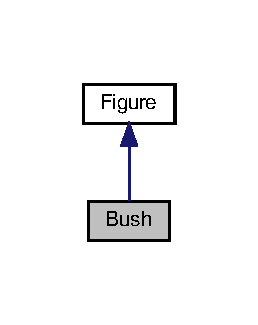
\includegraphics[width=124pt]{d3/d66/classBush__inherit__graph}
\end{center}
\end{figure}


Collaboration diagram for Bush\+:
\nopagebreak
\begin{figure}[H]
\begin{center}
\leavevmode
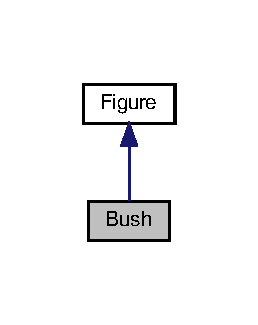
\includegraphics[width=124pt]{dd/d5d/classBush__coll__graph}
\end{center}
\end{figure}
\subsection*{Public Member Functions}
\begin{DoxyCompactItemize}
\item 
void \hyperlink{classBush_aa73b14744dbe2b868142dc2deae485ba}{draw} (\hyperlink{structvec2}{vec2} position) const
\end{DoxyCompactItemize}


\subsection{Member Function Documentation}
\mbox{\Hypertarget{classBush_aa73b14744dbe2b868142dc2deae485ba}\label{classBush_aa73b14744dbe2b868142dc2deae485ba}} 
\index{Bush@{Bush}!draw@{draw}}
\index{draw@{draw}!Bush@{Bush}}
\subsubsection{\texorpdfstring{draw()}{draw()}}
{\footnotesize\ttfamily void Bush\+::draw (\begin{DoxyParamCaption}\item[{\hyperlink{structvec2}{vec2}}]{position }\end{DoxyParamCaption}) const\hspace{0.3cm}{\ttfamily [inline]}, {\ttfamily [virtual]}}



Implements \hyperlink{classFigure_ac16583e764bdc244076957bf775e4866}{Figure}.



The documentation for this class was generated from the following file\+:\begin{DoxyCompactItemize}
\item 
\hyperlink{bush_8h}{bush.\+h}\end{DoxyCompactItemize}

\hypertarget{classCoin}{}\section{Coin Class Reference}
\label{classCoin}\index{Coin@{Coin}}


{\ttfamily \#include $<$coin.\+h$>$}



Inheritance diagram for Coin\+:
\nopagebreak
\begin{figure}[H]
\begin{center}
\leavevmode
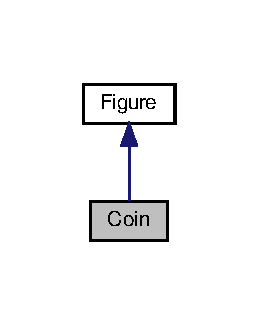
\includegraphics[width=124pt]{dc/d38/classCoin__inherit__graph}
\end{center}
\end{figure}


Collaboration diagram for Coin\+:
\nopagebreak
\begin{figure}[H]
\begin{center}
\leavevmode
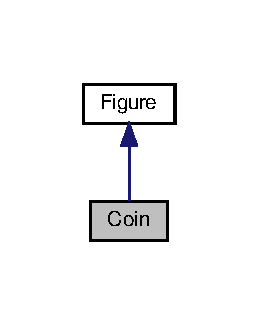
\includegraphics[width=124pt]{d7/de3/classCoin__coll__graph}
\end{center}
\end{figure}
\subsection*{Public Member Functions}
\begin{DoxyCompactItemize}
\item 
void \hyperlink{classCoin_a13812f35d85e19553fe36350c947204c}{draw} (\hyperlink{structvec2}{vec2} position) const
\end{DoxyCompactItemize}


\subsection{Member Function Documentation}
\mbox{\Hypertarget{classCoin_a13812f35d85e19553fe36350c947204c}\label{classCoin_a13812f35d85e19553fe36350c947204c}} 
\index{Coin@{Coin}!draw@{draw}}
\index{draw@{draw}!Coin@{Coin}}
\subsubsection{\texorpdfstring{draw()}{draw()}}
{\footnotesize\ttfamily void Coin\+::draw (\begin{DoxyParamCaption}\item[{\hyperlink{structvec2}{vec2}}]{position }\end{DoxyParamCaption}) const\hspace{0.3cm}{\ttfamily [inline]}, {\ttfamily [virtual]}}



Implements \hyperlink{classFigure_ac16583e764bdc244076957bf775e4866}{Figure}.



The documentation for this class was generated from the following file\+:\begin{DoxyCompactItemize}
\item 
\hyperlink{coin_8h}{coin.\+h}\end{DoxyCompactItemize}

\hypertarget{structColor}{}\section{Color Struct Reference}
\label{structColor}\index{Color@{Color}}


{\ttfamily \#include $<$color.\+h$>$}

\subsection*{Public Member Functions}
\begin{DoxyCompactItemize}
\item 
\hyperlink{structColor_a9a742cbe9f9f4037f5d9f4e81a9b2428}{Color} ()
\item 
\hyperlink{structColor_ad999a91996687a8593bd646ae9a9dbbf}{Color} (unsigned char \+\_\+red, unsigned char \+\_\+green, unsigned char \+\_\+blue)
\item 
const \hyperlink{structColor}{Color} \& \hyperlink{structColor_ad16157e8a956c472eab89137edde458a}{operator=} (const \hyperlink{structColor}{Color} \&color)
\end{DoxyCompactItemize}
\subsection*{Public Attributes}
\begin{DoxyCompactItemize}
\item 
unsigned char \hyperlink{structColor_a245f5a423cdaaaeff27047036c24b7ef}{red}
\item 
unsigned char \hyperlink{structColor_a070831365fe6c626bc0020915a917081}{green}
\item 
unsigned char \hyperlink{structColor_a5b425af958edb0e7835eb08daeb90e71}{blue}
\end{DoxyCompactItemize}


\subsection{Constructor \& Destructor Documentation}
\mbox{\Hypertarget{structColor_a9a742cbe9f9f4037f5d9f4e81a9b2428}\label{structColor_a9a742cbe9f9f4037f5d9f4e81a9b2428}} 
\index{Color@{Color}!Color@{Color}}
\index{Color@{Color}!Color@{Color}}
\subsubsection{\texorpdfstring{Color()}{Color()}\hspace{0.1cm}{\footnotesize\ttfamily [1/2]}}
{\footnotesize\ttfamily Color\+::\+Color (\begin{DoxyParamCaption}{ }\end{DoxyParamCaption})\hspace{0.3cm}{\ttfamily [inline]}}

\mbox{\Hypertarget{structColor_ad999a91996687a8593bd646ae9a9dbbf}\label{structColor_ad999a91996687a8593bd646ae9a9dbbf}} 
\index{Color@{Color}!Color@{Color}}
\index{Color@{Color}!Color@{Color}}
\subsubsection{\texorpdfstring{Color()}{Color()}\hspace{0.1cm}{\footnotesize\ttfamily [2/2]}}
{\footnotesize\ttfamily Color\+::\+Color (\begin{DoxyParamCaption}\item[{unsigned char}]{\+\_\+red,  }\item[{unsigned char}]{\+\_\+green,  }\item[{unsigned char}]{\+\_\+blue }\end{DoxyParamCaption})\hspace{0.3cm}{\ttfamily [inline]}}



\subsection{Member Function Documentation}
\mbox{\Hypertarget{structColor_ad16157e8a956c472eab89137edde458a}\label{structColor_ad16157e8a956c472eab89137edde458a}} 
\index{Color@{Color}!operator=@{operator=}}
\index{operator=@{operator=}!Color@{Color}}
\subsubsection{\texorpdfstring{operator=()}{operator=()}}
{\footnotesize\ttfamily const \hyperlink{structColor}{Color}\& Color\+::operator= (\begin{DoxyParamCaption}\item[{const \hyperlink{structColor}{Color} \&}]{color }\end{DoxyParamCaption})\hspace{0.3cm}{\ttfamily [inline]}}



\subsection{Member Data Documentation}
\mbox{\Hypertarget{structColor_a5b425af958edb0e7835eb08daeb90e71}\label{structColor_a5b425af958edb0e7835eb08daeb90e71}} 
\index{Color@{Color}!blue@{blue}}
\index{blue@{blue}!Color@{Color}}
\subsubsection{\texorpdfstring{blue}{blue}}
{\footnotesize\ttfamily unsigned char Color\+::blue}

\mbox{\Hypertarget{structColor_a070831365fe6c626bc0020915a917081}\label{structColor_a070831365fe6c626bc0020915a917081}} 
\index{Color@{Color}!green@{green}}
\index{green@{green}!Color@{Color}}
\subsubsection{\texorpdfstring{green}{green}}
{\footnotesize\ttfamily unsigned char Color\+::green}

\mbox{\Hypertarget{structColor_a245f5a423cdaaaeff27047036c24b7ef}\label{structColor_a245f5a423cdaaaeff27047036c24b7ef}} 
\index{Color@{Color}!red@{red}}
\index{red@{red}!Color@{Color}}
\subsubsection{\texorpdfstring{red}{red}}
{\footnotesize\ttfamily unsigned char Color\+::red}



The documentation for this struct was generated from the following file\+:\begin{DoxyCompactItemize}
\item 
\hyperlink{color_8h}{color.\+h}\end{DoxyCompactItemize}

\hypertarget{classField}{}\section{Field Class Reference}
\label{classField}\index{Field@{Field}}


{\ttfamily \#include $<$field.\+h$>$}



Collaboration diagram for Field\+:
\nopagebreak
\begin{figure}[H]
\begin{center}
\leavevmode
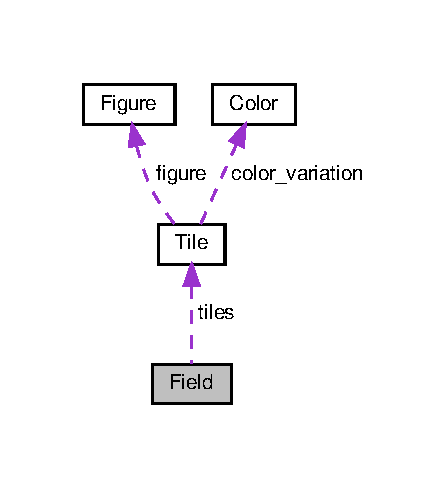
\includegraphics[width=215pt]{d3/d0e/classField__coll__graph}
\end{center}
\end{figure}
\subsection*{Public Member Functions}
\begin{DoxyCompactItemize}
\item 
\hyperlink{classField_ace906b0a3a8057fd29feb3208738da8b}{Field} (unsigned width, unsigned height)
\item 
\hyperlink{classField_a8f32e3182de753297bf48cbf81266fa0}{Field} (unsigned width, unsigned height, unsigned discrepancy, unsigned smoothing)
\item 
\hyperlink{classField_a45d6e6d09b8f8e46de62b40119d62c60}{$\sim$\+Field} ()
\item 
void \hyperlink{classField_a7f7717afdf36e1c572743645215b09ad}{smoothen} (unsigned amount)
\item 
void \hyperlink{classField_ac4e988bd9aa40e2821d43576907abe81}{smoothen} (std\+::vector$<$ \hyperlink{classTile}{Tile} $\ast$$>$ to\+\_\+smooth)
\item 
void \hyperlink{classField_aa4550e9ebc14ccaa6d1e3e110906c9b9}{forestify} (unsigned amount)
\item 
void \hyperlink{classField_a6ba5bccf334f6022710acb5a4bbe5e09}{draw} (\hyperlink{structvec2}{vec2} translation) const
\item 
void \hyperlink{classField_a908ce6baa14bf69944f63caed4032a8a}{mark} (\hyperlink{structvec2}{vec2} translation, std\+::vector$<$ \hyperlink{classTile}{Tile} $\ast$$>$ path) const
\item 
\hyperlink{classTile}{Tile} $\ast$ \hyperlink{classField_aa31d2b14e58becf8741a3b4dc19ecc52}{tile\+\_\+at} (int x, int y) const
\item 
\hyperlink{structvec2}{vec2} \hyperlink{classField_a361bc41ed73bb361ee84c390a9f9c0d0}{get\+Vector\+Position} (\hyperlink{classTile}{Tile} $\ast$pos) const
\item 
\hyperlink{structvec2}{vec2} \hyperlink{classField_aab4e4dfa665fb94c158e1902f1bd46c1}{get\+Drawing\+Position} (\hyperlink{classTile}{Tile} $\ast$pos) const
\item 
\hyperlink{classTile}{Tile} $\ast$ \hyperlink{classField_a8068a7e61bc891b1e4cf7d4d9d7afd12}{estimat\+Tile} (\hyperlink{structvec2}{vec2} pos) const
\item 
std\+::vector$<$ \hyperlink{classTile}{Tile} $\ast$ $>$ \hyperlink{classField_a0e5a676ab734632e575513491f049330}{find\+Path} (\hyperlink{classTile}{Tile} $\ast$start\+\_\+tile, \hyperlink{classTile}{Tile} $\ast$destination\+\_\+tile) const
\item 
std\+::vector$<$ \hyperlink{classTile}{Tile} $\ast$ $>$ \hyperlink{classField_a7bc17bb858f3707e156d1fb6e32a4196}{find\+Surounding} (\hyperlink{classTile}{Tile} $\ast$start\+\_\+tile, int n) const
\item 
std\+::vector$<$ \hyperlink{classTile}{Tile} $\ast$ $>$ \hyperlink{classField_a36a2c3f822ece390f7b69f528d1d8742}{get\+Surounding} (\hyperlink{classTile}{Tile} $\ast$position) const
\item 
float \hyperlink{classField_a1b07030b79bb1e68dbf82aff2bd45730}{heuristic} (\hyperlink{classTile}{Tile} $\ast$start, \hyperlink{classTile}{Tile} $\ast$end) const
\item 
const unsigned $\ast$ \hyperlink{classField_a6daa65acbf49cc9c9516eca76efeaec2}{get\+Size} () const
\end{DoxyCompactItemize}
\subsection*{Static Public Member Functions}
\begin{DoxyCompactItemize}
\item 
static std\+::map$<$ int, \hyperlink{structColor}{Color} $>$ \hyperlink{classField_aeb9f68e86153bfefe2191149fdd840ed}{initialize\+Color\+Map} ()
\end{DoxyCompactItemize}
\subsection*{Private Member Functions}
\begin{DoxyCompactItemize}
\item 
\hyperlink{classField_a72ebbf8a9843cfd7844aa76698ea1541}{Field} (const \hyperlink{classField}{Field} \&field)
\item 
const \hyperlink{classField}{Field} \& \hyperlink{classField_a13d788c1c3d6bba97f3b8d3b6582a814}{operator=} (const \hyperlink{classField}{Field} \&field)
\end{DoxyCompactItemize}
\subsection*{Private Attributes}
\begin{DoxyCompactItemize}
\item 
unsigned \hyperlink{classField_acc2b9f1374f0dbb02f10aaae82762241}{size} \mbox{[}2\mbox{]}
\item 
\hyperlink{classTile}{Tile} $\ast$ \hyperlink{classField_afe68ecac3a63285a2514e6b550b2277c}{tiles}
\item 
std\+::map$<$ int, \hyperlink{structColor}{Color} $>$ \hyperlink{classField_a105993998155a8564b883748b65dddb4}{color\+\_\+map}
\end{DoxyCompactItemize}


\subsection{Constructor \& Destructor Documentation}
\mbox{\Hypertarget{classField_a72ebbf8a9843cfd7844aa76698ea1541}\label{classField_a72ebbf8a9843cfd7844aa76698ea1541}} 
\index{Field@{Field}!Field@{Field}}
\index{Field@{Field}!Field@{Field}}
\subsubsection{\texorpdfstring{Field()}{Field()}\hspace{0.1cm}{\footnotesize\ttfamily [1/3]}}
{\footnotesize\ttfamily Field\+::\+Field (\begin{DoxyParamCaption}\item[{const \hyperlink{classField}{Field} \&}]{field }\end{DoxyParamCaption})\hspace{0.3cm}{\ttfamily [private]}}

\mbox{\Hypertarget{classField_ace906b0a3a8057fd29feb3208738da8b}\label{classField_ace906b0a3a8057fd29feb3208738da8b}} 
\index{Field@{Field}!Field@{Field}}
\index{Field@{Field}!Field@{Field}}
\subsubsection{\texorpdfstring{Field()}{Field()}\hspace{0.1cm}{\footnotesize\ttfamily [2/3]}}
{\footnotesize\ttfamily Field\+::\+Field (\begin{DoxyParamCaption}\item[{unsigned}]{\+\_\+width,  }\item[{unsigned}]{\+\_\+height }\end{DoxyParamCaption})}

Create Fild by Size. \mbox{\Hypertarget{classField_a8f32e3182de753297bf48cbf81266fa0}\label{classField_a8f32e3182de753297bf48cbf81266fa0}} 
\index{Field@{Field}!Field@{Field}}
\index{Field@{Field}!Field@{Field}}
\subsubsection{\texorpdfstring{Field()}{Field()}\hspace{0.1cm}{\footnotesize\ttfamily [3/3]}}
{\footnotesize\ttfamily Field\+::\+Field (\begin{DoxyParamCaption}\item[{unsigned}]{\+\_\+width,  }\item[{unsigned}]{\+\_\+height,  }\item[{unsigned}]{discrepancy,  }\item[{unsigned}]{smoothing }\end{DoxyParamCaption})}

Generates random Map. \mbox{\Hypertarget{classField_a45d6e6d09b8f8e46de62b40119d62c60}\label{classField_a45d6e6d09b8f8e46de62b40119d62c60}} 
\index{Field@{Field}!````~Field@{$\sim$\+Field}}
\index{````~Field@{$\sim$\+Field}!Field@{Field}}
\subsubsection{\texorpdfstring{$\sim$\+Field()}{~Field()}}
{\footnotesize\ttfamily Field\+::$\sim$\+Field (\begin{DoxyParamCaption}{ }\end{DoxyParamCaption})}

Delets the tiles and the Fild. 

\subsection{Member Function Documentation}
\mbox{\Hypertarget{classField_a6ba5bccf334f6022710acb5a4bbe5e09}\label{classField_a6ba5bccf334f6022710acb5a4bbe5e09}} 
\index{Field@{Field}!draw@{draw}}
\index{draw@{draw}!Field@{Field}}
\subsubsection{\texorpdfstring{draw()}{draw()}}
{\footnotesize\ttfamily void Field\+::draw (\begin{DoxyParamCaption}\item[{\hyperlink{structvec2}{vec2}}]{translation }\end{DoxyParamCaption}) const}

Redraws the Fild. \mbox{\Hypertarget{classField_a8068a7e61bc891b1e4cf7d4d9d7afd12}\label{classField_a8068a7e61bc891b1e4cf7d4d9d7afd12}} 
\index{Field@{Field}!estimat\+Tile@{estimat\+Tile}}
\index{estimat\+Tile@{estimat\+Tile}!Field@{Field}}
\subsubsection{\texorpdfstring{estimat\+Tile()}{estimatTile()}}
{\footnotesize\ttfamily \hyperlink{classTile}{Tile} $\ast$ Field\+::estimat\+Tile (\begin{DoxyParamCaption}\item[{\hyperlink{structvec2}{vec2}}]{pos }\end{DoxyParamCaption}) const}

\begin{DoxyReturn}{Returns}
the estimatet \hyperlink{classTile}{Tile} that is near te pos. 
\end{DoxyReturn}
\mbox{\Hypertarget{classField_a0e5a676ab734632e575513491f049330}\label{classField_a0e5a676ab734632e575513491f049330}} 
\index{Field@{Field}!find\+Path@{find\+Path}}
\index{find\+Path@{find\+Path}!Field@{Field}}
\subsubsection{\texorpdfstring{find\+Path()}{findPath()}}
{\footnotesize\ttfamily std\+::vector$<$ \hyperlink{classTile}{Tile} $\ast$ $>$ Field\+::find\+Path (\begin{DoxyParamCaption}\item[{\hyperlink{classTile}{Tile} $\ast$}]{start\+\_\+tile,  }\item[{\hyperlink{classTile}{Tile} $\ast$}]{destination\+\_\+tile }\end{DoxyParamCaption}) const}

Basic implementation of A$\ast$ to find Pathes on the fild. \mbox{\Hypertarget{classField_a7bc17bb858f3707e156d1fb6e32a4196}\label{classField_a7bc17bb858f3707e156d1fb6e32a4196}} 
\index{Field@{Field}!find\+Surounding@{find\+Surounding}}
\index{find\+Surounding@{find\+Surounding}!Field@{Field}}
\subsubsection{\texorpdfstring{find\+Surounding()}{findSurounding()}}
{\footnotesize\ttfamily std\+::vector$<$ \hyperlink{classTile}{Tile} $\ast$ $>$ Field\+::find\+Surounding (\begin{DoxyParamCaption}\item[{\hyperlink{classTile}{Tile} $\ast$}]{start\+\_\+tile,  }\item[{int}]{n }\end{DoxyParamCaption}) const}

Finds the n-\/ring to a given start\+\_\+tile. \mbox{\Hypertarget{classField_aa4550e9ebc14ccaa6d1e3e110906c9b9}\label{classField_aa4550e9ebc14ccaa6d1e3e110906c9b9}} 
\index{Field@{Field}!forestify@{forestify}}
\index{forestify@{forestify}!Field@{Field}}
\subsubsection{\texorpdfstring{forestify()}{forestify()}}
{\footnotesize\ttfamily void Field\+::forestify (\begin{DoxyParamCaption}\item[{unsigned}]{amount }\end{DoxyParamCaption})}

Plants some trees. \mbox{\Hypertarget{classField_aab4e4dfa665fb94c158e1902f1bd46c1}\label{classField_aab4e4dfa665fb94c158e1902f1bd46c1}} 
\index{Field@{Field}!get\+Drawing\+Position@{get\+Drawing\+Position}}
\index{get\+Drawing\+Position@{get\+Drawing\+Position}!Field@{Field}}
\subsubsection{\texorpdfstring{get\+Drawing\+Position()}{getDrawingPosition()}}
{\footnotesize\ttfamily \hyperlink{structvec2}{vec2} Field\+::get\+Drawing\+Position (\begin{DoxyParamCaption}\item[{\hyperlink{classTile}{Tile} $\ast$}]{pos }\end{DoxyParamCaption}) const}

\begin{DoxyReturn}{Returns}
position where to draw objekts that stand on a given tile. 
\end{DoxyReturn}
\mbox{\Hypertarget{classField_a6daa65acbf49cc9c9516eca76efeaec2}\label{classField_a6daa65acbf49cc9c9516eca76efeaec2}} 
\index{Field@{Field}!get\+Size@{get\+Size}}
\index{get\+Size@{get\+Size}!Field@{Field}}
\subsubsection{\texorpdfstring{get\+Size()}{getSize()}}
{\footnotesize\ttfamily const unsigned$\ast$ Field\+::get\+Size (\begin{DoxyParamCaption}{ }\end{DoxyParamCaption}) const\hspace{0.3cm}{\ttfamily [inline]}}

\mbox{\Hypertarget{classField_a36a2c3f822ece390f7b69f528d1d8742}\label{classField_a36a2c3f822ece390f7b69f528d1d8742}} 
\index{Field@{Field}!get\+Surounding@{get\+Surounding}}
\index{get\+Surounding@{get\+Surounding}!Field@{Field}}
\subsubsection{\texorpdfstring{get\+Surounding()}{getSurounding()}}
{\footnotesize\ttfamily std\+::vector$<$ \hyperlink{classTile}{Tile} $\ast$ $>$ Field\+::get\+Surounding (\begin{DoxyParamCaption}\item[{\hyperlink{classTile}{Tile} $\ast$}]{tile }\end{DoxyParamCaption}) const}

Gets the Tiles that suround the tile given.

T\+O\+DO\+: Check the system to discard Edge peases. \mbox{\Hypertarget{classField_a361bc41ed73bb361ee84c390a9f9c0d0}\label{classField_a361bc41ed73bb361ee84c390a9f9c0d0}} 
\index{Field@{Field}!get\+Vector\+Position@{get\+Vector\+Position}}
\index{get\+Vector\+Position@{get\+Vector\+Position}!Field@{Field}}
\subsubsection{\texorpdfstring{get\+Vector\+Position()}{getVectorPosition()}}
{\footnotesize\ttfamily \hyperlink{structvec2}{vec2} Field\+::get\+Vector\+Position (\begin{DoxyParamCaption}\item[{\hyperlink{classTile}{Tile} $\ast$}]{tile }\end{DoxyParamCaption}) const}

\begin{DoxyReturn}{Returns}
the real possition to a given tile. 
\end{DoxyReturn}
\mbox{\Hypertarget{classField_a1b07030b79bb1e68dbf82aff2bd45730}\label{classField_a1b07030b79bb1e68dbf82aff2bd45730}} 
\index{Field@{Field}!heuristic@{heuristic}}
\index{heuristic@{heuristic}!Field@{Field}}
\subsubsection{\texorpdfstring{heuristic()}{heuristic()}}
{\footnotesize\ttfamily float Field\+::heuristic (\begin{DoxyParamCaption}\item[{\hyperlink{classTile}{Tile} $\ast$}]{start,  }\item[{\hyperlink{classTile}{Tile} $\ast$}]{end }\end{DoxyParamCaption}) const}

Returns the Euclidian distance form start to end. \mbox{\Hypertarget{classField_aeb9f68e86153bfefe2191149fdd840ed}\label{classField_aeb9f68e86153bfefe2191149fdd840ed}} 
\index{Field@{Field}!initialize\+Color\+Map@{initialize\+Color\+Map}}
\index{initialize\+Color\+Map@{initialize\+Color\+Map}!Field@{Field}}
\subsubsection{\texorpdfstring{initialize\+Color\+Map()}{initializeColorMap()}}
{\footnotesize\ttfamily std\+::map$<$ int, \hyperlink{structColor}{Color} $>$ Field\+::initialize\+Color\+Map (\begin{DoxyParamCaption}{ }\end{DoxyParamCaption})\hspace{0.3cm}{\ttfamily [static]}}

Initializes the \hyperlink{structColor}{Color} Map for Height indecation of tiles. \mbox{\Hypertarget{classField_a908ce6baa14bf69944f63caed4032a8a}\label{classField_a908ce6baa14bf69944f63caed4032a8a}} 
\index{Field@{Field}!mark@{mark}}
\index{mark@{mark}!Field@{Field}}
\subsubsection{\texorpdfstring{mark()}{mark()}}
{\footnotesize\ttfamily void Field\+::mark (\begin{DoxyParamCaption}\item[{\hyperlink{structvec2}{vec2}}]{translation,  }\item[{std\+::vector$<$ \hyperlink{classTile}{Tile} $\ast$$>$}]{path }\end{DoxyParamCaption}) const}

Mark tiles. \mbox{\Hypertarget{classField_a13d788c1c3d6bba97f3b8d3b6582a814}\label{classField_a13d788c1c3d6bba97f3b8d3b6582a814}} 
\index{Field@{Field}!operator=@{operator=}}
\index{operator=@{operator=}!Field@{Field}}
\subsubsection{\texorpdfstring{operator=()}{operator=()}}
{\footnotesize\ttfamily const \hyperlink{classField}{Field}\& Field\+::operator= (\begin{DoxyParamCaption}\item[{const \hyperlink{classField}{Field} \&}]{field }\end{DoxyParamCaption})\hspace{0.3cm}{\ttfamily [private]}}

\mbox{\Hypertarget{classField_a7f7717afdf36e1c572743645215b09ad}\label{classField_a7f7717afdf36e1c572743645215b09ad}} 
\index{Field@{Field}!smoothen@{smoothen}}
\index{smoothen@{smoothen}!Field@{Field}}
\subsubsection{\texorpdfstring{smoothen()}{smoothen()}\hspace{0.1cm}{\footnotesize\ttfamily [1/2]}}
{\footnotesize\ttfamily void Field\+::smoothen (\begin{DoxyParamCaption}\item[{unsigned}]{amount }\end{DoxyParamCaption})}

Smoothes the map. Used for Map generation. \mbox{\Hypertarget{classField_ac4e988bd9aa40e2821d43576907abe81}\label{classField_ac4e988bd9aa40e2821d43576907abe81}} 
\index{Field@{Field}!smoothen@{smoothen}}
\index{smoothen@{smoothen}!Field@{Field}}
\subsubsection{\texorpdfstring{smoothen()}{smoothen()}\hspace{0.1cm}{\footnotesize\ttfamily [2/2]}}
{\footnotesize\ttfamily void Field\+::smoothen (\begin{DoxyParamCaption}\item[{std\+::vector$<$ \hyperlink{classTile}{Tile} $\ast$$>$}]{to\+\_\+smooth }\end{DoxyParamCaption})}

Smothet some tiles. \mbox{\Hypertarget{classField_aa31d2b14e58becf8741a3b4dc19ecc52}\label{classField_aa31d2b14e58becf8741a3b4dc19ecc52}} 
\index{Field@{Field}!tile\+\_\+at@{tile\+\_\+at}}
\index{tile\+\_\+at@{tile\+\_\+at}!Field@{Field}}
\subsubsection{\texorpdfstring{tile\+\_\+at()}{tile\_at()}}
{\footnotesize\ttfamily \hyperlink{classTile}{Tile} $\ast$ Field\+::tile\+\_\+at (\begin{DoxyParamCaption}\item[{int}]{x,  }\item[{int}]{y }\end{DoxyParamCaption}) const}

\begin{DoxyReturn}{Returns}
the tile at a given 
\end{DoxyReturn}


\subsection{Member Data Documentation}
\mbox{\Hypertarget{classField_a105993998155a8564b883748b65dddb4}\label{classField_a105993998155a8564b883748b65dddb4}} 
\index{Field@{Field}!color\+\_\+map@{color\+\_\+map}}
\index{color\+\_\+map@{color\+\_\+map}!Field@{Field}}
\subsubsection{\texorpdfstring{color\+\_\+map}{color\_map}}
{\footnotesize\ttfamily std\+::map$<$int, \hyperlink{structColor}{Color}$>$ Field\+::color\+\_\+map\hspace{0.3cm}{\ttfamily [private]}}

\mbox{\Hypertarget{classField_acc2b9f1374f0dbb02f10aaae82762241}\label{classField_acc2b9f1374f0dbb02f10aaae82762241}} 
\index{Field@{Field}!size@{size}}
\index{size@{size}!Field@{Field}}
\subsubsection{\texorpdfstring{size}{size}}
{\footnotesize\ttfamily unsigned Field\+::size\mbox{[}2\mbox{]}\hspace{0.3cm}{\ttfamily [private]}}

\mbox{\Hypertarget{classField_afe68ecac3a63285a2514e6b550b2277c}\label{classField_afe68ecac3a63285a2514e6b550b2277c}} 
\index{Field@{Field}!tiles@{tiles}}
\index{tiles@{tiles}!Field@{Field}}
\subsubsection{\texorpdfstring{tiles}{tiles}}
{\footnotesize\ttfamily \hyperlink{classTile}{Tile}$\ast$ Field\+::tiles\hspace{0.3cm}{\ttfamily [private]}}



The documentation for this class was generated from the following files\+:\begin{DoxyCompactItemize}
\item 
\hyperlink{field_8h}{field.\+h}\item 
\hyperlink{field_8cpp}{field.\+cpp}\end{DoxyCompactItemize}

\hypertarget{classFigure}{}\section{Figure Class Reference}
\label{classFigure}\index{Figure@{Figure}}


{\ttfamily \#include $<$figure.\+h$>$}



Inheritance diagram for Figure\+:
\nopagebreak
\begin{figure}[H]
\begin{center}
\leavevmode
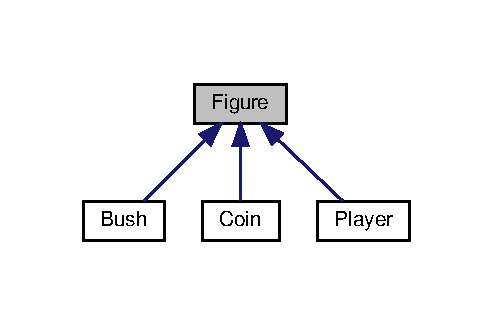
\includegraphics[width=237pt]{dc/db1/classFigure__inherit__graph}
\end{center}
\end{figure}
\subsection*{Public Member Functions}
\begin{DoxyCompactItemize}
\item 
virtual \hyperlink{classFigure_a654f8f4944edcfb248fb86b77b8b21d3}{$\sim$\+Figure} ()
\item 
virtual void \hyperlink{classFigure_ac16583e764bdc244076957bf775e4866}{draw} (\hyperlink{structvec2}{vec2} position) const =0
\end{DoxyCompactItemize}


\subsection{Constructor \& Destructor Documentation}
\mbox{\Hypertarget{classFigure_a654f8f4944edcfb248fb86b77b8b21d3}\label{classFigure_a654f8f4944edcfb248fb86b77b8b21d3}} 
\index{Figure@{Figure}!````~Figure@{$\sim$\+Figure}}
\index{````~Figure@{$\sim$\+Figure}!Figure@{Figure}}
\subsubsection{\texorpdfstring{$\sim$\+Figure()}{~Figure()}}
{\footnotesize\ttfamily virtual Figure\+::$\sim$\+Figure (\begin{DoxyParamCaption}{ }\end{DoxyParamCaption})\hspace{0.3cm}{\ttfamily [inline]}, {\ttfamily [virtual]}}



\subsection{Member Function Documentation}
\mbox{\Hypertarget{classFigure_ac16583e764bdc244076957bf775e4866}\label{classFigure_ac16583e764bdc244076957bf775e4866}} 
\index{Figure@{Figure}!draw@{draw}}
\index{draw@{draw}!Figure@{Figure}}
\subsubsection{\texorpdfstring{draw()}{draw()}}
{\footnotesize\ttfamily virtual void Figure\+::draw (\begin{DoxyParamCaption}\item[{\hyperlink{structvec2}{vec2}}]{position }\end{DoxyParamCaption}) const\hspace{0.3cm}{\ttfamily [pure virtual]}}



Implemented in \hyperlink{classPlayer_adcaf37d2753307e8a7672bd32c441576}{Player}, \hyperlink{classBush_aa73b14744dbe2b868142dc2deae485ba}{Bush}, and \hyperlink{classCoin_a13812f35d85e19553fe36350c947204c}{Coin}.



The documentation for this class was generated from the following file\+:\begin{DoxyCompactItemize}
\item 
\hyperlink{figure_8h}{figure.\+h}\end{DoxyCompactItemize}

\hypertarget{classGame}{}\section{Game Class Reference}
\label{classGame}\index{Game@{Game}}


{\ttfamily \#include $<$game.\+h$>$}



Collaboration diagram for Game\+:
\nopagebreak
\begin{figure}[H]
\begin{center}
\leavevmode
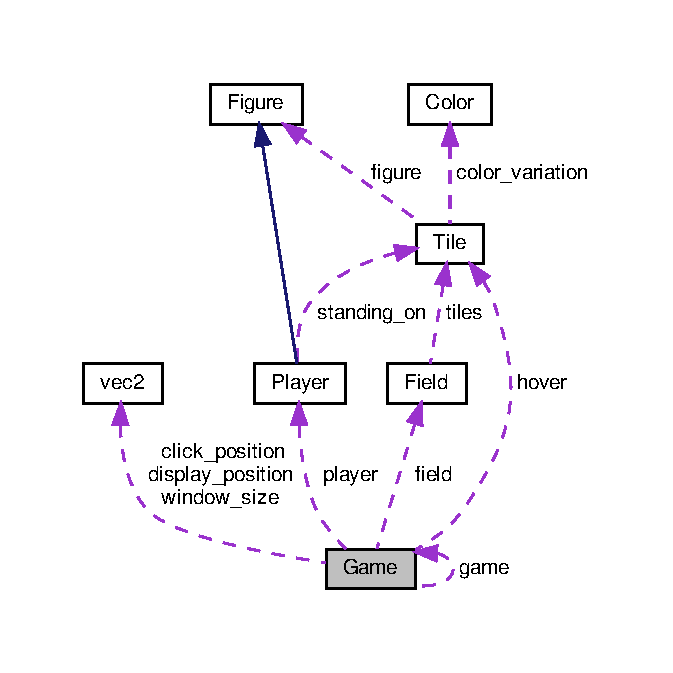
\includegraphics[width=323pt]{de/da7/classGame__coll__graph}
\end{center}
\end{figure}
\subsection*{Public Member Functions}
\begin{DoxyCompactItemize}
\item 
void \hyperlink{classGame_a6d54497ce3a66f6dd45eacfdccc8d0bd}{draw} ()
\item 
void \hyperlink{classGame_a0d2c45b51376f114fe8962d272f26c1f}{mouse} (int button, int state, int x, int y)
\item 
void \hyperlink{classGame_a6c5b84f9376ef6ce1ed2c0eeb551ff71}{keyboard} (unsigned char c, int x, int y)
\item 
void \hyperlink{classGame_af56f813ded5dbb01083c3e673fa2090b}{mousemotion} (int x, int y)
\item 
void \hyperlink{classGame_a542105a9f25169e14ca19a842d74789d}{passivmouse} (int x, int y)
\item 
void \hyperlink{classGame_ac173432416c0c8d549080c50a2fddf71}{reshape} (int width, int height)
\end{DoxyCompactItemize}
\subsection*{Static Public Member Functions}
\begin{DoxyCompactItemize}
\item 
static \hyperlink{classGame}{Game} $\ast$ \hyperlink{classGame_a19798a4f4c50037e1c5cd8c5d491fef9}{get\+Instance} ()
\item 
static void \hyperlink{classGame_a512ae0e27fd506ed300d975ed3a18f73}{init} (int $\ast$argc, char $\ast$$\ast$argv, \hyperlink{structvec2}{vec2} size)
\end{DoxyCompactItemize}
\subsection*{Private Member Functions}
\begin{DoxyCompactItemize}
\item 
\hyperlink{classGame_a9d6d7d14009e53d647a16ff1523d8639}{Game} (int $\ast$argc, char $\ast$$\ast$argv, \hyperlink{structvec2}{vec2} size)
\item 
\hyperlink{classGame_aa79443880de5f26387c2a1c70c8c1aae}{Game} (const \hyperlink{classGame}{Game} \&)
\item 
\hyperlink{classGame_ae3d112ca6e0e55150d2fdbc704474530}{$\sim$\+Game} ()
\item 
\hyperlink{classGame}{Game} \hyperlink{classGame_ad49ec11a59d863479784cac379ea47f1}{operator=} (const \hyperlink{classGame}{Game} \&)
\item 
bool \hyperlink{classGame_aae6b9f31b51dfd44e23d3d9aa18f7fe8}{move\+\_\+player\+\_\+to} (\hyperlink{classTile}{Tile} $\ast$tile)
\item 
\hyperlink{structvec2}{vec2} \hyperlink{classGame_a1946c2dd23aadfed4d91944f862294e8}{get\+Field\+Position} (int x, int y)
\item 
void \hyperlink{classGame_ad85b7db122d5d99f7a37021dbecd938a}{reload\+Matrix} ()
\end{DoxyCompactItemize}
\subsection*{Private Attributes}
\begin{DoxyCompactItemize}
\item 
\hyperlink{structvec2}{vec2} \hyperlink{classGame_abdc173d73c899329b1f3ed21b59508ee}{window\+\_\+size}
\item 
\hyperlink{structvec2}{vec2} \hyperlink{classGame_a1a2c78dbc5097d8ee63f1765c35b2410}{display\+\_\+position}
\item 
\hyperlink{structvec2}{vec2} \hyperlink{classGame_a42ff0c2859d65daadc20b3369f2233b0}{click\+\_\+position}
\item 
float \hyperlink{classGame_acf74ecf2e7981d8abe668305a77af96a}{zoom}
\item 
\hyperlink{classField}{Field} $\ast$ \hyperlink{classGame_a3cae3709d3d57b9f128e3eb98c84ba32}{field}
\item 
\hyperlink{classPlayer}{Player} $\ast$ \hyperlink{classGame_abec70aa1c0269a9a7e171af4d79e08bf}{player}
\item 
\hyperlink{classTile}{Tile} $\ast$ \hyperlink{classGame_aa71eaba68ed3622567950659638b997e}{hover}
\end{DoxyCompactItemize}
\subsection*{Static Private Attributes}
\begin{DoxyCompactItemize}
\item 
static \hyperlink{classGame}{Game} $\ast$ \hyperlink{classGame_ab652813f5a3cffb0ef4bfd08345b99ce}{game} = nullptr
\end{DoxyCompactItemize}


\subsection{Detailed Description}
\hyperlink{classGame}{Game} Class for gameing 

\subsection{Constructor \& Destructor Documentation}
\mbox{\Hypertarget{classGame_a9d6d7d14009e53d647a16ff1523d8639}\label{classGame_a9d6d7d14009e53d647a16ff1523d8639}} 
\index{Game@{Game}!Game@{Game}}
\index{Game@{Game}!Game@{Game}}
\subsubsection{\texorpdfstring{Game()}{Game()}\hspace{0.1cm}{\footnotesize\ttfamily [1/2]}}
{\footnotesize\ttfamily Game\+::\+Game (\begin{DoxyParamCaption}\item[{int $\ast$}]{argc,  }\item[{char $\ast$$\ast$}]{argv,  }\item[{\hyperlink{structvec2}{vec2}}]{size }\end{DoxyParamCaption})\hspace{0.3cm}{\ttfamily [private]}}

Constructs \hyperlink{classGame}{Game}. \mbox{\Hypertarget{classGame_aa79443880de5f26387c2a1c70c8c1aae}\label{classGame_aa79443880de5f26387c2a1c70c8c1aae}} 
\index{Game@{Game}!Game@{Game}}
\index{Game@{Game}!Game@{Game}}
\subsubsection{\texorpdfstring{Game()}{Game()}\hspace{0.1cm}{\footnotesize\ttfamily [2/2]}}
{\footnotesize\ttfamily Game\+::\+Game (\begin{DoxyParamCaption}\item[{const \hyperlink{classGame}{Game} \&}]{ }\end{DoxyParamCaption})\hspace{0.3cm}{\ttfamily [private]}}

\mbox{\Hypertarget{classGame_ae3d112ca6e0e55150d2fdbc704474530}\label{classGame_ae3d112ca6e0e55150d2fdbc704474530}} 
\index{Game@{Game}!````~Game@{$\sim$\+Game}}
\index{````~Game@{$\sim$\+Game}!Game@{Game}}
\subsubsection{\texorpdfstring{$\sim$\+Game()}{~Game()}}
{\footnotesize\ttfamily Game\+::$\sim$\+Game (\begin{DoxyParamCaption}{ }\end{DoxyParamCaption})\hspace{0.3cm}{\ttfamily [private]}}

Delets game 

\subsection{Member Function Documentation}
\mbox{\Hypertarget{classGame_a6d54497ce3a66f6dd45eacfdccc8d0bd}\label{classGame_a6d54497ce3a66f6dd45eacfdccc8d0bd}} 
\index{Game@{Game}!draw@{draw}}
\index{draw@{draw}!Game@{Game}}
\subsubsection{\texorpdfstring{draw()}{draw()}}
{\footnotesize\ttfamily void Game\+::draw (\begin{DoxyParamCaption}{ }\end{DoxyParamCaption})}

Redraw \hyperlink{classGame}{Game}. \mbox{\Hypertarget{classGame_a1946c2dd23aadfed4d91944f862294e8}\label{classGame_a1946c2dd23aadfed4d91944f862294e8}} 
\index{Game@{Game}!get\+Field\+Position@{get\+Field\+Position}}
\index{get\+Field\+Position@{get\+Field\+Position}!Game@{Game}}
\subsubsection{\texorpdfstring{get\+Field\+Position()}{getFieldPosition()}}
{\footnotesize\ttfamily \hyperlink{structvec2}{vec2} Game\+::get\+Field\+Position (\begin{DoxyParamCaption}\item[{int}]{x,  }\item[{int}]{y }\end{DoxyParamCaption})\hspace{0.3cm}{\ttfamily [private]}}

\mbox{\Hypertarget{classGame_a19798a4f4c50037e1c5cd8c5d491fef9}\label{classGame_a19798a4f4c50037e1c5cd8c5d491fef9}} 
\index{Game@{Game}!get\+Instance@{get\+Instance}}
\index{get\+Instance@{get\+Instance}!Game@{Game}}
\subsubsection{\texorpdfstring{get\+Instance()}{getInstance()}}
{\footnotesize\ttfamily \hyperlink{classGame}{Game} $\ast$ Game\+::get\+Instance (\begin{DoxyParamCaption}{ }\end{DoxyParamCaption})\hspace{0.3cm}{\ttfamily [static]}}

\begin{DoxyReturn}{Returns}
Instance of game 
\end{DoxyReturn}
\mbox{\Hypertarget{classGame_a512ae0e27fd506ed300d975ed3a18f73}\label{classGame_a512ae0e27fd506ed300d975ed3a18f73}} 
\index{Game@{Game}!init@{init}}
\index{init@{init}!Game@{Game}}
\subsubsection{\texorpdfstring{init()}{init()}}
{\footnotesize\ttfamily void Game\+::init (\begin{DoxyParamCaption}\item[{int $\ast$}]{argc,  }\item[{char $\ast$$\ast$}]{argv,  }\item[{\hyperlink{structvec2}{vec2}}]{size }\end{DoxyParamCaption})\hspace{0.3cm}{\ttfamily [static]}}

Initilice singelton Instance. \mbox{\Hypertarget{classGame_a6c5b84f9376ef6ce1ed2c0eeb551ff71}\label{classGame_a6c5b84f9376ef6ce1ed2c0eeb551ff71}} 
\index{Game@{Game}!keyboard@{keyboard}}
\index{keyboard@{keyboard}!Game@{Game}}
\subsubsection{\texorpdfstring{keyboard()}{keyboard()}}
{\footnotesize\ttfamily void Game\+::keyboard (\begin{DoxyParamCaption}\item[{unsigned char}]{c,  }\item[{int}]{x,  }\item[{int}]{y }\end{DoxyParamCaption})}

Handel Keyboard inputs. \mbox{\Hypertarget{classGame_a0d2c45b51376f114fe8962d272f26c1f}\label{classGame_a0d2c45b51376f114fe8962d272f26c1f}} 
\index{Game@{Game}!mouse@{mouse}}
\index{mouse@{mouse}!Game@{Game}}
\subsubsection{\texorpdfstring{mouse()}{mouse()}}
{\footnotesize\ttfamily void Game\+::mouse (\begin{DoxyParamCaption}\item[{int}]{button,  }\item[{int}]{state,  }\item[{int}]{x,  }\item[{int}]{y }\end{DoxyParamCaption})}

Handels Mouse Inputs \mbox{\Hypertarget{classGame_af56f813ded5dbb01083c3e673fa2090b}\label{classGame_af56f813ded5dbb01083c3e673fa2090b}} 
\index{Game@{Game}!mousemotion@{mousemotion}}
\index{mousemotion@{mousemotion}!Game@{Game}}
\subsubsection{\texorpdfstring{mousemotion()}{mousemotion()}}
{\footnotesize\ttfamily void Game\+::mousemotion (\begin{DoxyParamCaption}\item[{int}]{x,  }\item[{int}]{y }\end{DoxyParamCaption})}

\mbox{\Hypertarget{classGame_aae6b9f31b51dfd44e23d3d9aa18f7fe8}\label{classGame_aae6b9f31b51dfd44e23d3d9aa18f7fe8}} 
\index{Game@{Game}!move\+\_\+player\+\_\+to@{move\+\_\+player\+\_\+to}}
\index{move\+\_\+player\+\_\+to@{move\+\_\+player\+\_\+to}!Game@{Game}}
\subsubsection{\texorpdfstring{move\+\_\+player\+\_\+to()}{move\_player\_to()}}
{\footnotesize\ttfamily bool Game\+::move\+\_\+player\+\_\+to (\begin{DoxyParamCaption}\item[{\hyperlink{classTile}{Tile} $\ast$}]{tile }\end{DoxyParamCaption})\hspace{0.3cm}{\ttfamily [private]}}

Handels a move request. \mbox{\Hypertarget{classGame_ad49ec11a59d863479784cac379ea47f1}\label{classGame_ad49ec11a59d863479784cac379ea47f1}} 
\index{Game@{Game}!operator=@{operator=}}
\index{operator=@{operator=}!Game@{Game}}
\subsubsection{\texorpdfstring{operator=()}{operator=()}}
{\footnotesize\ttfamily \hyperlink{classGame}{Game} Game\+::operator= (\begin{DoxyParamCaption}\item[{const \hyperlink{classGame}{Game} \&}]{ }\end{DoxyParamCaption})\hspace{0.3cm}{\ttfamily [private]}}

\mbox{\Hypertarget{classGame_a542105a9f25169e14ca19a842d74789d}\label{classGame_a542105a9f25169e14ca19a842d74789d}} 
\index{Game@{Game}!passivmouse@{passivmouse}}
\index{passivmouse@{passivmouse}!Game@{Game}}
\subsubsection{\texorpdfstring{passivmouse()}{passivmouse()}}
{\footnotesize\ttfamily void Game\+::passivmouse (\begin{DoxyParamCaption}\item[{int}]{x,  }\item[{int}]{y }\end{DoxyParamCaption})}

\mbox{\Hypertarget{classGame_ad85b7db122d5d99f7a37021dbecd938a}\label{classGame_ad85b7db122d5d99f7a37021dbecd938a}} 
\index{Game@{Game}!reload\+Matrix@{reload\+Matrix}}
\index{reload\+Matrix@{reload\+Matrix}!Game@{Game}}
\subsubsection{\texorpdfstring{reload\+Matrix()}{reloadMatrix()}}
{\footnotesize\ttfamily void Game\+::reload\+Matrix (\begin{DoxyParamCaption}{ }\end{DoxyParamCaption})\hspace{0.3cm}{\ttfamily [private]}}

Resets Projectoin Matrix for Rendering. \mbox{\Hypertarget{classGame_ac173432416c0c8d549080c50a2fddf71}\label{classGame_ac173432416c0c8d549080c50a2fddf71}} 
\index{Game@{Game}!reshape@{reshape}}
\index{reshape@{reshape}!Game@{Game}}
\subsubsection{\texorpdfstring{reshape()}{reshape()}}
{\footnotesize\ttfamily void Game\+::reshape (\begin{DoxyParamCaption}\item[{int}]{width,  }\item[{int}]{height }\end{DoxyParamCaption})}



\subsection{Member Data Documentation}
\mbox{\Hypertarget{classGame_a42ff0c2859d65daadc20b3369f2233b0}\label{classGame_a42ff0c2859d65daadc20b3369f2233b0}} 
\index{Game@{Game}!click\+\_\+position@{click\+\_\+position}}
\index{click\+\_\+position@{click\+\_\+position}!Game@{Game}}
\subsubsection{\texorpdfstring{click\+\_\+position}{click\_position}}
{\footnotesize\ttfamily \hyperlink{structvec2}{vec2} Game\+::click\+\_\+position\hspace{0.3cm}{\ttfamily [private]}}

\mbox{\Hypertarget{classGame_a1a2c78dbc5097d8ee63f1765c35b2410}\label{classGame_a1a2c78dbc5097d8ee63f1765c35b2410}} 
\index{Game@{Game}!display\+\_\+position@{display\+\_\+position}}
\index{display\+\_\+position@{display\+\_\+position}!Game@{Game}}
\subsubsection{\texorpdfstring{display\+\_\+position}{display\_position}}
{\footnotesize\ttfamily \hyperlink{structvec2}{vec2} Game\+::display\+\_\+position\hspace{0.3cm}{\ttfamily [private]}}

\mbox{\Hypertarget{classGame_a3cae3709d3d57b9f128e3eb98c84ba32}\label{classGame_a3cae3709d3d57b9f128e3eb98c84ba32}} 
\index{Game@{Game}!field@{field}}
\index{field@{field}!Game@{Game}}
\subsubsection{\texorpdfstring{field}{field}}
{\footnotesize\ttfamily \hyperlink{classField}{Field}$\ast$ Game\+::field\hspace{0.3cm}{\ttfamily [private]}}

\mbox{\Hypertarget{classGame_ab652813f5a3cffb0ef4bfd08345b99ce}\label{classGame_ab652813f5a3cffb0ef4bfd08345b99ce}} 
\index{Game@{Game}!game@{game}}
\index{game@{game}!Game@{Game}}
\subsubsection{\texorpdfstring{game}{game}}
{\footnotesize\ttfamily \hyperlink{classGame}{Game} $\ast$ Game\+::game = nullptr\hspace{0.3cm}{\ttfamily [static]}, {\ttfamily [private]}}

Singelton Instance. \mbox{\Hypertarget{classGame_aa71eaba68ed3622567950659638b997e}\label{classGame_aa71eaba68ed3622567950659638b997e}} 
\index{Game@{Game}!hover@{hover}}
\index{hover@{hover}!Game@{Game}}
\subsubsection{\texorpdfstring{hover}{hover}}
{\footnotesize\ttfamily \hyperlink{classTile}{Tile}$\ast$ Game\+::hover\hspace{0.3cm}{\ttfamily [private]}}

\mbox{\Hypertarget{classGame_abec70aa1c0269a9a7e171af4d79e08bf}\label{classGame_abec70aa1c0269a9a7e171af4d79e08bf}} 
\index{Game@{Game}!player@{player}}
\index{player@{player}!Game@{Game}}
\subsubsection{\texorpdfstring{player}{player}}
{\footnotesize\ttfamily \hyperlink{classPlayer}{Player}$\ast$ Game\+::player\hspace{0.3cm}{\ttfamily [private]}}

\mbox{\Hypertarget{classGame_abdc173d73c899329b1f3ed21b59508ee}\label{classGame_abdc173d73c899329b1f3ed21b59508ee}} 
\index{Game@{Game}!window\+\_\+size@{window\+\_\+size}}
\index{window\+\_\+size@{window\+\_\+size}!Game@{Game}}
\subsubsection{\texorpdfstring{window\+\_\+size}{window\_size}}
{\footnotesize\ttfamily \hyperlink{structvec2}{vec2} Game\+::window\+\_\+size\hspace{0.3cm}{\ttfamily [private]}}

\mbox{\Hypertarget{classGame_acf74ecf2e7981d8abe668305a77af96a}\label{classGame_acf74ecf2e7981d8abe668305a77af96a}} 
\index{Game@{Game}!zoom@{zoom}}
\index{zoom@{zoom}!Game@{Game}}
\subsubsection{\texorpdfstring{zoom}{zoom}}
{\footnotesize\ttfamily float Game\+::zoom\hspace{0.3cm}{\ttfamily [private]}}



The documentation for this class was generated from the following files\+:\begin{DoxyCompactItemize}
\item 
\hyperlink{game_8h}{game.\+h}\item 
\hyperlink{game_8cpp}{game.\+cpp}\end{DoxyCompactItemize}

\hypertarget{classPlayer}{}\section{Player Class Reference}
\label{classPlayer}\index{Player@{Player}}


{\ttfamily \#include $<$player.\+h$>$}



Inheritance diagram for Player\+:
\nopagebreak
\begin{figure}[H]
\begin{center}
\leavevmode
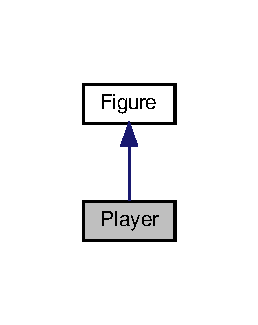
\includegraphics[width=124pt]{df/da4/classPlayer__inherit__graph}
\end{center}
\end{figure}


Collaboration diagram for Player\+:
\nopagebreak
\begin{figure}[H]
\begin{center}
\leavevmode
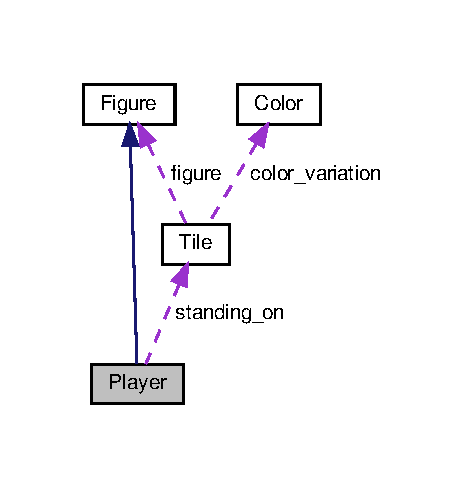
\includegraphics[width=224pt]{dc/d25/classPlayer__coll__graph}
\end{center}
\end{figure}
\subsection*{Public Member Functions}
\begin{DoxyCompactItemize}
\item 
\hyperlink{classPlayer_a5a23c2fa4df597d3b41e068f0c54ea8a}{Player} (\hyperlink{classTile}{Tile} $\ast$\+\_\+standing\+\_\+on)
\item 
void \hyperlink{classPlayer_ae330dc5684cee833dede7f3728d60a90}{move} (\hyperlink{classTile}{Tile} $\ast$move\+\_\+to)
\item 
void \hyperlink{classPlayer_adcaf37d2753307e8a7672bd32c441576}{draw} (\hyperlink{structvec2}{vec2} position) const
\end{DoxyCompactItemize}
\subsection*{Public Attributes}
\begin{DoxyCompactItemize}
\item 
\hyperlink{classTile}{Tile} $\ast$ \hyperlink{classPlayer_a7193ba7104612cf2ddecee5fbbe6f063}{standing\+\_\+on} = nullptr
\end{DoxyCompactItemize}


\subsection{Constructor \& Destructor Documentation}
\mbox{\Hypertarget{classPlayer_a5a23c2fa4df597d3b41e068f0c54ea8a}\label{classPlayer_a5a23c2fa4df597d3b41e068f0c54ea8a}} 
\index{Player@{Player}!Player@{Player}}
\index{Player@{Player}!Player@{Player}}
\subsubsection{\texorpdfstring{Player()}{Player()}}
{\footnotesize\ttfamily Player\+::\+Player (\begin{DoxyParamCaption}\item[{\hyperlink{classTile}{Tile} $\ast$}]{\+\_\+standing\+\_\+on }\end{DoxyParamCaption})\hspace{0.3cm}{\ttfamily [inline]}}



\subsection{Member Function Documentation}
\mbox{\Hypertarget{classPlayer_adcaf37d2753307e8a7672bd32c441576}\label{classPlayer_adcaf37d2753307e8a7672bd32c441576}} 
\index{Player@{Player}!draw@{draw}}
\index{draw@{draw}!Player@{Player}}
\subsubsection{\texorpdfstring{draw()}{draw()}}
{\footnotesize\ttfamily void Player\+::draw (\begin{DoxyParamCaption}\item[{\hyperlink{structvec2}{vec2}}]{position }\end{DoxyParamCaption}) const\hspace{0.3cm}{\ttfamily [virtual]}}



Implements \hyperlink{classFigure_ac16583e764bdc244076957bf775e4866}{Figure}.

\mbox{\Hypertarget{classPlayer_ae330dc5684cee833dede7f3728d60a90}\label{classPlayer_ae330dc5684cee833dede7f3728d60a90}} 
\index{Player@{Player}!move@{move}}
\index{move@{move}!Player@{Player}}
\subsubsection{\texorpdfstring{move()}{move()}}
{\footnotesize\ttfamily void Player\+::move (\begin{DoxyParamCaption}\item[{\hyperlink{classTile}{Tile} $\ast$}]{move\+\_\+to }\end{DoxyParamCaption})\hspace{0.3cm}{\ttfamily [inline]}}



\subsection{Member Data Documentation}
\mbox{\Hypertarget{classPlayer_a7193ba7104612cf2ddecee5fbbe6f063}\label{classPlayer_a7193ba7104612cf2ddecee5fbbe6f063}} 
\index{Player@{Player}!standing\+\_\+on@{standing\+\_\+on}}
\index{standing\+\_\+on@{standing\+\_\+on}!Player@{Player}}
\subsubsection{\texorpdfstring{standing\+\_\+on}{standing\_on}}
{\footnotesize\ttfamily \hyperlink{classTile}{Tile}$\ast$ Player\+::standing\+\_\+on = nullptr}



The documentation for this class was generated from the following files\+:\begin{DoxyCompactItemize}
\item 
\hyperlink{player_8h}{player.\+h}\item 
\hyperlink{player_8cpp}{player.\+cpp}\end{DoxyCompactItemize}

\hypertarget{classTile}{}\section{Tile Class Reference}
\label{classTile}\index{Tile@{Tile}}


{\ttfamily \#include $<$tile.\+h$>$}



Collaboration diagram for Tile\+:
\nopagebreak
\begin{figure}[H]
\begin{center}
\leavevmode
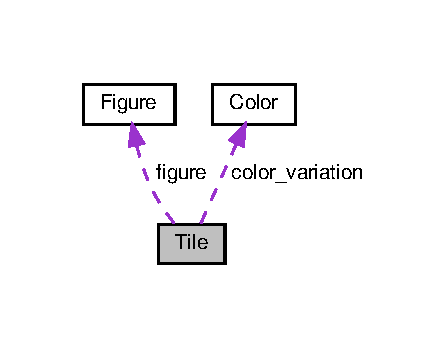
\includegraphics[width=215pt]{d6/dd1/classTile__coll__graph}
\end{center}
\end{figure}
\subsection*{Public Member Functions}
\begin{DoxyCompactItemize}
\item 
\hyperlink{classTile_aeeb5593bb6b75aae2edfcccbc84ab378}{Tile} ()
\item 
\hyperlink{classTile_a98634abbd93fa13d0578d7103202d03d}{$\sim$\+Tile} ()
\item 
\hyperlink{classFigure}{Figure} $\ast$\& \hyperlink{classTile_a60af31824ef9a5992f9e17b13df76c60}{get\+Figure} ()
\item 
bool \hyperlink{classTile_a1cb171d83f6942aebd2499bc2c678f7f}{place} (\hyperlink{classFigure}{Figure} $\ast$fig)
\item 
void \hyperlink{classTile_a8f482bab4aa537311f8948f225c915a4}{clear} ()
\item 
void \hyperlink{classTile_a2df9b57eb3fdba56aa69d989c18a7989}{raise} (int amount)
\item 
void \hyperlink{classTile_a69a295280f0ab2c2e5325ed3aabaf54e}{move\+Figure\+To} (\hyperlink{classTile}{Tile} $\ast$tile)
\item 
int \hyperlink{classTile_a8ff17f88b15ff106a8df470df9b4bda6}{get\+Height} () const
\item 
bool \hyperlink{classTile_a2f9971efdf7b36249a491ca7ceb2ef57}{is\+Walkable} () const
\item 
void \hyperlink{classTile_ab0e0884c673e59a98e59118fa92127bc}{draw} (\hyperlink{structvec2}{vec2} position, const std\+::map$<$ int, \hyperlink{structColor}{Color} $>$ \&color\+\_\+map) const
\item 
void \hyperlink{classTile_afe81f76a0c23b9050990e0f10eb4128f}{mark} (\hyperlink{structvec2}{vec2} translation) const
\item 
void \hyperlink{classTile_a872043e678348699184b5d55efb4c6d3}{plant} ()
\end{DoxyCompactItemize}
\subsection*{Private Member Functions}
\begin{DoxyCompactItemize}
\item 
\hyperlink{classTile_a0118b16957fc9fc912905c3085afe926}{Tile} (const \hyperlink{classTile}{Tile} \&tile)=delete
\item 
const \hyperlink{classTile}{Tile} \& \hyperlink{classTile_a75da44d88e876130202f7dfddec72121}{operator=} (const \hyperlink{classTile}{Tile} \&tile)=delete
\end{DoxyCompactItemize}
\subsection*{Private Attributes}
\begin{DoxyCompactItemize}
\item 
\hyperlink{classFigure}{Figure} $\ast$ \hyperlink{classTile_a96976c70d77812bcce266c00ba0513ee}{figure}
\item 
\hyperlink{structColor}{Color} \hyperlink{classTile_abfdce38f0f708b67dd84e0992ebca268}{color\+\_\+variation}
\item 
int \hyperlink{classTile_a1ceee2a6a986af91980d62c039ffe792}{height}
\end{DoxyCompactItemize}


\subsection{Constructor \& Destructor Documentation}
\mbox{\Hypertarget{classTile_a0118b16957fc9fc912905c3085afe926}\label{classTile_a0118b16957fc9fc912905c3085afe926}} 
\index{Tile@{Tile}!Tile@{Tile}}
\index{Tile@{Tile}!Tile@{Tile}}
\subsubsection{\texorpdfstring{Tile()}{Tile()}\hspace{0.1cm}{\footnotesize\ttfamily [1/2]}}
{\footnotesize\ttfamily Tile\+::\+Tile (\begin{DoxyParamCaption}\item[{const \hyperlink{classTile}{Tile} \&}]{tile }\end{DoxyParamCaption})\hspace{0.3cm}{\ttfamily [private]}, {\ttfamily [delete]}}

\mbox{\Hypertarget{classTile_aeeb5593bb6b75aae2edfcccbc84ab378}\label{classTile_aeeb5593bb6b75aae2edfcccbc84ab378}} 
\index{Tile@{Tile}!Tile@{Tile}}
\index{Tile@{Tile}!Tile@{Tile}}
\subsubsection{\texorpdfstring{Tile()}{Tile()}\hspace{0.1cm}{\footnotesize\ttfamily [2/2]}}
{\footnotesize\ttfamily Tile\+::\+Tile (\begin{DoxyParamCaption}{ }\end{DoxyParamCaption})\hspace{0.3cm}{\ttfamily [inline]}}

\mbox{\Hypertarget{classTile_a98634abbd93fa13d0578d7103202d03d}\label{classTile_a98634abbd93fa13d0578d7103202d03d}} 
\index{Tile@{Tile}!````~Tile@{$\sim$\+Tile}}
\index{````~Tile@{$\sim$\+Tile}!Tile@{Tile}}
\subsubsection{\texorpdfstring{$\sim$\+Tile()}{~Tile()}}
{\footnotesize\ttfamily Tile\+::$\sim$\+Tile (\begin{DoxyParamCaption}{ }\end{DoxyParamCaption})\hspace{0.3cm}{\ttfamily [inline]}}



\subsection{Member Function Documentation}
\mbox{\Hypertarget{classTile_a8f482bab4aa537311f8948f225c915a4}\label{classTile_a8f482bab4aa537311f8948f225c915a4}} 
\index{Tile@{Tile}!clear@{clear}}
\index{clear@{clear}!Tile@{Tile}}
\subsubsection{\texorpdfstring{clear()}{clear()}}
{\footnotesize\ttfamily void Tile\+::clear (\begin{DoxyParamCaption}{ }\end{DoxyParamCaption})\hspace{0.3cm}{\ttfamily [inline]}}

\mbox{\Hypertarget{classTile_ab0e0884c673e59a98e59118fa92127bc}\label{classTile_ab0e0884c673e59a98e59118fa92127bc}} 
\index{Tile@{Tile}!draw@{draw}}
\index{draw@{draw}!Tile@{Tile}}
\subsubsection{\texorpdfstring{draw()}{draw()}}
{\footnotesize\ttfamily void Tile\+::draw (\begin{DoxyParamCaption}\item[{\hyperlink{structvec2}{vec2}}]{position,  }\item[{const std\+::map$<$ int, \hyperlink{structColor}{Color} $>$ \&}]{color\+\_\+map }\end{DoxyParamCaption}) const}

\mbox{\Hypertarget{classTile_a60af31824ef9a5992f9e17b13df76c60}\label{classTile_a60af31824ef9a5992f9e17b13df76c60}} 
\index{Tile@{Tile}!get\+Figure@{get\+Figure}}
\index{get\+Figure@{get\+Figure}!Tile@{Tile}}
\subsubsection{\texorpdfstring{get\+Figure()}{getFigure()}}
{\footnotesize\ttfamily \hyperlink{classFigure}{Figure}$\ast$\& Tile\+::get\+Figure (\begin{DoxyParamCaption}{ }\end{DoxyParamCaption})\hspace{0.3cm}{\ttfamily [inline]}}

\mbox{\Hypertarget{classTile_a8ff17f88b15ff106a8df470df9b4bda6}\label{classTile_a8ff17f88b15ff106a8df470df9b4bda6}} 
\index{Tile@{Tile}!get\+Height@{get\+Height}}
\index{get\+Height@{get\+Height}!Tile@{Tile}}
\subsubsection{\texorpdfstring{get\+Height()}{getHeight()}}
{\footnotesize\ttfamily int Tile\+::get\+Height (\begin{DoxyParamCaption}{ }\end{DoxyParamCaption}) const\hspace{0.3cm}{\ttfamily [inline]}}

\mbox{\Hypertarget{classTile_a2f9971efdf7b36249a491ca7ceb2ef57}\label{classTile_a2f9971efdf7b36249a491ca7ceb2ef57}} 
\index{Tile@{Tile}!is\+Walkable@{is\+Walkable}}
\index{is\+Walkable@{is\+Walkable}!Tile@{Tile}}
\subsubsection{\texorpdfstring{is\+Walkable()}{isWalkable()}}
{\footnotesize\ttfamily bool Tile\+::is\+Walkable (\begin{DoxyParamCaption}{ }\end{DoxyParamCaption}) const\hspace{0.3cm}{\ttfamily [inline]}}

\mbox{\Hypertarget{classTile_afe81f76a0c23b9050990e0f10eb4128f}\label{classTile_afe81f76a0c23b9050990e0f10eb4128f}} 
\index{Tile@{Tile}!mark@{mark}}
\index{mark@{mark}!Tile@{Tile}}
\subsubsection{\texorpdfstring{mark()}{mark()}}
{\footnotesize\ttfamily void Tile\+::mark (\begin{DoxyParamCaption}\item[{\hyperlink{structvec2}{vec2}}]{translation }\end{DoxyParamCaption}) const}

\mbox{\Hypertarget{classTile_a69a295280f0ab2c2e5325ed3aabaf54e}\label{classTile_a69a295280f0ab2c2e5325ed3aabaf54e}} 
\index{Tile@{Tile}!move\+Figure\+To@{move\+Figure\+To}}
\index{move\+Figure\+To@{move\+Figure\+To}!Tile@{Tile}}
\subsubsection{\texorpdfstring{move\+Figure\+To()}{moveFigureTo()}}
{\footnotesize\ttfamily void Tile\+::move\+Figure\+To (\begin{DoxyParamCaption}\item[{\hyperlink{classTile}{Tile} $\ast$}]{tile }\end{DoxyParamCaption})\hspace{0.3cm}{\ttfamily [inline]}}

\mbox{\Hypertarget{classTile_a75da44d88e876130202f7dfddec72121}\label{classTile_a75da44d88e876130202f7dfddec72121}} 
\index{Tile@{Tile}!operator=@{operator=}}
\index{operator=@{operator=}!Tile@{Tile}}
\subsubsection{\texorpdfstring{operator=()}{operator=()}}
{\footnotesize\ttfamily const \hyperlink{classTile}{Tile}\& Tile\+::operator= (\begin{DoxyParamCaption}\item[{const \hyperlink{classTile}{Tile} \&}]{tile }\end{DoxyParamCaption})\hspace{0.3cm}{\ttfamily [private]}, {\ttfamily [delete]}}

\mbox{\Hypertarget{classTile_a1cb171d83f6942aebd2499bc2c678f7f}\label{classTile_a1cb171d83f6942aebd2499bc2c678f7f}} 
\index{Tile@{Tile}!place@{place}}
\index{place@{place}!Tile@{Tile}}
\subsubsection{\texorpdfstring{place()}{place()}}
{\footnotesize\ttfamily bool Tile\+::place (\begin{DoxyParamCaption}\item[{\hyperlink{classFigure}{Figure} $\ast$}]{fig }\end{DoxyParamCaption})\hspace{0.3cm}{\ttfamily [inline]}}

\mbox{\Hypertarget{classTile_a872043e678348699184b5d55efb4c6d3}\label{classTile_a872043e678348699184b5d55efb4c6d3}} 
\index{Tile@{Tile}!plant@{plant}}
\index{plant@{plant}!Tile@{Tile}}
\subsubsection{\texorpdfstring{plant()}{plant()}}
{\footnotesize\ttfamily void Tile\+::plant (\begin{DoxyParamCaption}{ }\end{DoxyParamCaption})\hspace{0.3cm}{\ttfamily [inline]}}

\mbox{\Hypertarget{classTile_a2df9b57eb3fdba56aa69d989c18a7989}\label{classTile_a2df9b57eb3fdba56aa69d989c18a7989}} 
\index{Tile@{Tile}!raise@{raise}}
\index{raise@{raise}!Tile@{Tile}}
\subsubsection{\texorpdfstring{raise()}{raise()}}
{\footnotesize\ttfamily void Tile\+::raise (\begin{DoxyParamCaption}\item[{int}]{amount }\end{DoxyParamCaption})\hspace{0.3cm}{\ttfamily [inline]}}



\subsection{Member Data Documentation}
\mbox{\Hypertarget{classTile_abfdce38f0f708b67dd84e0992ebca268}\label{classTile_abfdce38f0f708b67dd84e0992ebca268}} 
\index{Tile@{Tile}!color\+\_\+variation@{color\+\_\+variation}}
\index{color\+\_\+variation@{color\+\_\+variation}!Tile@{Tile}}
\subsubsection{\texorpdfstring{color\+\_\+variation}{color\_variation}}
{\footnotesize\ttfamily \hyperlink{structColor}{Color} Tile\+::color\+\_\+variation\hspace{0.3cm}{\ttfamily [private]}}

\mbox{\Hypertarget{classTile_a96976c70d77812bcce266c00ba0513ee}\label{classTile_a96976c70d77812bcce266c00ba0513ee}} 
\index{Tile@{Tile}!figure@{figure}}
\index{figure@{figure}!Tile@{Tile}}
\subsubsection{\texorpdfstring{figure}{figure}}
{\footnotesize\ttfamily \hyperlink{classFigure}{Figure}$\ast$ Tile\+::figure\hspace{0.3cm}{\ttfamily [private]}}

\mbox{\Hypertarget{classTile_a1ceee2a6a986af91980d62c039ffe792}\label{classTile_a1ceee2a6a986af91980d62c039ffe792}} 
\index{Tile@{Tile}!height@{height}}
\index{height@{height}!Tile@{Tile}}
\subsubsection{\texorpdfstring{height}{height}}
{\footnotesize\ttfamily int Tile\+::height\hspace{0.3cm}{\ttfamily [private]}}



The documentation for this class was generated from the following files\+:\begin{DoxyCompactItemize}
\item 
\hyperlink{tile_8h}{tile.\+h}\item 
\hyperlink{tile_8cpp}{tile.\+cpp}\end{DoxyCompactItemize}

\hypertarget{structvec2}{}\section{vec2 Struct Reference}
\label{structvec2}\index{vec2@{vec2}}


{\ttfamily \#include $<$vec2.\+h$>$}

\subsection*{Public Member Functions}
\begin{DoxyCompactItemize}
\item 
\hyperlink{structvec2_ae12a1a221eca3561809600a11b58eaa3}{vec2} ()
\item 
\hyperlink{structvec2_a6a3b46530cd2ed011bb5cdbbec62be26}{vec2} (float \+\_\+x, float \+\_\+y)
\item 
\hyperlink{structvec2_a0fcc1b7272d1ebd806cca02d29563053}{vec2} (const \hyperlink{structvec2}{vec2} \&other)
\item 
\hyperlink{structvec2}{vec2} \hyperlink{structvec2_a3cb4130bbf48a0234bbd70a6e5603bb2}{operator=} (const \hyperlink{structvec2}{vec2} \&rhs)
\item 
\hyperlink{structvec2_a1ae1b7c30215e766b3e56bf79112ffc1}{$\sim$vec2} ()
\item 
\hyperlink{structvec2}{vec2} \hyperlink{structvec2_a8ddc4154c0d2688aecf156a3d3ebc7c7}{operator+} (const \hyperlink{structvec2}{vec2} \&rhs) const
\item 
\hyperlink{structvec2}{vec2} \hyperlink{structvec2_ad0cc0e5f6a564ec00824bd35fe112c46}{operator+=} (const \hyperlink{structvec2}{vec2} \&rhs)
\item 
\hyperlink{structvec2}{vec2} \hyperlink{structvec2_a8951488e5d92bbd54212bacc0753c079}{operator-\/} (const \hyperlink{structvec2}{vec2} \&rhs) const
\item 
\hyperlink{structvec2}{vec2} \hyperlink{structvec2_af53cb37ea6fd794dbdaf1a1de9a5cf5c}{operator-\/=} (const \hyperlink{structvec2}{vec2} \&rhs)
\item 
\hyperlink{structvec2}{vec2} \hyperlink{structvec2_a68f9765fd1eac99396be0958e15a908c}{operator$\ast$} (float rhs) const
\item 
\hyperlink{structvec2}{vec2} \hyperlink{structvec2_aaeef9a4b188905735d1c7996dafb77cb}{operator$\ast$=} (float rhs)
\item 
\hyperlink{structvec2_a04106d6297826f99ad1eb28f2b4eb564}{operator float} () const
\item 
float \hyperlink{structvec2_a4bd69636a40be9fe1949d1a3e4b1ff50}{length\+Squared} () const
\item 
\hyperlink{structvec2}{vec2} \hyperlink{structvec2_acfc20e9984f37b033b8ace687823700c}{normalize} ()
\item 
\hyperlink{structvec2}{vec2} \hyperlink{structvec2_acb4a4c9ee8c1d81e6e51b1251e0c1f69}{normalized} () const
\end{DoxyCompactItemize}
\subsection*{Static Public Member Functions}
\begin{DoxyCompactItemize}
\item 
static float \hyperlink{structvec2_a7bb0dddaf76881c9e2cbc05c5fd6bc4b}{dot} (const \hyperlink{structvec2}{vec2} \&lhs, const \hyperlink{structvec2}{vec2} \&rhs)
\end{DoxyCompactItemize}
\subsection*{Public Attributes}
\begin{DoxyCompactItemize}
\item 
float \hyperlink{structvec2_a002d3519d48fe3cd79729b5b0ded74bf}{x}
\item 
float \hyperlink{structvec2_a6d28b12b511da692550fc9d37b4e9b1d}{y}
\end{DoxyCompactItemize}
\subsection*{Friends}
\begin{DoxyCompactItemize}
\item 
std\+::ostream \& \hyperlink{structvec2_a85b47f3582472fa5e3f80e6efd59f1d6}{operator$<$$<$} (std\+::ostream \&os, const \hyperlink{structvec2}{vec2} \&vec)
\end{DoxyCompactItemize}


\subsection{Constructor \& Destructor Documentation}
\mbox{\Hypertarget{structvec2_ae12a1a221eca3561809600a11b58eaa3}\label{structvec2_ae12a1a221eca3561809600a11b58eaa3}} 
\index{vec2@{vec2}!vec2@{vec2}}
\index{vec2@{vec2}!vec2@{vec2}}
\subsubsection{\texorpdfstring{vec2()}{vec2()}\hspace{0.1cm}{\footnotesize\ttfamily [1/3]}}
{\footnotesize\ttfamily vec2\+::vec2 (\begin{DoxyParamCaption}{ }\end{DoxyParamCaption})}

\mbox{\Hypertarget{structvec2_a6a3b46530cd2ed011bb5cdbbec62be26}\label{structvec2_a6a3b46530cd2ed011bb5cdbbec62be26}} 
\index{vec2@{vec2}!vec2@{vec2}}
\index{vec2@{vec2}!vec2@{vec2}}
\subsubsection{\texorpdfstring{vec2()}{vec2()}\hspace{0.1cm}{\footnotesize\ttfamily [2/3]}}
{\footnotesize\ttfamily vec2\+::vec2 (\begin{DoxyParamCaption}\item[{float}]{\+\_\+x,  }\item[{float}]{\+\_\+y }\end{DoxyParamCaption})}

\mbox{\Hypertarget{structvec2_a0fcc1b7272d1ebd806cca02d29563053}\label{structvec2_a0fcc1b7272d1ebd806cca02d29563053}} 
\index{vec2@{vec2}!vec2@{vec2}}
\index{vec2@{vec2}!vec2@{vec2}}
\subsubsection{\texorpdfstring{vec2()}{vec2()}\hspace{0.1cm}{\footnotesize\ttfamily [3/3]}}
{\footnotesize\ttfamily vec2\+::vec2 (\begin{DoxyParamCaption}\item[{const \hyperlink{structvec2}{vec2} \&}]{other }\end{DoxyParamCaption})}

\mbox{\Hypertarget{structvec2_a1ae1b7c30215e766b3e56bf79112ffc1}\label{structvec2_a1ae1b7c30215e766b3e56bf79112ffc1}} 
\index{vec2@{vec2}!````~vec2@{$\sim$vec2}}
\index{````~vec2@{$\sim$vec2}!vec2@{vec2}}
\subsubsection{\texorpdfstring{$\sim$vec2()}{~vec2()}}
{\footnotesize\ttfamily vec2\+::$\sim$vec2 (\begin{DoxyParamCaption}{ }\end{DoxyParamCaption})}



\subsection{Member Function Documentation}
\mbox{\Hypertarget{structvec2_a7bb0dddaf76881c9e2cbc05c5fd6bc4b}\label{structvec2_a7bb0dddaf76881c9e2cbc05c5fd6bc4b}} 
\index{vec2@{vec2}!dot@{dot}}
\index{dot@{dot}!vec2@{vec2}}
\subsubsection{\texorpdfstring{dot()}{dot()}}
{\footnotesize\ttfamily float vec2\+::dot (\begin{DoxyParamCaption}\item[{const \hyperlink{structvec2}{vec2} \&}]{lhs,  }\item[{const \hyperlink{structvec2}{vec2} \&}]{rhs }\end{DoxyParamCaption})\hspace{0.3cm}{\ttfamily [static]}}

\mbox{\Hypertarget{structvec2_a4bd69636a40be9fe1949d1a3e4b1ff50}\label{structvec2_a4bd69636a40be9fe1949d1a3e4b1ff50}} 
\index{vec2@{vec2}!length\+Squared@{length\+Squared}}
\index{length\+Squared@{length\+Squared}!vec2@{vec2}}
\subsubsection{\texorpdfstring{length\+Squared()}{lengthSquared()}}
{\footnotesize\ttfamily float vec2\+::length\+Squared (\begin{DoxyParamCaption}{ }\end{DoxyParamCaption}) const}

\mbox{\Hypertarget{structvec2_acfc20e9984f37b033b8ace687823700c}\label{structvec2_acfc20e9984f37b033b8ace687823700c}} 
\index{vec2@{vec2}!normalize@{normalize}}
\index{normalize@{normalize}!vec2@{vec2}}
\subsubsection{\texorpdfstring{normalize()}{normalize()}}
{\footnotesize\ttfamily \hyperlink{structvec2}{vec2} vec2\+::normalize (\begin{DoxyParamCaption}{ }\end{DoxyParamCaption})}

\mbox{\Hypertarget{structvec2_acb4a4c9ee8c1d81e6e51b1251e0c1f69}\label{structvec2_acb4a4c9ee8c1d81e6e51b1251e0c1f69}} 
\index{vec2@{vec2}!normalized@{normalized}}
\index{normalized@{normalized}!vec2@{vec2}}
\subsubsection{\texorpdfstring{normalized()}{normalized()}}
{\footnotesize\ttfamily \hyperlink{structvec2}{vec2} vec2\+::normalized (\begin{DoxyParamCaption}{ }\end{DoxyParamCaption}) const}

\mbox{\Hypertarget{structvec2_a04106d6297826f99ad1eb28f2b4eb564}\label{structvec2_a04106d6297826f99ad1eb28f2b4eb564}} 
\index{vec2@{vec2}!operator float@{operator float}}
\index{operator float@{operator float}!vec2@{vec2}}
\subsubsection{\texorpdfstring{operator float()}{operator float()}}
{\footnotesize\ttfamily vec2\+::operator float (\begin{DoxyParamCaption}{ }\end{DoxyParamCaption}) const}

\mbox{\Hypertarget{structvec2_a68f9765fd1eac99396be0958e15a908c}\label{structvec2_a68f9765fd1eac99396be0958e15a908c}} 
\index{vec2@{vec2}!operator$\ast$@{operator$\ast$}}
\index{operator$\ast$@{operator$\ast$}!vec2@{vec2}}
\subsubsection{\texorpdfstring{operator$\ast$()}{operator*()}}
{\footnotesize\ttfamily \hyperlink{structvec2}{vec2} vec2\+::operator$\ast$ (\begin{DoxyParamCaption}\item[{float}]{rhs }\end{DoxyParamCaption}) const}

\mbox{\Hypertarget{structvec2_aaeef9a4b188905735d1c7996dafb77cb}\label{structvec2_aaeef9a4b188905735d1c7996dafb77cb}} 
\index{vec2@{vec2}!operator$\ast$=@{operator$\ast$=}}
\index{operator$\ast$=@{operator$\ast$=}!vec2@{vec2}}
\subsubsection{\texorpdfstring{operator$\ast$=()}{operator*=()}}
{\footnotesize\ttfamily \hyperlink{structvec2}{vec2} vec2\+::operator$\ast$= (\begin{DoxyParamCaption}\item[{float}]{rhs }\end{DoxyParamCaption})}

\mbox{\Hypertarget{structvec2_a8ddc4154c0d2688aecf156a3d3ebc7c7}\label{structvec2_a8ddc4154c0d2688aecf156a3d3ebc7c7}} 
\index{vec2@{vec2}!operator+@{operator+}}
\index{operator+@{operator+}!vec2@{vec2}}
\subsubsection{\texorpdfstring{operator+()}{operator+()}}
{\footnotesize\ttfamily \hyperlink{structvec2}{vec2} vec2\+::operator+ (\begin{DoxyParamCaption}\item[{const \hyperlink{structvec2}{vec2} \&}]{rhs }\end{DoxyParamCaption}) const}

\mbox{\Hypertarget{structvec2_ad0cc0e5f6a564ec00824bd35fe112c46}\label{structvec2_ad0cc0e5f6a564ec00824bd35fe112c46}} 
\index{vec2@{vec2}!operator+=@{operator+=}}
\index{operator+=@{operator+=}!vec2@{vec2}}
\subsubsection{\texorpdfstring{operator+=()}{operator+=()}}
{\footnotesize\ttfamily \hyperlink{structvec2}{vec2} vec2\+::operator+= (\begin{DoxyParamCaption}\item[{const \hyperlink{structvec2}{vec2} \&}]{rhs }\end{DoxyParamCaption})}

\mbox{\Hypertarget{structvec2_a8951488e5d92bbd54212bacc0753c079}\label{structvec2_a8951488e5d92bbd54212bacc0753c079}} 
\index{vec2@{vec2}!operator-\/@{operator-\/}}
\index{operator-\/@{operator-\/}!vec2@{vec2}}
\subsubsection{\texorpdfstring{operator-\/()}{operator-()}}
{\footnotesize\ttfamily \hyperlink{structvec2}{vec2} vec2\+::operator-\/ (\begin{DoxyParamCaption}\item[{const \hyperlink{structvec2}{vec2} \&}]{rhs }\end{DoxyParamCaption}) const}

\mbox{\Hypertarget{structvec2_af53cb37ea6fd794dbdaf1a1de9a5cf5c}\label{structvec2_af53cb37ea6fd794dbdaf1a1de9a5cf5c}} 
\index{vec2@{vec2}!operator-\/=@{operator-\/=}}
\index{operator-\/=@{operator-\/=}!vec2@{vec2}}
\subsubsection{\texorpdfstring{operator-\/=()}{operator-=()}}
{\footnotesize\ttfamily \hyperlink{structvec2}{vec2} vec2\+::operator-\/= (\begin{DoxyParamCaption}\item[{const \hyperlink{structvec2}{vec2} \&}]{rhs }\end{DoxyParamCaption})}

\mbox{\Hypertarget{structvec2_a3cb4130bbf48a0234bbd70a6e5603bb2}\label{structvec2_a3cb4130bbf48a0234bbd70a6e5603bb2}} 
\index{vec2@{vec2}!operator=@{operator=}}
\index{operator=@{operator=}!vec2@{vec2}}
\subsubsection{\texorpdfstring{operator=()}{operator=()}}
{\footnotesize\ttfamily \hyperlink{structvec2}{vec2} vec2\+::operator= (\begin{DoxyParamCaption}\item[{const \hyperlink{structvec2}{vec2} \&}]{rhs }\end{DoxyParamCaption})}



\subsection{Friends And Related Function Documentation}
\mbox{\Hypertarget{structvec2_a85b47f3582472fa5e3f80e6efd59f1d6}\label{structvec2_a85b47f3582472fa5e3f80e6efd59f1d6}} 
\index{vec2@{vec2}!operator$<$$<$@{operator$<$$<$}}
\index{operator$<$$<$@{operator$<$$<$}!vec2@{vec2}}
\subsubsection{\texorpdfstring{operator$<$$<$}{operator<<}}
{\footnotesize\ttfamily std\+::ostream\& operator$<$$<$ (\begin{DoxyParamCaption}\item[{std\+::ostream \&}]{os,  }\item[{const \hyperlink{structvec2}{vec2} \&}]{vec }\end{DoxyParamCaption})\hspace{0.3cm}{\ttfamily [friend]}}



\subsection{Member Data Documentation}
\mbox{\Hypertarget{structvec2_a002d3519d48fe3cd79729b5b0ded74bf}\label{structvec2_a002d3519d48fe3cd79729b5b0ded74bf}} 
\index{vec2@{vec2}!x@{x}}
\index{x@{x}!vec2@{vec2}}
\subsubsection{\texorpdfstring{x}{x}}
{\footnotesize\ttfamily float vec2\+::x}

\mbox{\Hypertarget{structvec2_a6d28b12b511da692550fc9d37b4e9b1d}\label{structvec2_a6d28b12b511da692550fc9d37b4e9b1d}} 
\index{vec2@{vec2}!y@{y}}
\index{y@{y}!vec2@{vec2}}
\subsubsection{\texorpdfstring{y}{y}}
{\footnotesize\ttfamily float vec2\+::y}



The documentation for this struct was generated from the following files\+:\begin{DoxyCompactItemize}
\item 
\hyperlink{vec2_8h}{vec2.\+h}\item 
\hyperlink{vec2_8cpp}{vec2.\+cpp}\end{DoxyCompactItemize}

\chapter{File Documentation}
\hypertarget{bush_8h}{}\section{bush.\+h File Reference}
\label{bush_8h}\index{bush.\+h@{bush.\+h}}
{\ttfamily \#include \char`\"{}figure.\+h\char`\"{}}\newline
Include dependency graph for bush.\+h\+:
\nopagebreak
\begin{figure}[H]
\begin{center}
\leavevmode
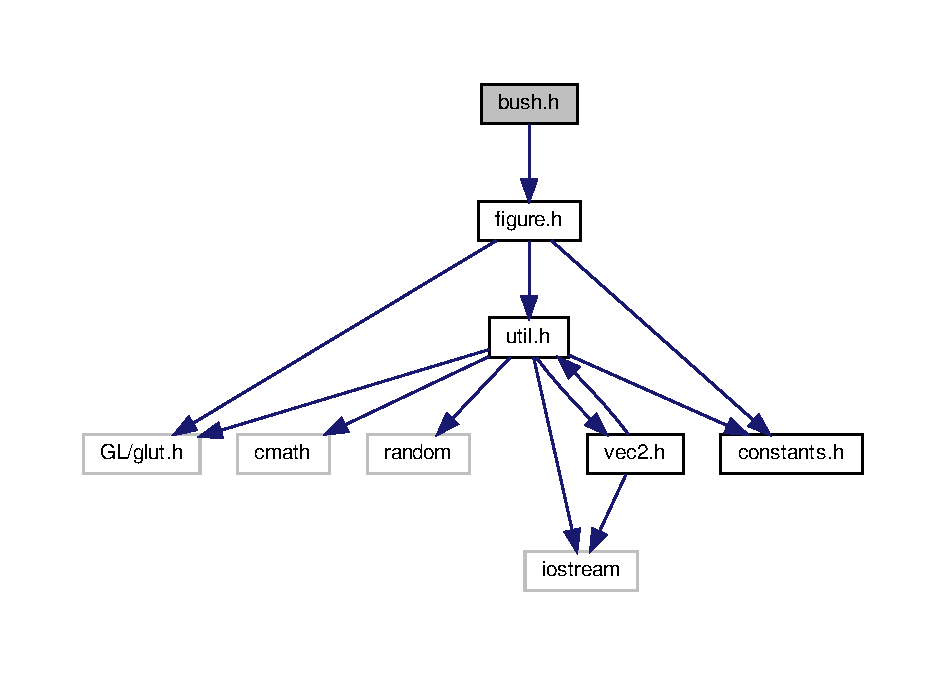
\includegraphics[width=350pt]{dc/d28/bush_8h__incl}
\end{center}
\end{figure}
This graph shows which files directly or indirectly include this file\+:
\nopagebreak
\begin{figure}[H]
\begin{center}
\leavevmode
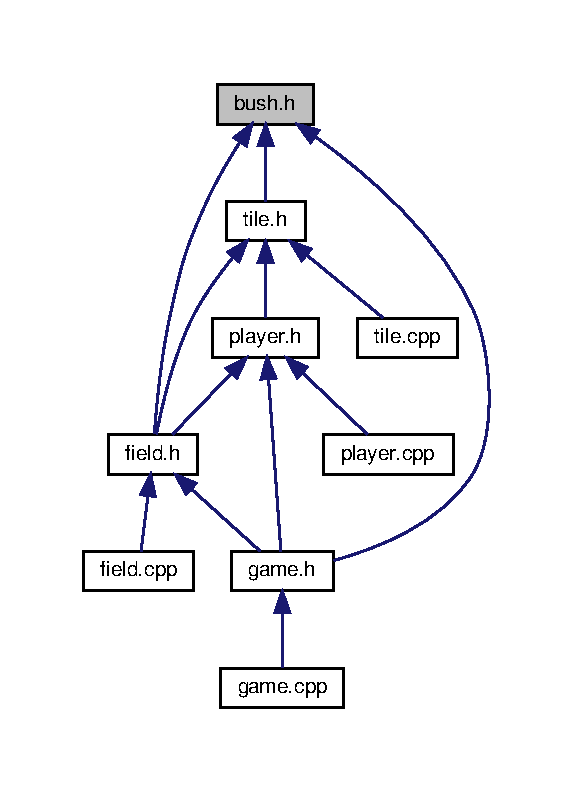
\includegraphics[width=288pt]{d6/d39/bush_8h__dep__incl}
\end{center}
\end{figure}
\subsection*{Classes}
\begin{DoxyCompactItemize}
\item 
class \hyperlink{classBush}{Bush}
\end{DoxyCompactItemize}

\hypertarget{coin_8h}{}\section{coin.\+h File Reference}
\label{coin_8h}\index{coin.\+h@{coin.\+h}}
{\ttfamily \#include \char`\"{}figure.\+h\char`\"{}}\newline
Include dependency graph for coin.\+h\+:
\nopagebreak
\begin{figure}[H]
\begin{center}
\leavevmode
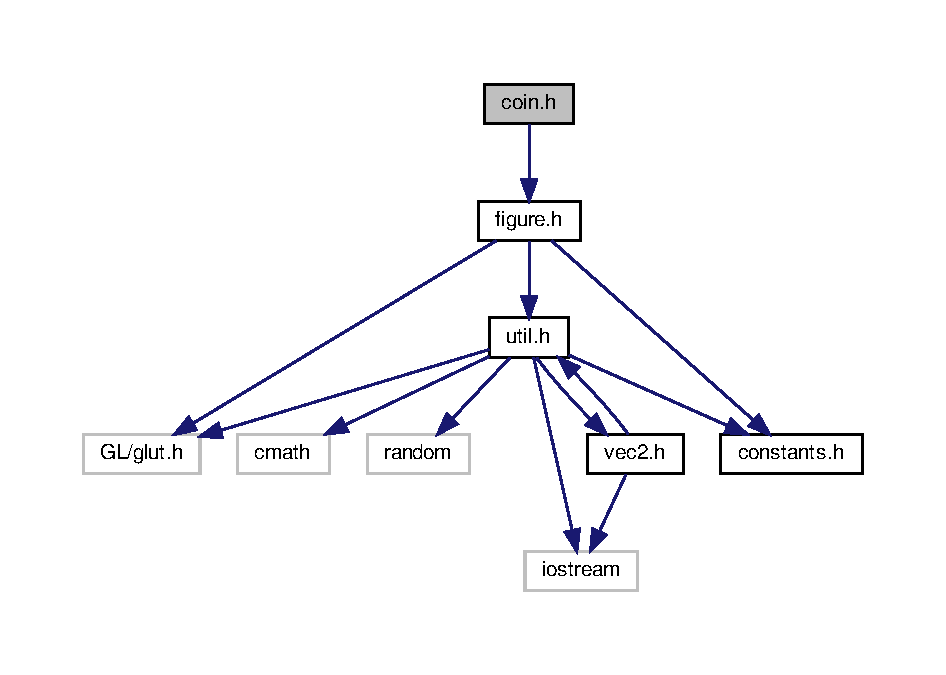
\includegraphics[width=350pt]{de/dbc/coin_8h__incl}
\end{center}
\end{figure}
This graph shows which files directly or indirectly include this file\+:
\nopagebreak
\begin{figure}[H]
\begin{center}
\leavevmode
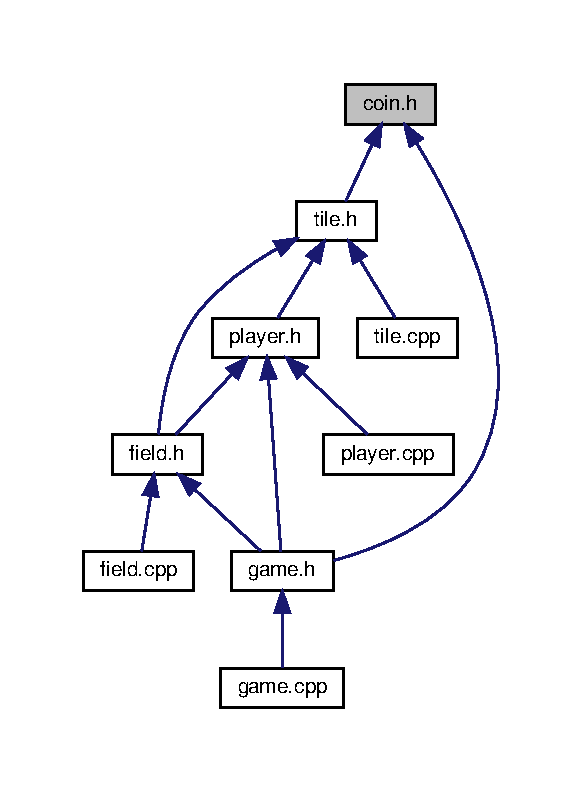
\includegraphics[width=316pt]{d3/d33/coin_8h__dep__incl}
\end{center}
\end{figure}
\subsection*{Classes}
\begin{DoxyCompactItemize}
\item 
class \hyperlink{classCoin}{Coin}
\end{DoxyCompactItemize}

\hypertarget{color_8h}{}\section{color.\+h File Reference}
\label{color_8h}\index{color.\+h@{color.\+h}}
This graph shows which files directly or indirectly include this file\+:
\nopagebreak
\begin{figure}[H]
\begin{center}
\leavevmode
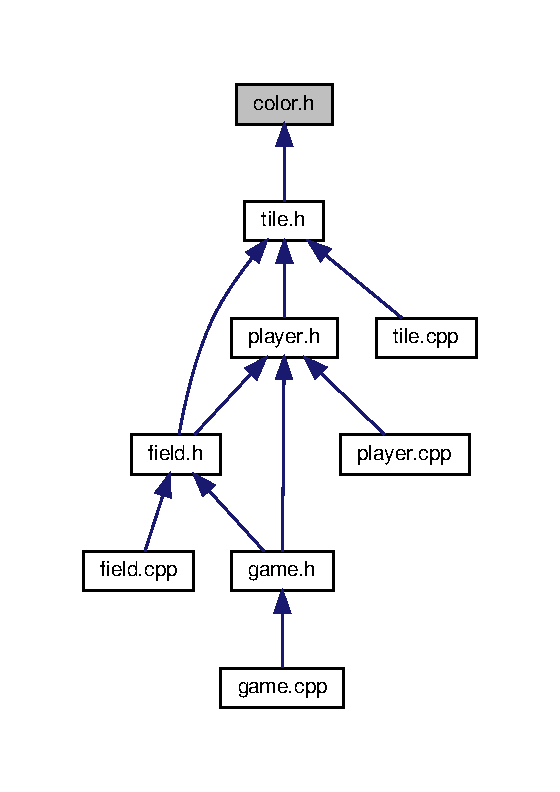
\includegraphics[width=269pt]{da/d0a/color_8h__dep__incl}
\end{center}
\end{figure}
\subsection*{Classes}
\begin{DoxyCompactItemize}
\item 
struct \hyperlink{structColor}{Color}
\end{DoxyCompactItemize}

\hypertarget{constants_8h}{}\section{constants.\+h File Reference}
\label{constants_8h}\index{constants.\+h@{constants.\+h}}
This graph shows which files directly or indirectly include this file\+:
\nopagebreak
\begin{figure}[H]
\begin{center}
\leavevmode
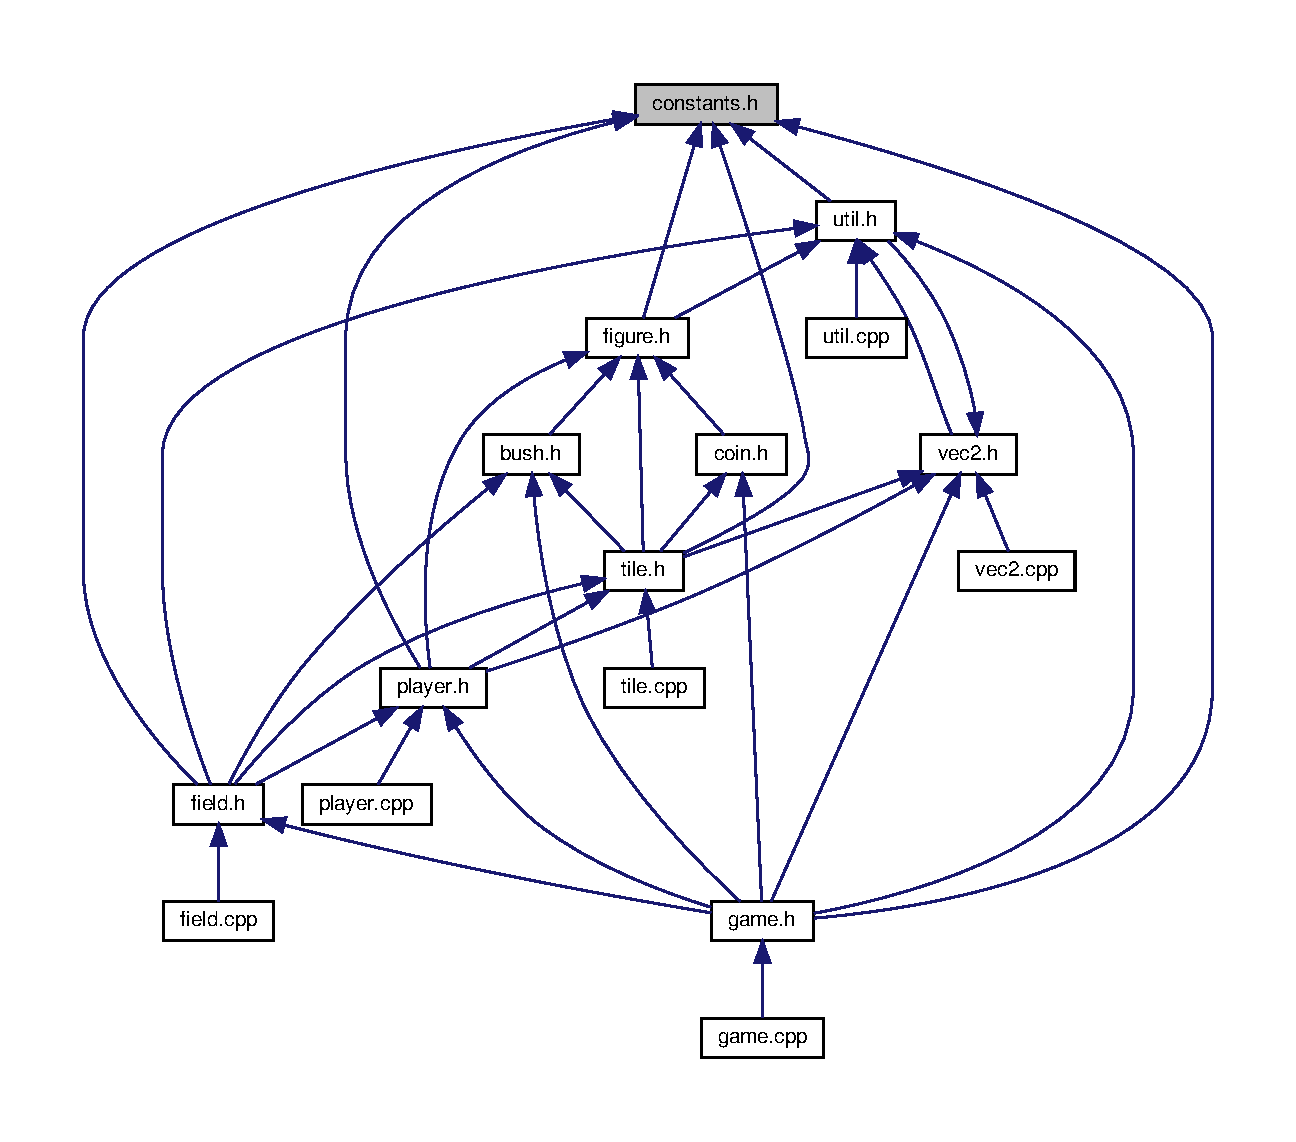
\includegraphics[width=350pt]{dd/d0e/constants_8h__dep__incl}
\end{center}
\end{figure}
\subsection*{Macros}
\begin{DoxyCompactItemize}
\item 
\#define \hyperlink{constants_8h_a1cc42d50f23486ba30cb2f366bf409c2}{T\+U\+R\+N\+\_\+\+W\+A\+L\+K\+I\+N\+G\+\_\+\+D\+I\+S\+T\+A\+N\+CE}~5
\item 
\#define \hyperlink{constants_8h_a0faca545c24d19a478358a4fe7c7ec85}{T\+I\+L\+E\+\_\+\+S\+T\+E\+P\+\_\+\+H\+E\+I\+G\+HT}~0.\+15f
\item 
\#define \hyperlink{constants_8h_a3ca0b8b8bc919598c498f0a78faa0af6}{P\+A\+T\+H\+\_\+\+H\+E\+I\+G\+H\+T\+\_\+\+D\+I\+S\+C\+R\+E\+P\+A\+N\+CY}~3
\item 
\#define \hyperlink{constants_8h_a002b2f4894492820fe708b1b7e7c5e70}{E\+P\+S\+I\+L\+ON}~0.\+00001f
\item 
\#define \hyperlink{constants_8h_a598a3330b3c21701223ee0ca14316eca}{PI}~3.\+14159f
\item 
\#define \hyperlink{constants_8h_aebad45bfa06a5d66805c5813fbc59f4b}{I\+N\+V\+\_\+\+PI}~0.\+31831f
\item 
\#define \hyperlink{constants_8h_a2203853edabc3de5f785e54b55eb5e3c}{P\+HI}~2.\+39996f
\item 
\#define \hyperlink{constants_8h_aa99ab3cf63c47fc110df80ffc8081898}{three\+\_\+sqrt\+\_\+half}~0.\+86602f
\item 
\#define \hyperlink{constants_8h_a1c8eabf8f78d1052303a7e828747aea6}{three\+\_\+sqrt\+\_\+half\+\_\+inv}~1.\+15470f
\item 
\#define \hyperlink{constants_8h_aefc27696c4e811fe78476e21a5fb184d}{hexagon\+\_\+area}~2.\+59808f
\end{DoxyCompactItemize}


\subsection{Macro Definition Documentation}
\mbox{\Hypertarget{constants_8h_a002b2f4894492820fe708b1b7e7c5e70}\label{constants_8h_a002b2f4894492820fe708b1b7e7c5e70}} 
\index{constants.\+h@{constants.\+h}!E\+P\+S\+I\+L\+ON@{E\+P\+S\+I\+L\+ON}}
\index{E\+P\+S\+I\+L\+ON@{E\+P\+S\+I\+L\+ON}!constants.\+h@{constants.\+h}}
\subsubsection{\texorpdfstring{E\+P\+S\+I\+L\+ON}{EPSILON}}
{\footnotesize\ttfamily \#define E\+P\+S\+I\+L\+ON~0.\+00001f}

\mbox{\Hypertarget{constants_8h_aefc27696c4e811fe78476e21a5fb184d}\label{constants_8h_aefc27696c4e811fe78476e21a5fb184d}} 
\index{constants.\+h@{constants.\+h}!hexagon\+\_\+area@{hexagon\+\_\+area}}
\index{hexagon\+\_\+area@{hexagon\+\_\+area}!constants.\+h@{constants.\+h}}
\subsubsection{\texorpdfstring{hexagon\+\_\+area}{hexagon\_area}}
{\footnotesize\ttfamily \#define hexagon\+\_\+area~2.\+59808f}

\mbox{\Hypertarget{constants_8h_aebad45bfa06a5d66805c5813fbc59f4b}\label{constants_8h_aebad45bfa06a5d66805c5813fbc59f4b}} 
\index{constants.\+h@{constants.\+h}!I\+N\+V\+\_\+\+PI@{I\+N\+V\+\_\+\+PI}}
\index{I\+N\+V\+\_\+\+PI@{I\+N\+V\+\_\+\+PI}!constants.\+h@{constants.\+h}}
\subsubsection{\texorpdfstring{I\+N\+V\+\_\+\+PI}{INV\_PI}}
{\footnotesize\ttfamily \#define I\+N\+V\+\_\+\+PI~0.\+31831f}

\mbox{\Hypertarget{constants_8h_a3ca0b8b8bc919598c498f0a78faa0af6}\label{constants_8h_a3ca0b8b8bc919598c498f0a78faa0af6}} 
\index{constants.\+h@{constants.\+h}!P\+A\+T\+H\+\_\+\+H\+E\+I\+G\+H\+T\+\_\+\+D\+I\+S\+C\+R\+E\+P\+A\+N\+CY@{P\+A\+T\+H\+\_\+\+H\+E\+I\+G\+H\+T\+\_\+\+D\+I\+S\+C\+R\+E\+P\+A\+N\+CY}}
\index{P\+A\+T\+H\+\_\+\+H\+E\+I\+G\+H\+T\+\_\+\+D\+I\+S\+C\+R\+E\+P\+A\+N\+CY@{P\+A\+T\+H\+\_\+\+H\+E\+I\+G\+H\+T\+\_\+\+D\+I\+S\+C\+R\+E\+P\+A\+N\+CY}!constants.\+h@{constants.\+h}}
\subsubsection{\texorpdfstring{P\+A\+T\+H\+\_\+\+H\+E\+I\+G\+H\+T\+\_\+\+D\+I\+S\+C\+R\+E\+P\+A\+N\+CY}{PATH\_HEIGHT\_DISCREPANCY}}
{\footnotesize\ttfamily \#define P\+A\+T\+H\+\_\+\+H\+E\+I\+G\+H\+T\+\_\+\+D\+I\+S\+C\+R\+E\+P\+A\+N\+CY~3}

\mbox{\Hypertarget{constants_8h_a2203853edabc3de5f785e54b55eb5e3c}\label{constants_8h_a2203853edabc3de5f785e54b55eb5e3c}} 
\index{constants.\+h@{constants.\+h}!P\+HI@{P\+HI}}
\index{P\+HI@{P\+HI}!constants.\+h@{constants.\+h}}
\subsubsection{\texorpdfstring{P\+HI}{PHI}}
{\footnotesize\ttfamily \#define P\+HI~2.\+39996f}

\mbox{\Hypertarget{constants_8h_a598a3330b3c21701223ee0ca14316eca}\label{constants_8h_a598a3330b3c21701223ee0ca14316eca}} 
\index{constants.\+h@{constants.\+h}!PI@{PI}}
\index{PI@{PI}!constants.\+h@{constants.\+h}}
\subsubsection{\texorpdfstring{PI}{PI}}
{\footnotesize\ttfamily \#define PI~3.\+14159f}

\mbox{\Hypertarget{constants_8h_aa99ab3cf63c47fc110df80ffc8081898}\label{constants_8h_aa99ab3cf63c47fc110df80ffc8081898}} 
\index{constants.\+h@{constants.\+h}!three\+\_\+sqrt\+\_\+half@{three\+\_\+sqrt\+\_\+half}}
\index{three\+\_\+sqrt\+\_\+half@{three\+\_\+sqrt\+\_\+half}!constants.\+h@{constants.\+h}}
\subsubsection{\texorpdfstring{three\+\_\+sqrt\+\_\+half}{three\_sqrt\_half}}
{\footnotesize\ttfamily \#define three\+\_\+sqrt\+\_\+half~0.\+86602f}

\mbox{\Hypertarget{constants_8h_a1c8eabf8f78d1052303a7e828747aea6}\label{constants_8h_a1c8eabf8f78d1052303a7e828747aea6}} 
\index{constants.\+h@{constants.\+h}!three\+\_\+sqrt\+\_\+half\+\_\+inv@{three\+\_\+sqrt\+\_\+half\+\_\+inv}}
\index{three\+\_\+sqrt\+\_\+half\+\_\+inv@{three\+\_\+sqrt\+\_\+half\+\_\+inv}!constants.\+h@{constants.\+h}}
\subsubsection{\texorpdfstring{three\+\_\+sqrt\+\_\+half\+\_\+inv}{three\_sqrt\_half\_inv}}
{\footnotesize\ttfamily \#define three\+\_\+sqrt\+\_\+half\+\_\+inv~1.\+15470f}

\mbox{\Hypertarget{constants_8h_a0faca545c24d19a478358a4fe7c7ec85}\label{constants_8h_a0faca545c24d19a478358a4fe7c7ec85}} 
\index{constants.\+h@{constants.\+h}!T\+I\+L\+E\+\_\+\+S\+T\+E\+P\+\_\+\+H\+E\+I\+G\+HT@{T\+I\+L\+E\+\_\+\+S\+T\+E\+P\+\_\+\+H\+E\+I\+G\+HT}}
\index{T\+I\+L\+E\+\_\+\+S\+T\+E\+P\+\_\+\+H\+E\+I\+G\+HT@{T\+I\+L\+E\+\_\+\+S\+T\+E\+P\+\_\+\+H\+E\+I\+G\+HT}!constants.\+h@{constants.\+h}}
\subsubsection{\texorpdfstring{T\+I\+L\+E\+\_\+\+S\+T\+E\+P\+\_\+\+H\+E\+I\+G\+HT}{TILE\_STEP\_HEIGHT}}
{\footnotesize\ttfamily \#define T\+I\+L\+E\+\_\+\+S\+T\+E\+P\+\_\+\+H\+E\+I\+G\+HT~0.\+15f}

\mbox{\Hypertarget{constants_8h_a1cc42d50f23486ba30cb2f366bf409c2}\label{constants_8h_a1cc42d50f23486ba30cb2f366bf409c2}} 
\index{constants.\+h@{constants.\+h}!T\+U\+R\+N\+\_\+\+W\+A\+L\+K\+I\+N\+G\+\_\+\+D\+I\+S\+T\+A\+N\+CE@{T\+U\+R\+N\+\_\+\+W\+A\+L\+K\+I\+N\+G\+\_\+\+D\+I\+S\+T\+A\+N\+CE}}
\index{T\+U\+R\+N\+\_\+\+W\+A\+L\+K\+I\+N\+G\+\_\+\+D\+I\+S\+T\+A\+N\+CE@{T\+U\+R\+N\+\_\+\+W\+A\+L\+K\+I\+N\+G\+\_\+\+D\+I\+S\+T\+A\+N\+CE}!constants.\+h@{constants.\+h}}
\subsubsection{\texorpdfstring{T\+U\+R\+N\+\_\+\+W\+A\+L\+K\+I\+N\+G\+\_\+\+D\+I\+S\+T\+A\+N\+CE}{TURN\_WALKING\_DISTANCE}}
{\footnotesize\ttfamily \#define T\+U\+R\+N\+\_\+\+W\+A\+L\+K\+I\+N\+G\+\_\+\+D\+I\+S\+T\+A\+N\+CE~5}


\hypertarget{field_8cpp}{}\section{field.\+cpp File Reference}
\label{field_8cpp}\index{field.\+cpp@{field.\+cpp}}
{\ttfamily \#include \char`\"{}field.\+h\char`\"{}}\newline
Include dependency graph for field.\+cpp\+:
\nopagebreak
\begin{figure}[H]
\begin{center}
\leavevmode
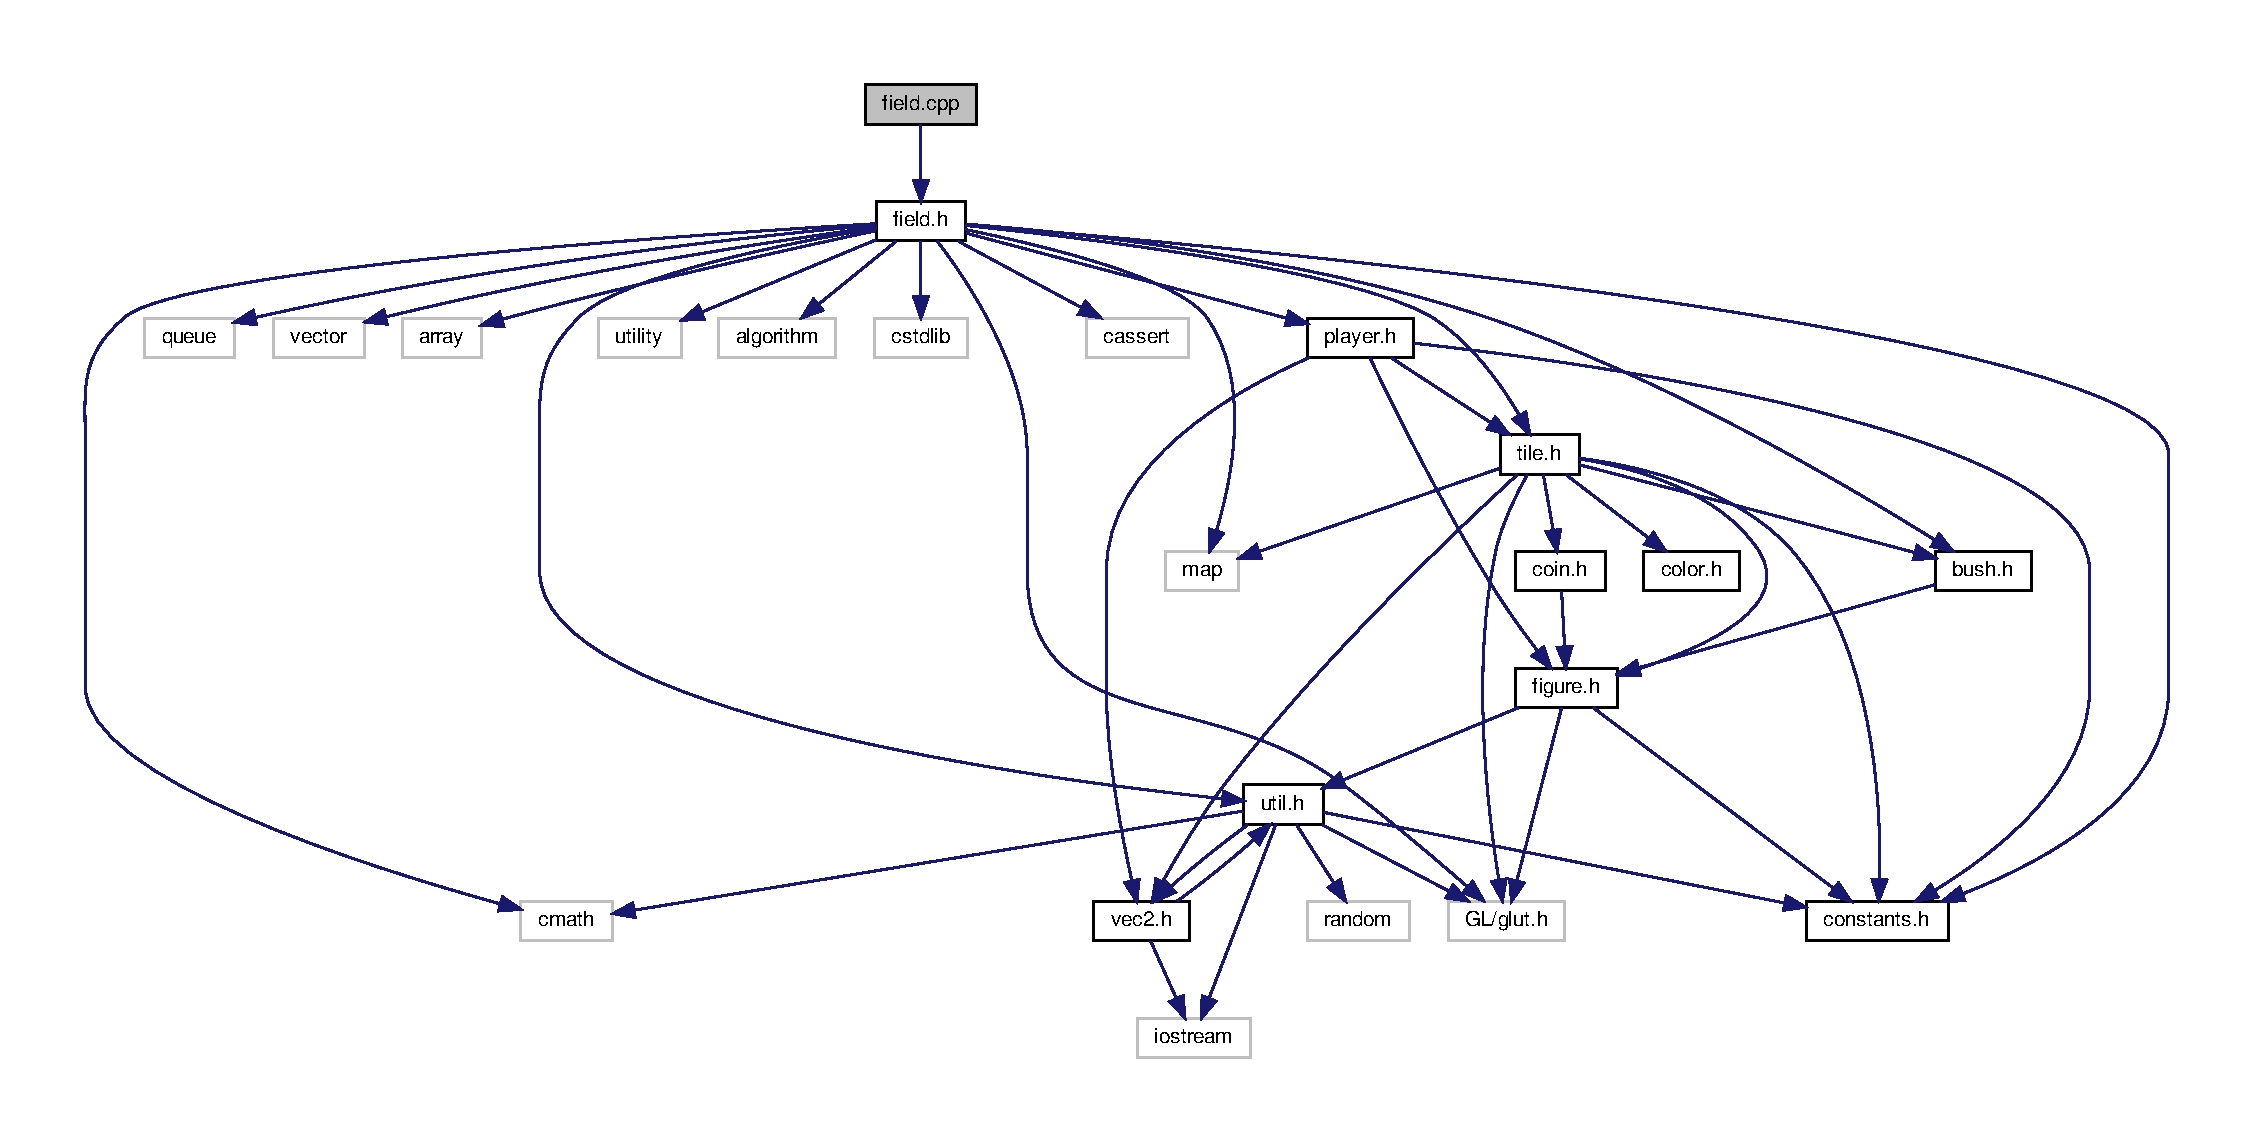
\includegraphics[width=350pt]{d0/d9a/field_8cpp__incl}
\end{center}
\end{figure}

\hypertarget{field_8h}{}\section{field.\+h File Reference}
\label{field_8h}\index{field.\+h@{field.\+h}}
{\ttfamily \#include $<$G\+L/glut.\+h$>$}\newline
{\ttfamily \#include $<$queue$>$}\newline
{\ttfamily \#include $<$vector$>$}\newline
{\ttfamily \#include $<$array$>$}\newline
{\ttfamily \#include $<$map$>$}\newline
{\ttfamily \#include $<$utility$>$}\newline
{\ttfamily \#include $<$algorithm$>$}\newline
{\ttfamily \#include $<$cstdlib$>$}\newline
{\ttfamily \#include $<$cmath$>$}\newline
{\ttfamily \#include $<$cassert$>$}\newline
{\ttfamily \#include \char`\"{}constants.\+h\char`\"{}}\newline
{\ttfamily \#include \char`\"{}tile.\+h\char`\"{}}\newline
{\ttfamily \#include \char`\"{}bush.\+h\char`\"{}}\newline
{\ttfamily \#include \char`\"{}util.\+h\char`\"{}}\newline
{\ttfamily \#include \char`\"{}player.\+h\char`\"{}}\newline
Include dependency graph for field.\+h\+:
\nopagebreak
\begin{figure}[H]
\begin{center}
\leavevmode
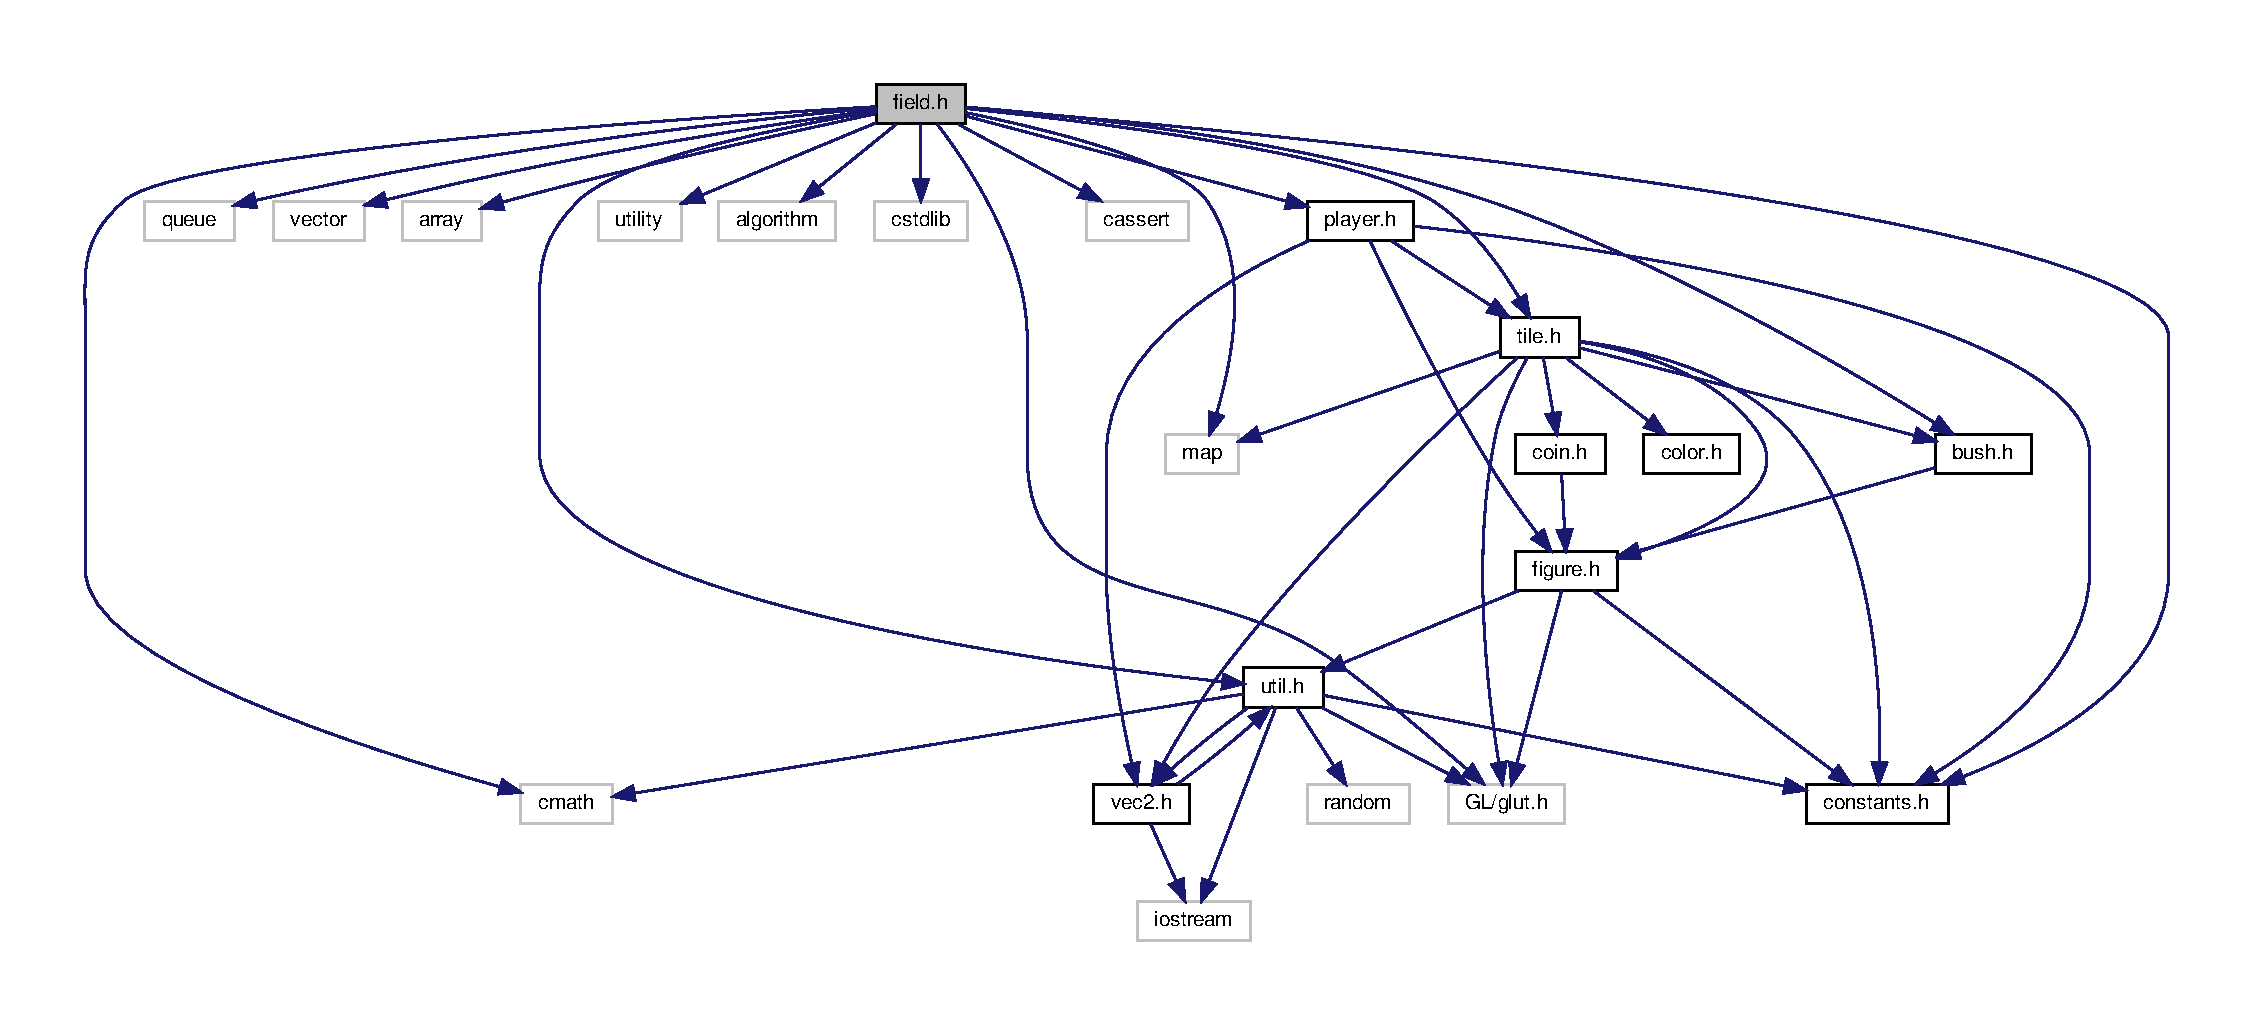
\includegraphics[width=350pt]{d7/d64/field_8h__incl}
\end{center}
\end{figure}
This graph shows which files directly or indirectly include this file\+:
\nopagebreak
\begin{figure}[H]
\begin{center}
\leavevmode
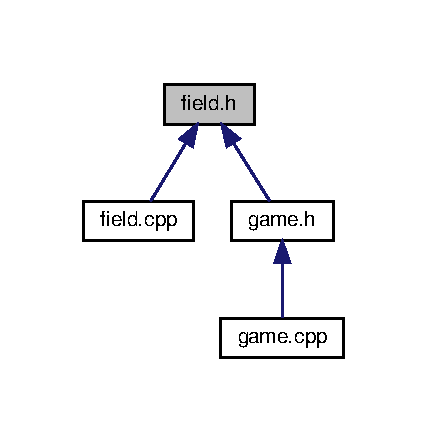
\includegraphics[width=205pt]{d6/d8f/field_8h__dep__incl}
\end{center}
\end{figure}
\subsection*{Classes}
\begin{DoxyCompactItemize}
\item 
class \hyperlink{classField}{Field}
\end{DoxyCompactItemize}

\hypertarget{figure_8h}{}\section{figure.\+h File Reference}
\label{figure_8h}\index{figure.\+h@{figure.\+h}}
{\ttfamily \#include $<$G\+L/glut.\+h$>$}\newline
{\ttfamily \#include \char`\"{}util.\+h\char`\"{}}\newline
{\ttfamily \#include \char`\"{}constants.\+h\char`\"{}}\newline
Include dependency graph for figure.\+h\+:
\nopagebreak
\begin{figure}[H]
\begin{center}
\leavevmode
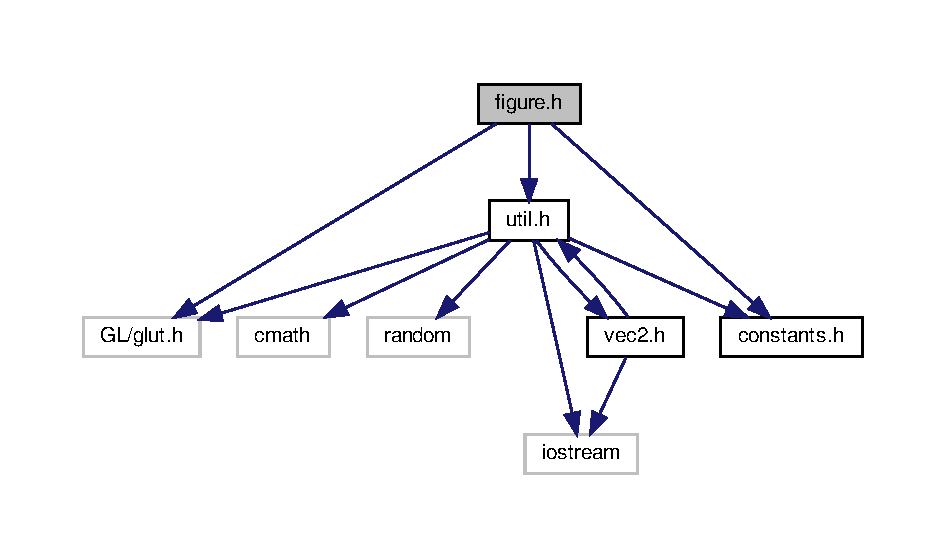
\includegraphics[width=350pt]{d9/df1/figure_8h__incl}
\end{center}
\end{figure}
This graph shows which files directly or indirectly include this file\+:
\nopagebreak
\begin{figure}[H]
\begin{center}
\leavevmode
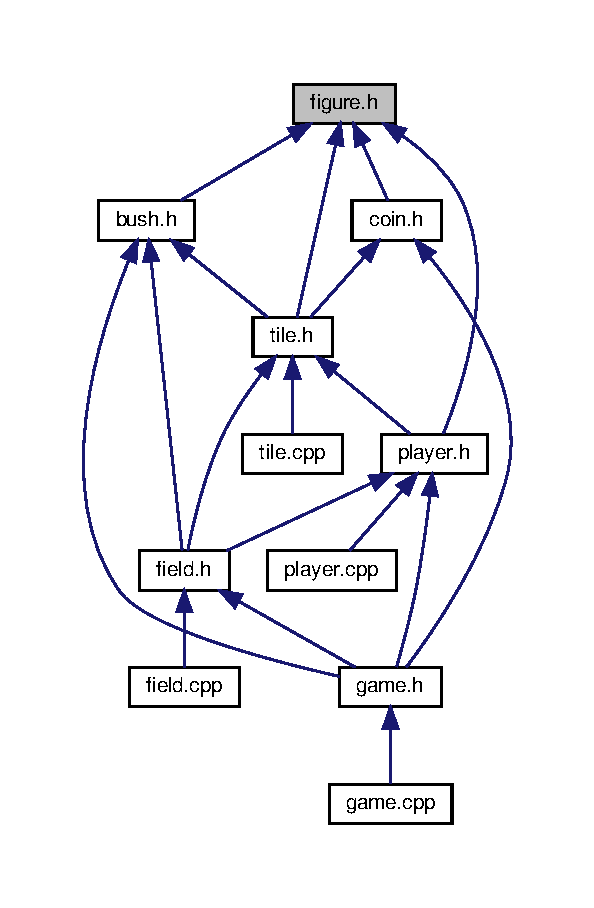
\includegraphics[width=285pt]{d8/db1/figure_8h__dep__incl}
\end{center}
\end{figure}
\subsection*{Classes}
\begin{DoxyCompactItemize}
\item 
class \hyperlink{classFigure}{Figure}
\end{DoxyCompactItemize}

\hypertarget{game_8cpp}{}\section{game.\+cpp File Reference}
\label{game_8cpp}\index{game.\+cpp@{game.\+cpp}}
{\ttfamily \#include \char`\"{}game.\+h\char`\"{}}\newline
Include dependency graph for game.\+cpp\+:
\nopagebreak
\begin{figure}[H]
\begin{center}
\leavevmode
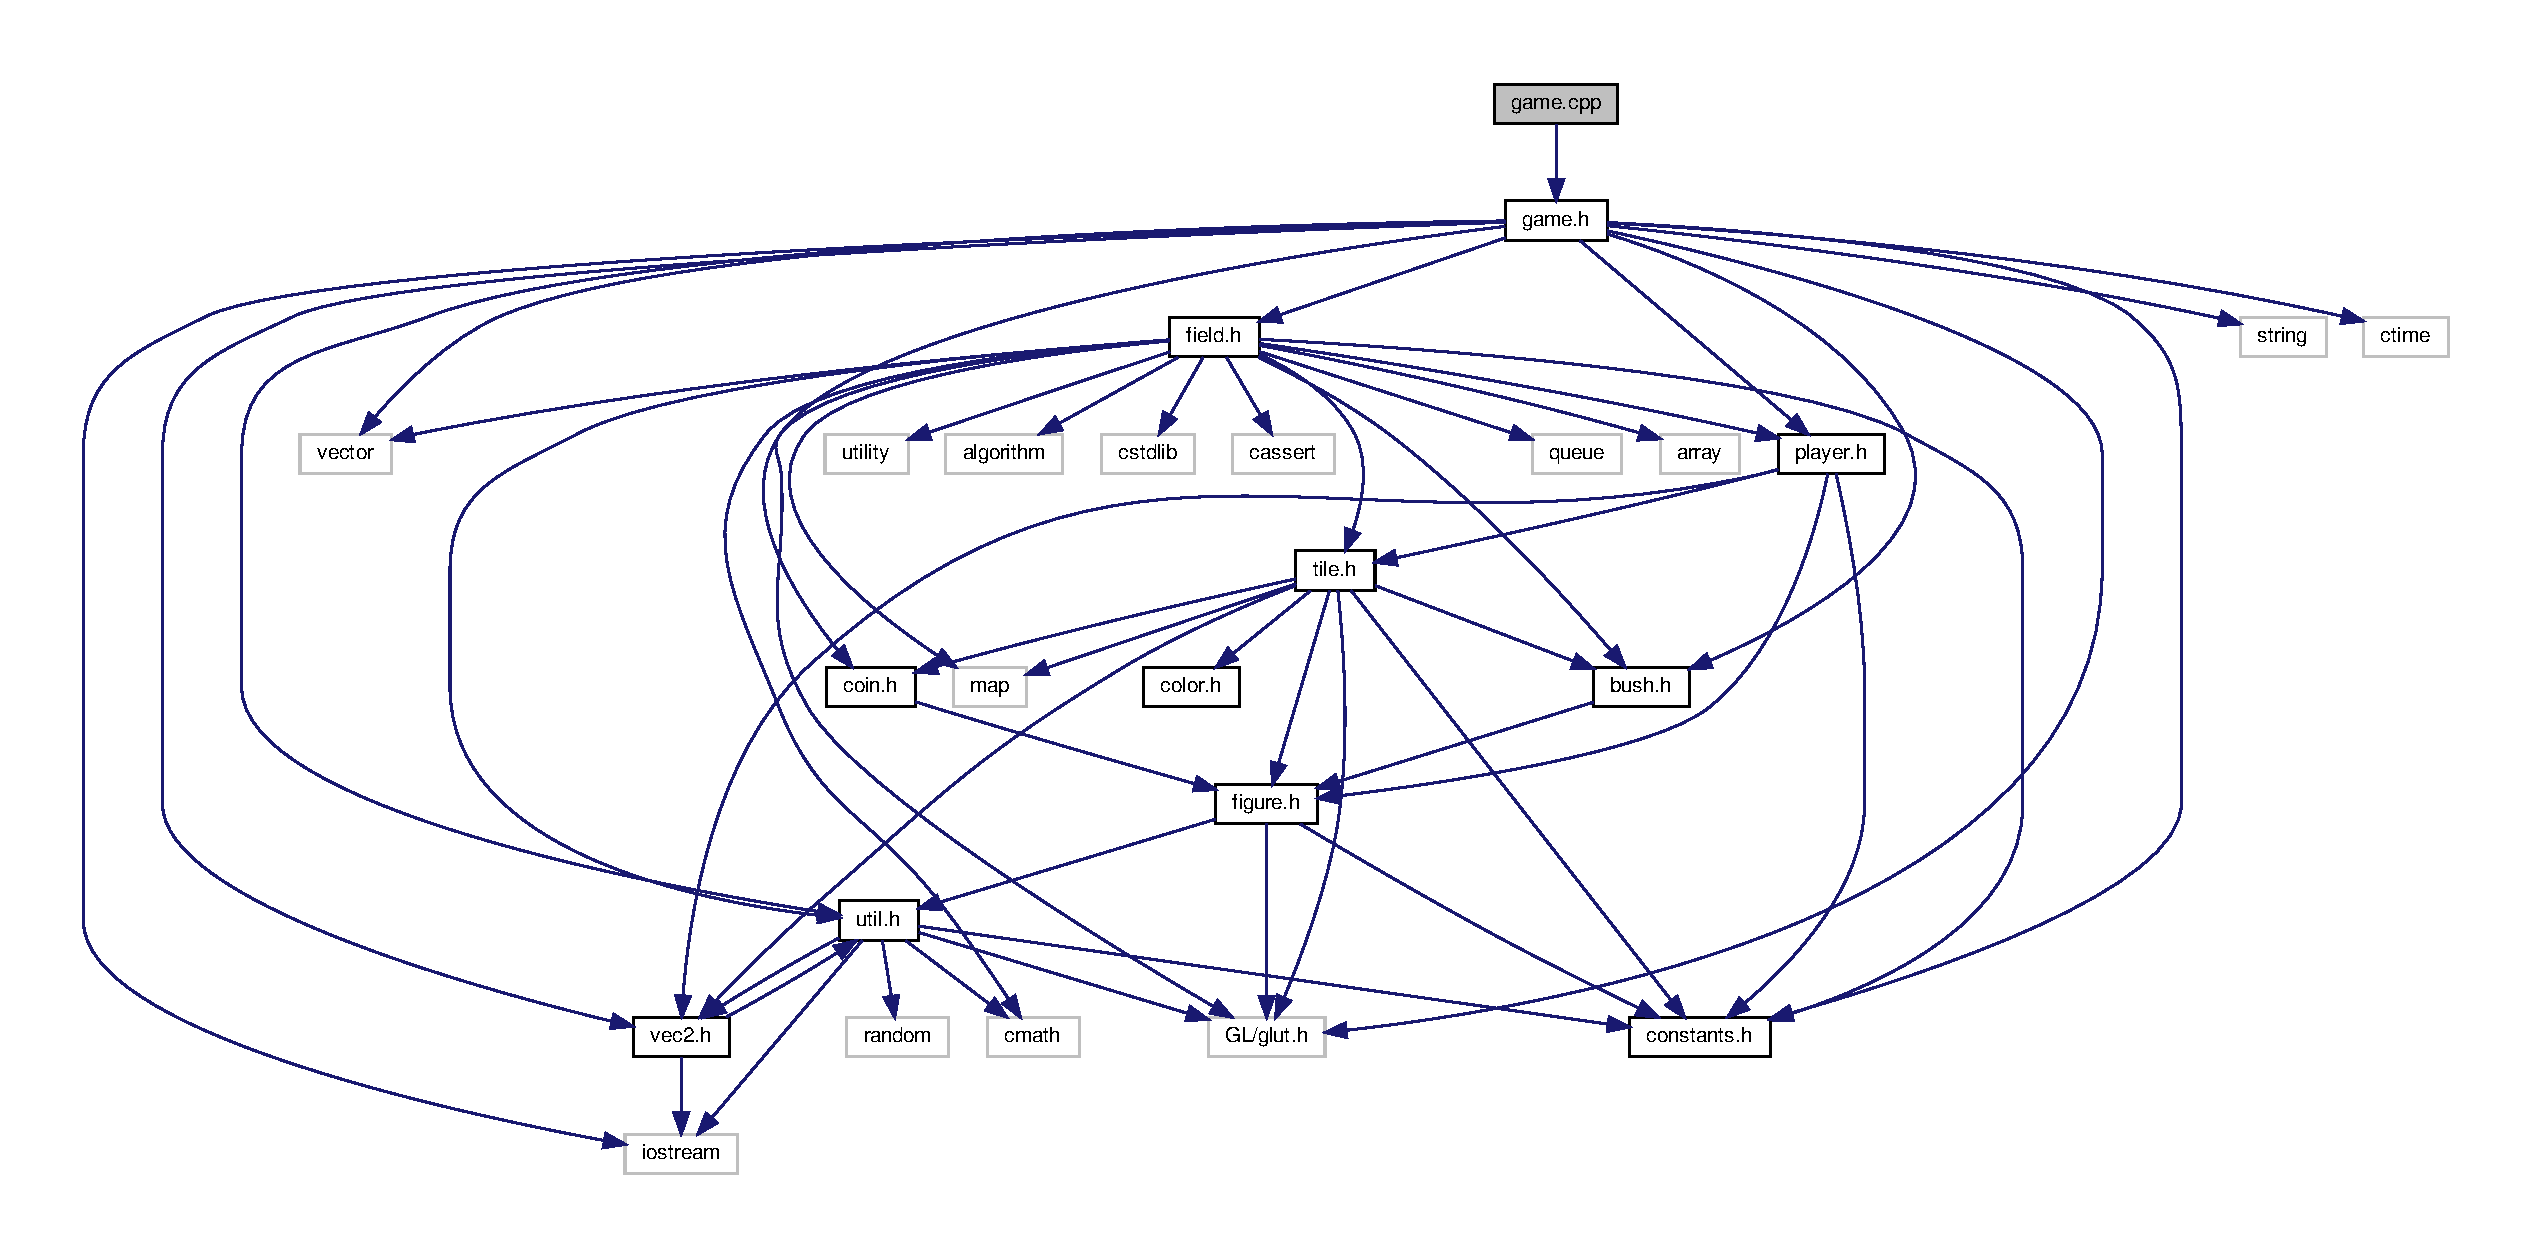
\includegraphics[width=350pt]{dd/dbf/game_8cpp__incl}
\end{center}
\end{figure}
\subsection*{Functions}
\begin{DoxyCompactItemize}
\item 
int \hyperlink{game_8cpp_a3c04138a5bfe5d72780bb7e82a18e627}{main} (int argc, char $\ast$$\ast$argv)
\end{DoxyCompactItemize}


\subsection{Function Documentation}
\mbox{\Hypertarget{game_8cpp_a3c04138a5bfe5d72780bb7e82a18e627}\label{game_8cpp_a3c04138a5bfe5d72780bb7e82a18e627}} 
\index{game.\+cpp@{game.\+cpp}!main@{main}}
\index{main@{main}!game.\+cpp@{game.\+cpp}}
\subsubsection{\texorpdfstring{main()}{main()}}
{\footnotesize\ttfamily int main (\begin{DoxyParamCaption}\item[{int}]{argc,  }\item[{char $\ast$$\ast$}]{argv }\end{DoxyParamCaption})}


\hypertarget{game_8h}{}\section{game.\+h File Reference}
\label{game_8h}\index{game.\+h@{game.\+h}}
{\ttfamily \#include $<$G\+L/glut.\+h$>$}\newline
{\ttfamily \#include $<$iostream$>$}\newline
{\ttfamily \#include $<$vector$>$}\newline
{\ttfamily \#include $<$string$>$}\newline
{\ttfamily \#include $<$ctime$>$}\newline
{\ttfamily \#include \char`\"{}constants.\+h\char`\"{}}\newline
{\ttfamily \#include \char`\"{}util.\+h\char`\"{}}\newline
{\ttfamily \#include \char`\"{}vec2.\+h\char`\"{}}\newline
{\ttfamily \#include \char`\"{}field.\+h\char`\"{}}\newline
{\ttfamily \#include \char`\"{}player.\+h\char`\"{}}\newline
{\ttfamily \#include \char`\"{}coin.\+h\char`\"{}}\newline
{\ttfamily \#include \char`\"{}bush.\+h\char`\"{}}\newline
Include dependency graph for game.\+h\+:
\nopagebreak
\begin{figure}[H]
\begin{center}
\leavevmode
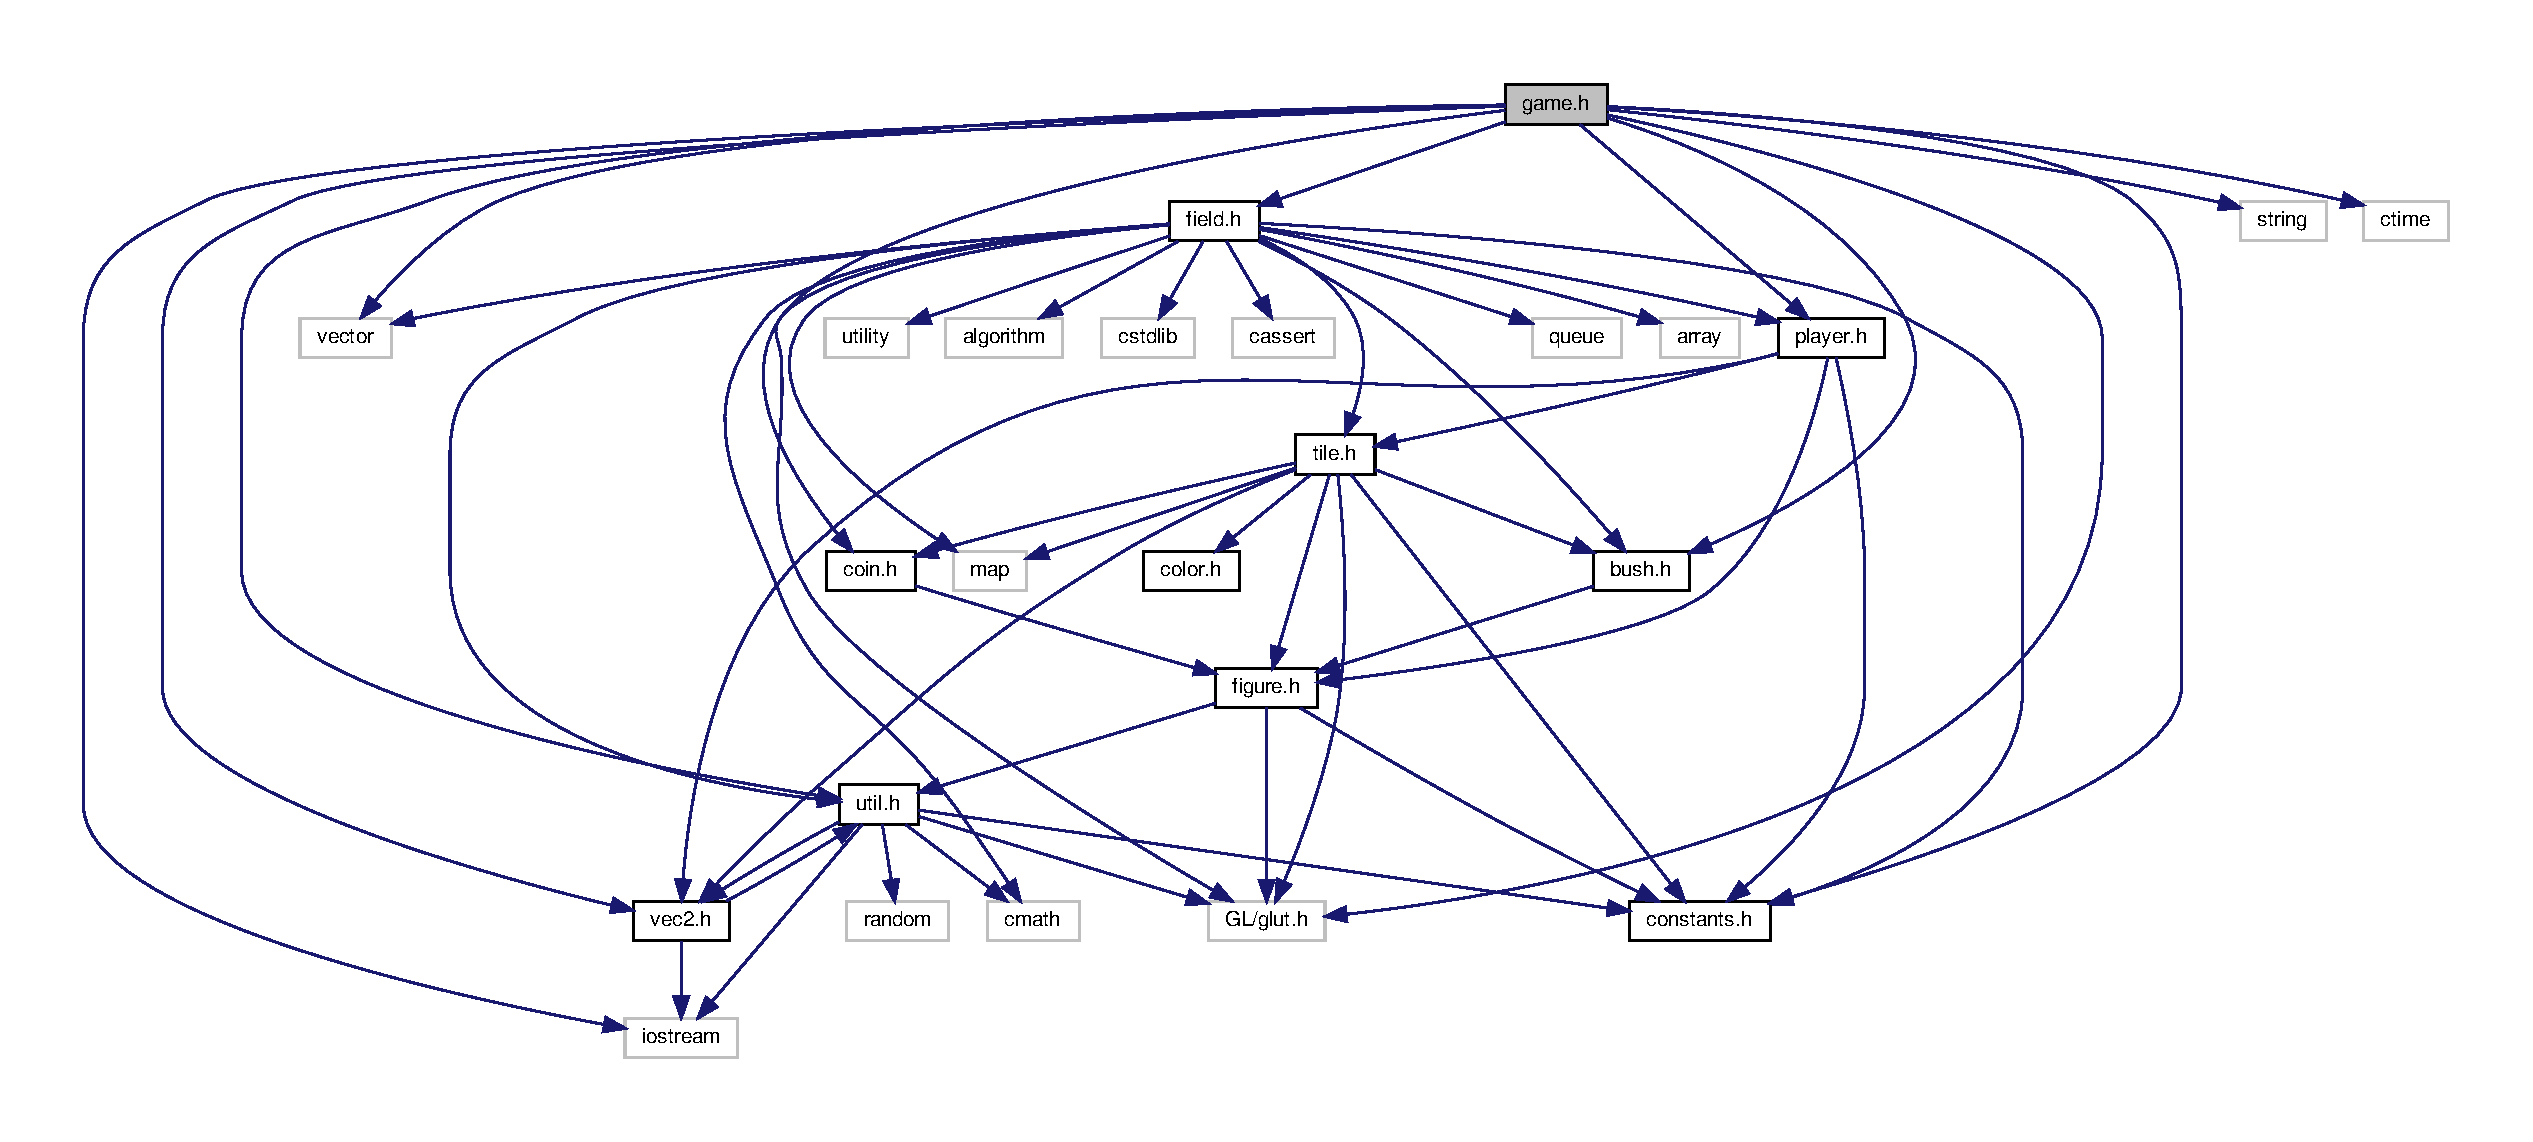
\includegraphics[width=350pt]{d1/d10/game_8h__incl}
\end{center}
\end{figure}
This graph shows which files directly or indirectly include this file\+:
\nopagebreak
\begin{figure}[H]
\begin{center}
\leavevmode
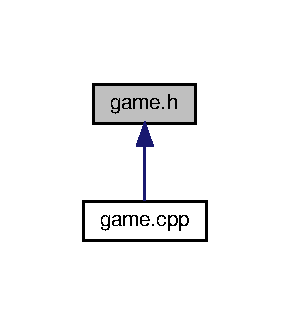
\includegraphics[width=139pt]{df/dcc/game_8h__dep__incl}
\end{center}
\end{figure}
\subsection*{Classes}
\begin{DoxyCompactItemize}
\item 
class \hyperlink{classGame}{Game}
\end{DoxyCompactItemize}
\subsection*{Functions}
\begin{DoxyCompactItemize}
\item 
void \hyperlink{game_8h_a612f315a95cd727d49d9699ded494efa}{draw\+Callback} ()
\item 
void \hyperlink{game_8h_a11eb900902ba49145d19defcf4b164c0}{mouse\+Callback} (int button, int state, int x, int y)
\item 
void \hyperlink{game_8h_aac26d635daf1ca3864d0f5372073dbfa}{mousemotion\+Callback} (int x, int y)
\item 
void \hyperlink{game_8h_a0ad6379206023c2b36121fe612642fe1}{passivmotion\+Callback} (int x, int y)
\item 
void \hyperlink{game_8h_a566b1f01cbd792b5ffebc32509dd311e}{keyboard\+Callback} (unsigned char c, int x, int y)
\item 
void \hyperlink{game_8h_af7691aeec7899f251182101f2a6443f8}{reshape\+Callback} (int width, int height)
\item 
int \hyperlink{game_8h_a3c04138a5bfe5d72780bb7e82a18e627}{main} (int argc, char $\ast$$\ast$argv)
\end{DoxyCompactItemize}


\subsection{Function Documentation}
\mbox{\Hypertarget{game_8h_a612f315a95cd727d49d9699ded494efa}\label{game_8h_a612f315a95cd727d49d9699ded494efa}} 
\index{game.\+h@{game.\+h}!draw\+Callback@{draw\+Callback}}
\index{draw\+Callback@{draw\+Callback}!game.\+h@{game.\+h}}
\subsubsection{\texorpdfstring{draw\+Callback()}{drawCallback()}}
{\footnotesize\ttfamily void draw\+Callback (\begin{DoxyParamCaption}{ }\end{DoxyParamCaption})\hspace{0.3cm}{\ttfamily [inline]}}

\mbox{\Hypertarget{game_8h_a566b1f01cbd792b5ffebc32509dd311e}\label{game_8h_a566b1f01cbd792b5ffebc32509dd311e}} 
\index{game.\+h@{game.\+h}!keyboard\+Callback@{keyboard\+Callback}}
\index{keyboard\+Callback@{keyboard\+Callback}!game.\+h@{game.\+h}}
\subsubsection{\texorpdfstring{keyboard\+Callback()}{keyboardCallback()}}
{\footnotesize\ttfamily void keyboard\+Callback (\begin{DoxyParamCaption}\item[{unsigned char}]{c,  }\item[{int}]{x,  }\item[{int}]{y }\end{DoxyParamCaption})\hspace{0.3cm}{\ttfamily [inline]}}

\mbox{\Hypertarget{game_8h_a3c04138a5bfe5d72780bb7e82a18e627}\label{game_8h_a3c04138a5bfe5d72780bb7e82a18e627}} 
\index{game.\+h@{game.\+h}!main@{main}}
\index{main@{main}!game.\+h@{game.\+h}}
\subsubsection{\texorpdfstring{main()}{main()}}
{\footnotesize\ttfamily int main (\begin{DoxyParamCaption}\item[{int}]{argc,  }\item[{char $\ast$$\ast$}]{argv }\end{DoxyParamCaption})}

\mbox{\Hypertarget{game_8h_a11eb900902ba49145d19defcf4b164c0}\label{game_8h_a11eb900902ba49145d19defcf4b164c0}} 
\index{game.\+h@{game.\+h}!mouse\+Callback@{mouse\+Callback}}
\index{mouse\+Callback@{mouse\+Callback}!game.\+h@{game.\+h}}
\subsubsection{\texorpdfstring{mouse\+Callback()}{mouseCallback()}}
{\footnotesize\ttfamily void mouse\+Callback (\begin{DoxyParamCaption}\item[{int}]{button,  }\item[{int}]{state,  }\item[{int}]{x,  }\item[{int}]{y }\end{DoxyParamCaption})\hspace{0.3cm}{\ttfamily [inline]}}

\mbox{\Hypertarget{game_8h_aac26d635daf1ca3864d0f5372073dbfa}\label{game_8h_aac26d635daf1ca3864d0f5372073dbfa}} 
\index{game.\+h@{game.\+h}!mousemotion\+Callback@{mousemotion\+Callback}}
\index{mousemotion\+Callback@{mousemotion\+Callback}!game.\+h@{game.\+h}}
\subsubsection{\texorpdfstring{mousemotion\+Callback()}{mousemotionCallback()}}
{\footnotesize\ttfamily void mousemotion\+Callback (\begin{DoxyParamCaption}\item[{int}]{x,  }\item[{int}]{y }\end{DoxyParamCaption})\hspace{0.3cm}{\ttfamily [inline]}}

\mbox{\Hypertarget{game_8h_a0ad6379206023c2b36121fe612642fe1}\label{game_8h_a0ad6379206023c2b36121fe612642fe1}} 
\index{game.\+h@{game.\+h}!passivmotion\+Callback@{passivmotion\+Callback}}
\index{passivmotion\+Callback@{passivmotion\+Callback}!game.\+h@{game.\+h}}
\subsubsection{\texorpdfstring{passivmotion\+Callback()}{passivmotionCallback()}}
{\footnotesize\ttfamily void passivmotion\+Callback (\begin{DoxyParamCaption}\item[{int}]{x,  }\item[{int}]{y }\end{DoxyParamCaption})\hspace{0.3cm}{\ttfamily [inline]}}

\mbox{\Hypertarget{game_8h_af7691aeec7899f251182101f2a6443f8}\label{game_8h_af7691aeec7899f251182101f2a6443f8}} 
\index{game.\+h@{game.\+h}!reshape\+Callback@{reshape\+Callback}}
\index{reshape\+Callback@{reshape\+Callback}!game.\+h@{game.\+h}}
\subsubsection{\texorpdfstring{reshape\+Callback()}{reshapeCallback()}}
{\footnotesize\ttfamily void reshape\+Callback (\begin{DoxyParamCaption}\item[{int}]{width,  }\item[{int}]{height }\end{DoxyParamCaption})\hspace{0.3cm}{\ttfamily [inline]}}


\hypertarget{player_8cpp}{}\section{player.\+cpp File Reference}
\label{player_8cpp}\index{player.\+cpp@{player.\+cpp}}
{\ttfamily \#include \char`\"{}player.\+h\char`\"{}}\newline
Include dependency graph for player.\+cpp\+:
\nopagebreak
\begin{figure}[H]
\begin{center}
\leavevmode
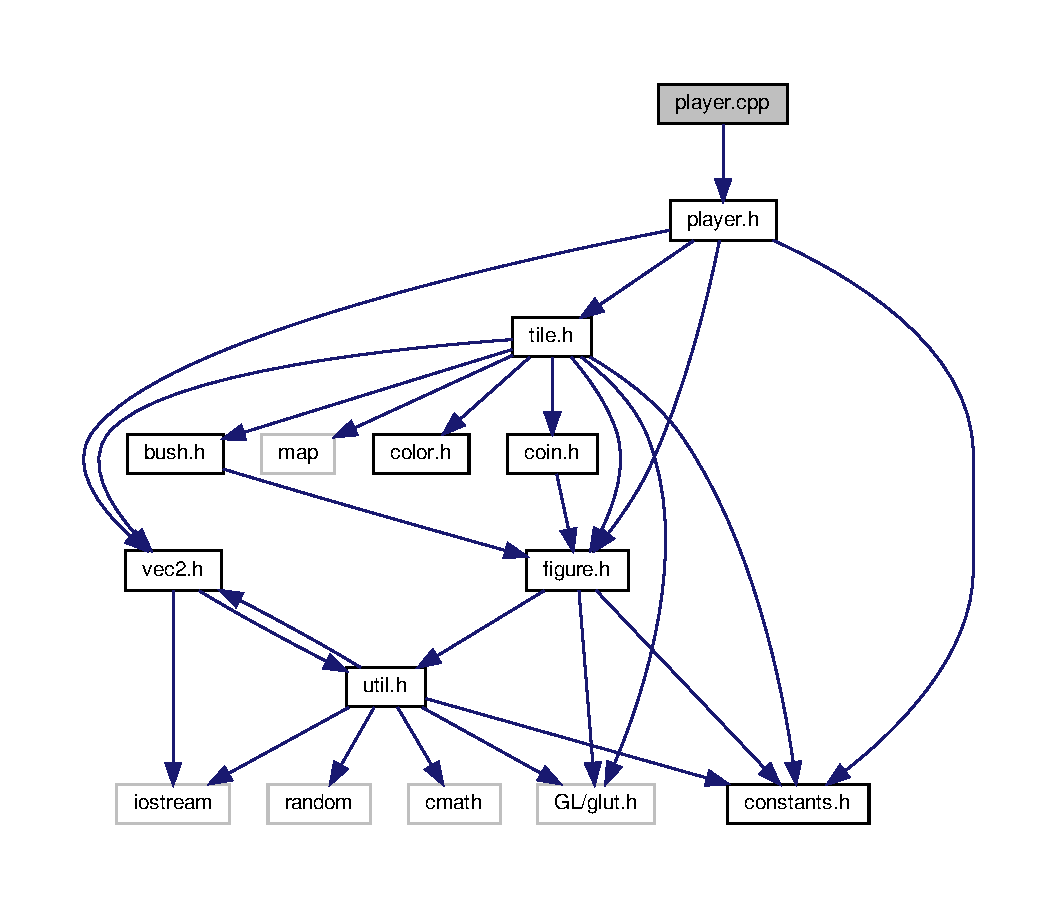
\includegraphics[width=350pt]{d5/d60/player_8cpp__incl}
\end{center}
\end{figure}

\hypertarget{player_8h}{}\section{player.\+h File Reference}
\label{player_8h}\index{player.\+h@{player.\+h}}
{\ttfamily \#include \char`\"{}constants.\+h\char`\"{}}\newline
{\ttfamily \#include \char`\"{}vec2.\+h\char`\"{}}\newline
{\ttfamily \#include \char`\"{}figure.\+h\char`\"{}}\newline
{\ttfamily \#include \char`\"{}tile.\+h\char`\"{}}\newline
Include dependency graph for player.\+h\+:
\nopagebreak
\begin{figure}[H]
\begin{center}
\leavevmode
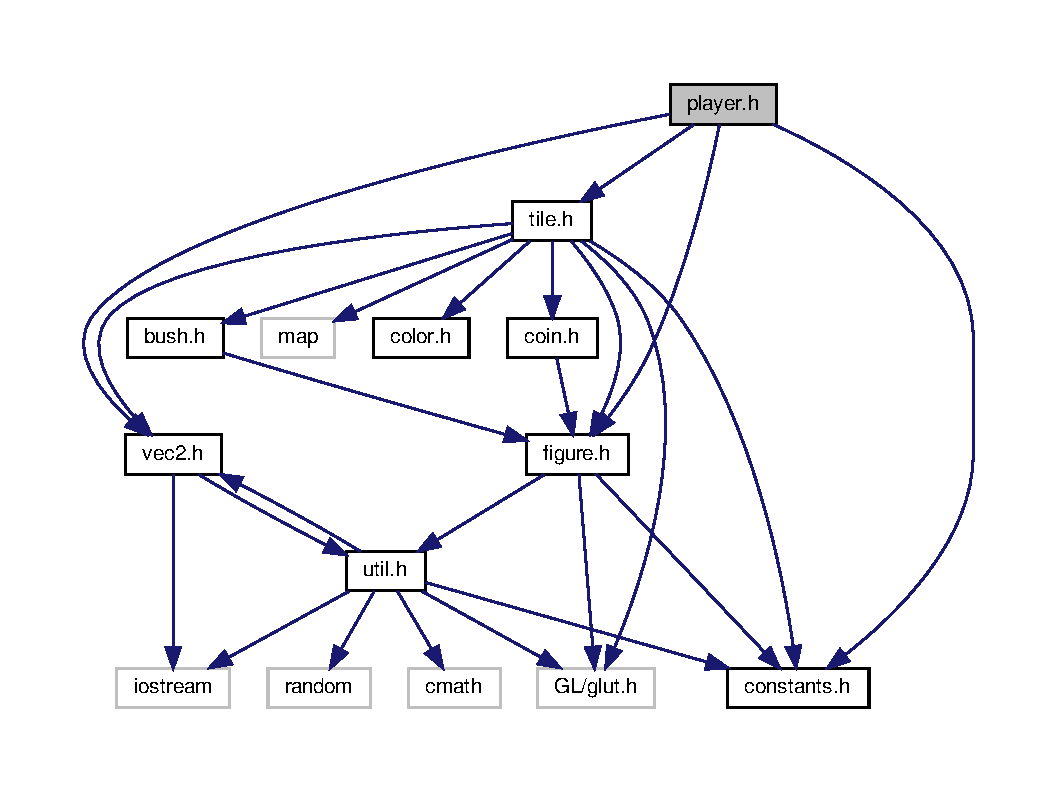
\includegraphics[width=350pt]{d1/d98/player_8h__incl}
\end{center}
\end{figure}
This graph shows which files directly or indirectly include this file\+:
\nopagebreak
\begin{figure}[H]
\begin{center}
\leavevmode
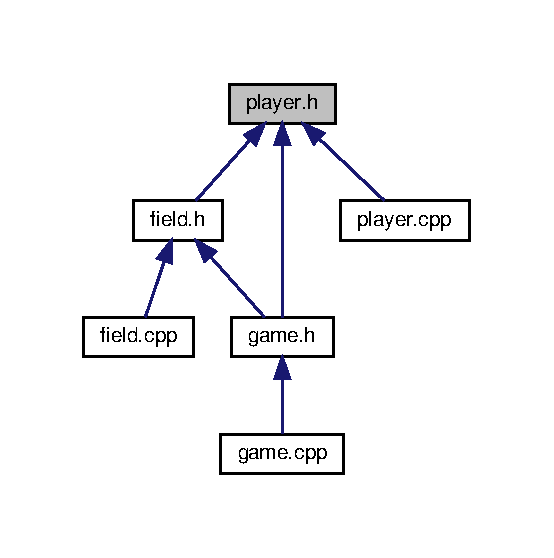
\includegraphics[width=266pt]{d9/d2f/player_8h__dep__incl}
\end{center}
\end{figure}
\subsection*{Classes}
\begin{DoxyCompactItemize}
\item 
class \hyperlink{classPlayer}{Player}
\end{DoxyCompactItemize}

\hypertarget{tile_8cpp}{}\section{tile.\+cpp File Reference}
\label{tile_8cpp}\index{tile.\+cpp@{tile.\+cpp}}
{\ttfamily \#include \char`\"{}tile.\+h\char`\"{}}\newline
Include dependency graph for tile.\+cpp\+:
\nopagebreak
\begin{figure}[H]
\begin{center}
\leavevmode
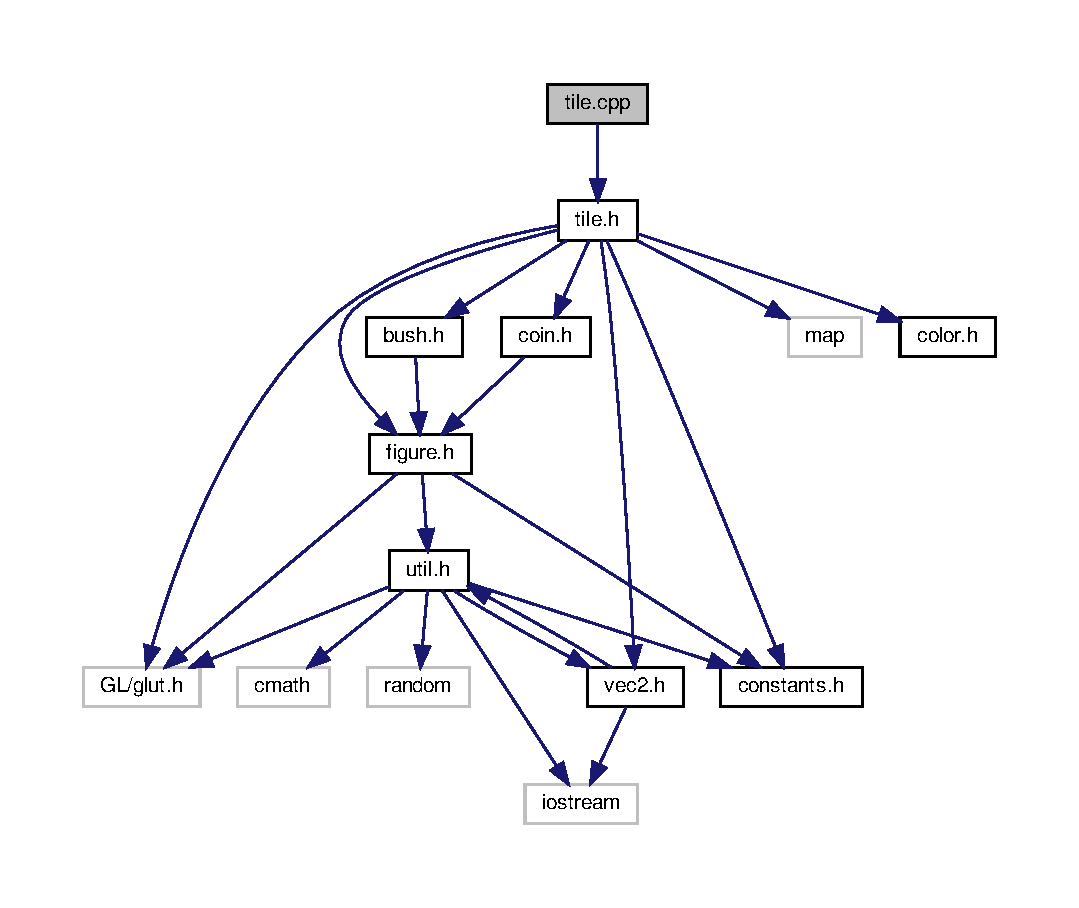
\includegraphics[width=350pt]{df/d9a/tile_8cpp__incl}
\end{center}
\end{figure}

\hypertarget{tile_8h}{}\section{tile.\+h File Reference}
\label{tile_8h}\index{tile.\+h@{tile.\+h}}
{\ttfamily \#include $<$G\+L/glut.\+h$>$}\newline
{\ttfamily \#include $<$map$>$}\newline
{\ttfamily \#include \char`\"{}color.\+h\char`\"{}}\newline
{\ttfamily \#include \char`\"{}figure.\+h\char`\"{}}\newline
{\ttfamily \#include \char`\"{}bush.\+h\char`\"{}}\newline
{\ttfamily \#include \char`\"{}coin.\+h\char`\"{}}\newline
{\ttfamily \#include \char`\"{}vec2.\+h\char`\"{}}\newline
{\ttfamily \#include \char`\"{}constants.\+h\char`\"{}}\newline
Include dependency graph for tile.\+h\+:
\nopagebreak
\begin{figure}[H]
\begin{center}
\leavevmode
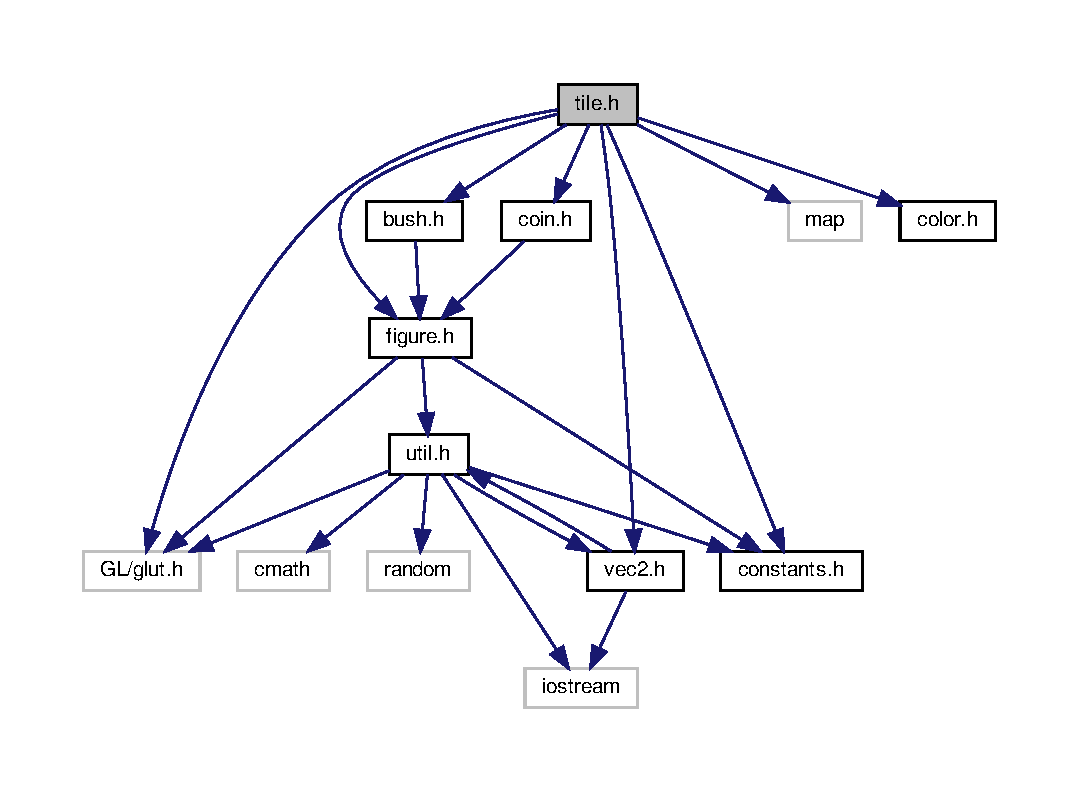
\includegraphics[width=350pt]{d0/d28/tile_8h__incl}
\end{center}
\end{figure}
This graph shows which files directly or indirectly include this file\+:
\nopagebreak
\begin{figure}[H]
\begin{center}
\leavevmode
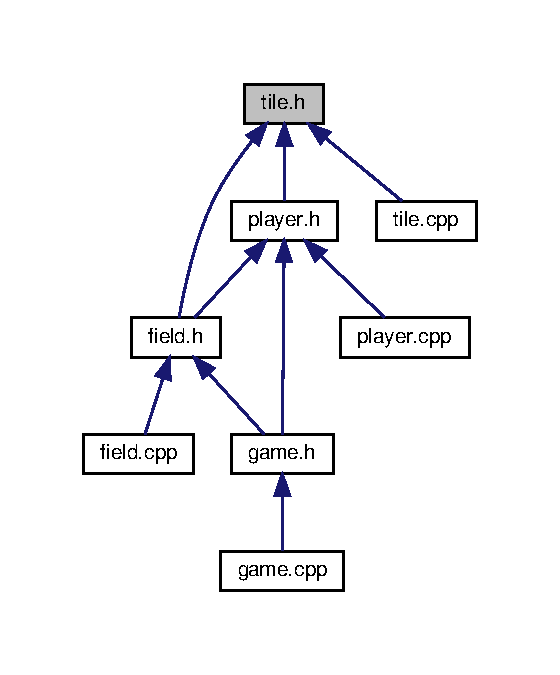
\includegraphics[width=299pt]{d3/d4a/tile_8h__dep__incl}
\end{center}
\end{figure}
\subsection*{Classes}
\begin{DoxyCompactItemize}
\item 
class \hyperlink{classTile}{Tile}
\end{DoxyCompactItemize}

\hypertarget{util_8cpp}{}\section{util.\+cpp File Reference}
\label{util_8cpp}\index{util.\+cpp@{util.\+cpp}}
{\ttfamily \#include \char`\"{}util.\+h\char`\"{}}\newline
Include dependency graph for util.\+cpp\+:
\nopagebreak
\begin{figure}[H]
\begin{center}
\leavevmode
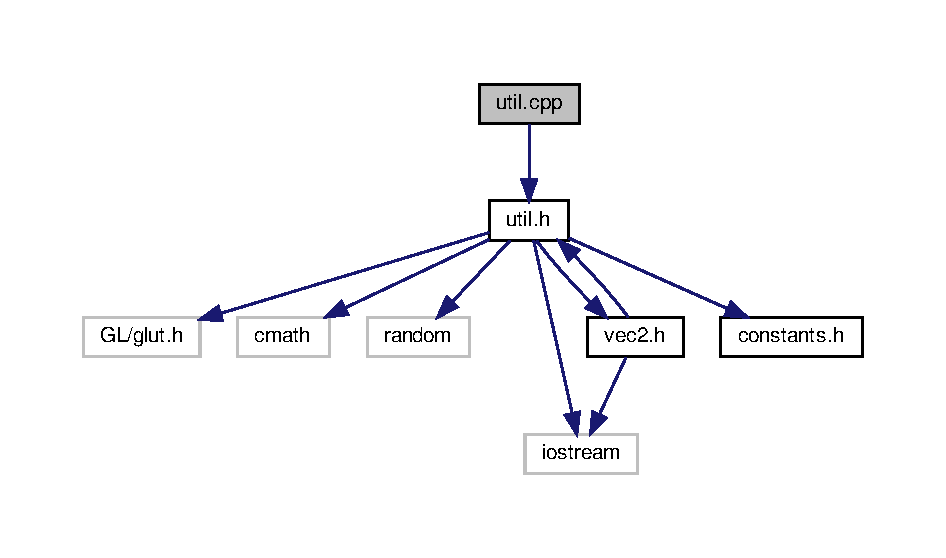
\includegraphics[width=350pt]{dd/d53/util_8cpp__incl}
\end{center}
\end{figure}
\subsection*{Functions}
\begin{DoxyCompactItemize}
\item 
float \hyperlink{util_8cpp_a4316695789dd880a5f5cd7af87c232b2}{randf} ()
\item 
\hyperlink{structvec2}{vec2} \hyperlink{util_8cpp_a0b9428f30ba2fc2753f3ba14da359f74}{get\+Hex\+Corner} (int n)
\item 
float \hyperlink{util_8cpp_a58b8858556ba861f0003021fdd94f5a3}{area\+Of\+Hexagon} (float radius)
\end{DoxyCompactItemize}


\subsection{Function Documentation}
\mbox{\Hypertarget{util_8cpp_a58b8858556ba861f0003021fdd94f5a3}\label{util_8cpp_a58b8858556ba861f0003021fdd94f5a3}} 
\index{util.\+cpp@{util.\+cpp}!area\+Of\+Hexagon@{area\+Of\+Hexagon}}
\index{area\+Of\+Hexagon@{area\+Of\+Hexagon}!util.\+cpp@{util.\+cpp}}
\subsubsection{\texorpdfstring{area\+Of\+Hexagon()}{areaOfHexagon()}}
{\footnotesize\ttfamily float area\+Of\+Hexagon (\begin{DoxyParamCaption}\item[{float}]{radius }\end{DoxyParamCaption})}

\mbox{\Hypertarget{util_8cpp_a0b9428f30ba2fc2753f3ba14da359f74}\label{util_8cpp_a0b9428f30ba2fc2753f3ba14da359f74}} 
\index{util.\+cpp@{util.\+cpp}!get\+Hex\+Corner@{get\+Hex\+Corner}}
\index{get\+Hex\+Corner@{get\+Hex\+Corner}!util.\+cpp@{util.\+cpp}}
\subsubsection{\texorpdfstring{get\+Hex\+Corner()}{getHexCorner()}}
{\footnotesize\ttfamily \hyperlink{structvec2}{vec2} get\+Hex\+Corner (\begin{DoxyParamCaption}\item[{int}]{n }\end{DoxyParamCaption})}

\mbox{\Hypertarget{util_8cpp_a4316695789dd880a5f5cd7af87c232b2}\label{util_8cpp_a4316695789dd880a5f5cd7af87c232b2}} 
\index{util.\+cpp@{util.\+cpp}!randf@{randf}}
\index{randf@{randf}!util.\+cpp@{util.\+cpp}}
\subsubsection{\texorpdfstring{randf()}{randf()}}
{\footnotesize\ttfamily float randf (\begin{DoxyParamCaption}{ }\end{DoxyParamCaption})}


\hypertarget{util_8h}{}\section{util.\+h File Reference}
\label{util_8h}\index{util.\+h@{util.\+h}}
{\ttfamily \#include $<$G\+L/glut.\+h$>$}\newline
{\ttfamily \#include $<$cmath$>$}\newline
{\ttfamily \#include $<$random$>$}\newline
{\ttfamily \#include $<$iostream$>$}\newline
{\ttfamily \#include \char`\"{}vec2.\+h\char`\"{}}\newline
{\ttfamily \#include \char`\"{}constants.\+h\char`\"{}}\newline
Include dependency graph for util.\+h\+:
\nopagebreak
\begin{figure}[H]
\begin{center}
\leavevmode
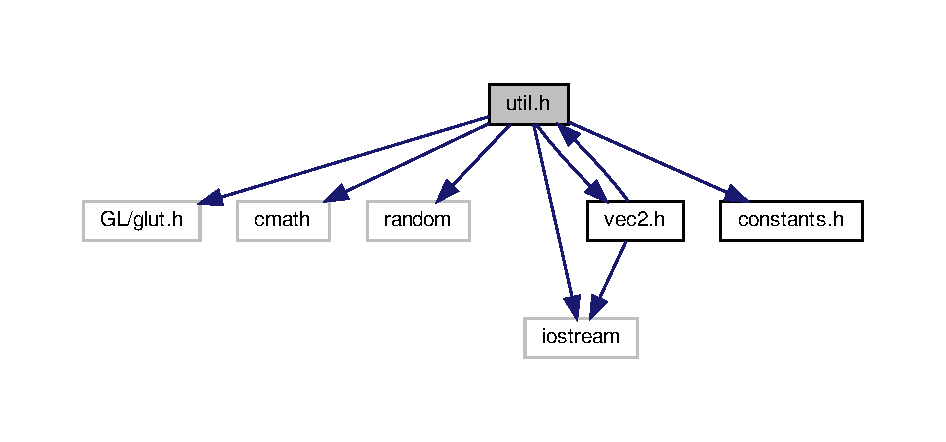
\includegraphics[width=350pt]{da/dee/util_8h__incl}
\end{center}
\end{figure}
This graph shows which files directly or indirectly include this file\+:
\nopagebreak
\begin{figure}[H]
\begin{center}
\leavevmode
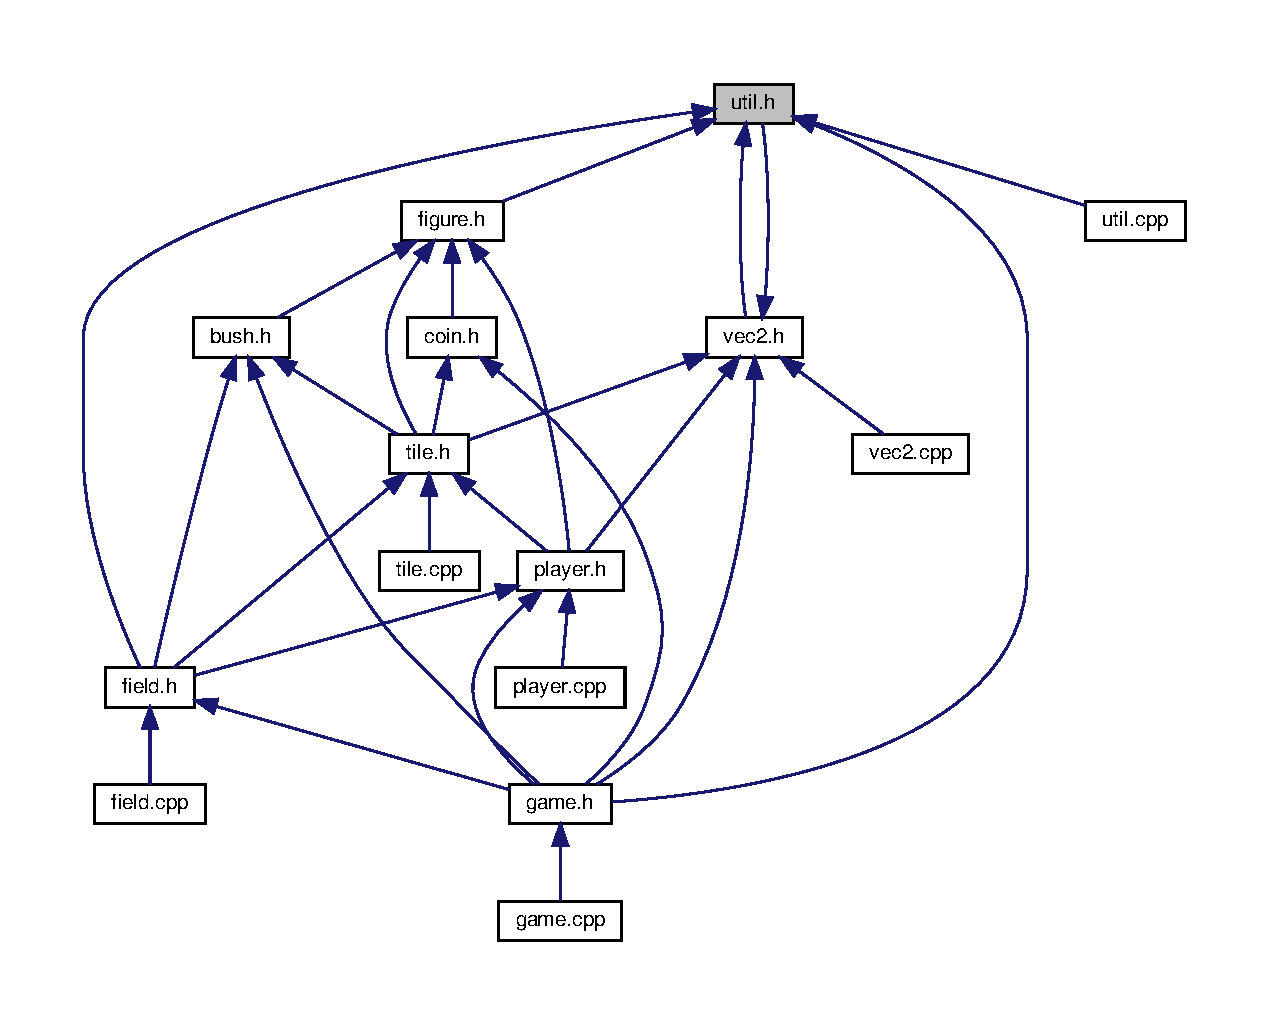
\includegraphics[width=350pt]{d6/de8/util_8h__dep__incl}
\end{center}
\end{figure}
\subsection*{Functions}
\begin{DoxyCompactItemize}
\item 
float \hyperlink{util_8h_a4316695789dd880a5f5cd7af87c232b2}{randf} ()
\item 
\hyperlink{structvec2}{vec2} \hyperlink{util_8h_a0b9428f30ba2fc2753f3ba14da359f74}{get\+Hex\+Corner} (int n)
\item 
float \hyperlink{util_8h_a58b8858556ba861f0003021fdd94f5a3}{area\+Of\+Hexagon} (float radius)
\end{DoxyCompactItemize}


\subsection{Function Documentation}
\mbox{\Hypertarget{util_8h_a58b8858556ba861f0003021fdd94f5a3}\label{util_8h_a58b8858556ba861f0003021fdd94f5a3}} 
\index{util.\+h@{util.\+h}!area\+Of\+Hexagon@{area\+Of\+Hexagon}}
\index{area\+Of\+Hexagon@{area\+Of\+Hexagon}!util.\+h@{util.\+h}}
\subsubsection{\texorpdfstring{area\+Of\+Hexagon()}{areaOfHexagon()}}
{\footnotesize\ttfamily float area\+Of\+Hexagon (\begin{DoxyParamCaption}\item[{float}]{radius }\end{DoxyParamCaption})}

\mbox{\Hypertarget{util_8h_a0b9428f30ba2fc2753f3ba14da359f74}\label{util_8h_a0b9428f30ba2fc2753f3ba14da359f74}} 
\index{util.\+h@{util.\+h}!get\+Hex\+Corner@{get\+Hex\+Corner}}
\index{get\+Hex\+Corner@{get\+Hex\+Corner}!util.\+h@{util.\+h}}
\subsubsection{\texorpdfstring{get\+Hex\+Corner()}{getHexCorner()}}
{\footnotesize\ttfamily \hyperlink{structvec2}{vec2} get\+Hex\+Corner (\begin{DoxyParamCaption}\item[{int}]{n }\end{DoxyParamCaption})}

\mbox{\Hypertarget{util_8h_a4316695789dd880a5f5cd7af87c232b2}\label{util_8h_a4316695789dd880a5f5cd7af87c232b2}} 
\index{util.\+h@{util.\+h}!randf@{randf}}
\index{randf@{randf}!util.\+h@{util.\+h}}
\subsubsection{\texorpdfstring{randf()}{randf()}}
{\footnotesize\ttfamily float randf (\begin{DoxyParamCaption}{ }\end{DoxyParamCaption})}


\hypertarget{vec2_8cpp}{}\section{vec2.\+cpp File Reference}
\label{vec2_8cpp}\index{vec2.\+cpp@{vec2.\+cpp}}
{\ttfamily \#include \char`\"{}vec2.\+h\char`\"{}}\newline
Include dependency graph for vec2.\+cpp\+:
\nopagebreak
\begin{figure}[H]
\begin{center}
\leavevmode
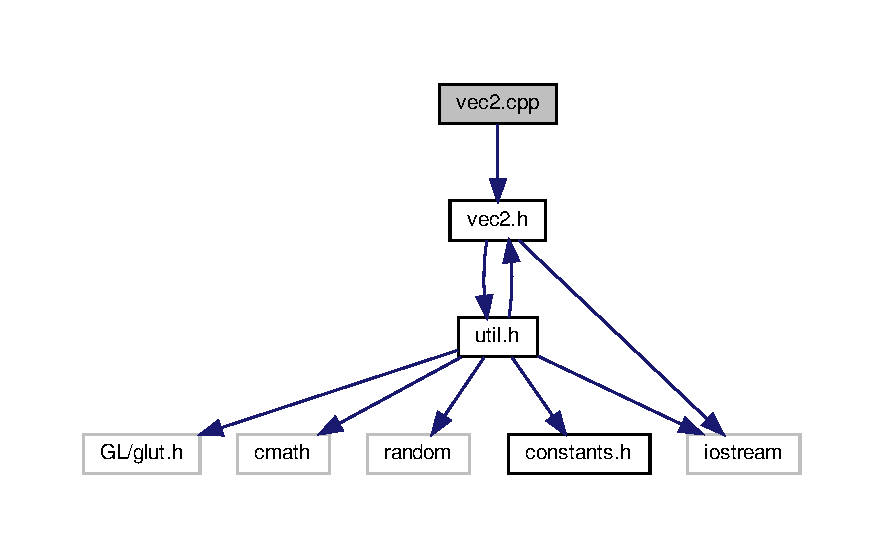
\includegraphics[width=350pt]{de/dde/vec2_8cpp__incl}
\end{center}
\end{figure}
\subsection*{Functions}
\begin{DoxyCompactItemize}
\item 
std\+::ostream \& \hyperlink{vec2_8cpp_a85b47f3582472fa5e3f80e6efd59f1d6}{operator$<$$<$} (std\+::ostream \&os, const \hyperlink{structvec2}{vec2} \&vec)
\end{DoxyCompactItemize}


\subsection{Function Documentation}
\mbox{\Hypertarget{vec2_8cpp_a85b47f3582472fa5e3f80e6efd59f1d6}\label{vec2_8cpp_a85b47f3582472fa5e3f80e6efd59f1d6}} 
\index{vec2.\+cpp@{vec2.\+cpp}!operator$<$$<$@{operator$<$$<$}}
\index{operator$<$$<$@{operator$<$$<$}!vec2.\+cpp@{vec2.\+cpp}}
\subsubsection{\texorpdfstring{operator$<$$<$()}{operator<<()}}
{\footnotesize\ttfamily std\+::ostream\& operator$<$$<$ (\begin{DoxyParamCaption}\item[{std\+::ostream \&}]{os,  }\item[{const \hyperlink{structvec2}{vec2} \&}]{vec }\end{DoxyParamCaption})}


\hypertarget{vec2_8h}{}\section{vec2.\+h File Reference}
\label{vec2_8h}\index{vec2.\+h@{vec2.\+h}}
{\ttfamily \#include \char`\"{}util.\+h\char`\"{}}\newline
{\ttfamily \#include $<$iostream$>$}\newline
Include dependency graph for vec2.\+h\+:
\nopagebreak
\begin{figure}[H]
\begin{center}
\leavevmode
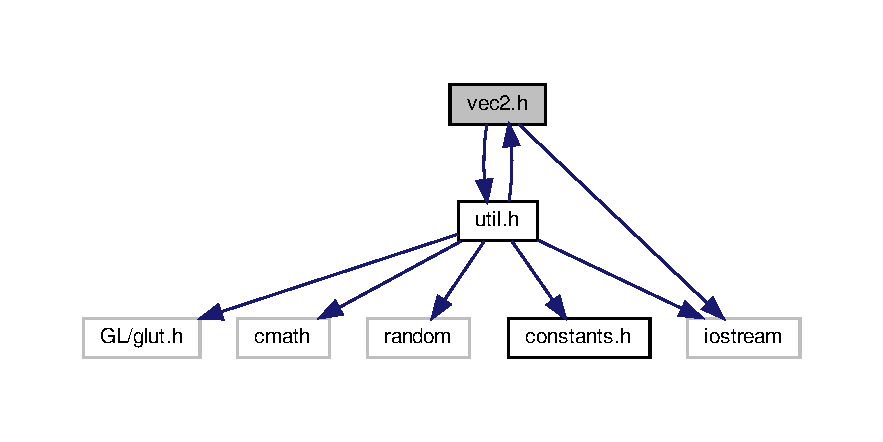
\includegraphics[width=350pt]{d5/dea/vec2_8h__incl}
\end{center}
\end{figure}
This graph shows which files directly or indirectly include this file\+:
\nopagebreak
\begin{figure}[H]
\begin{center}
\leavevmode
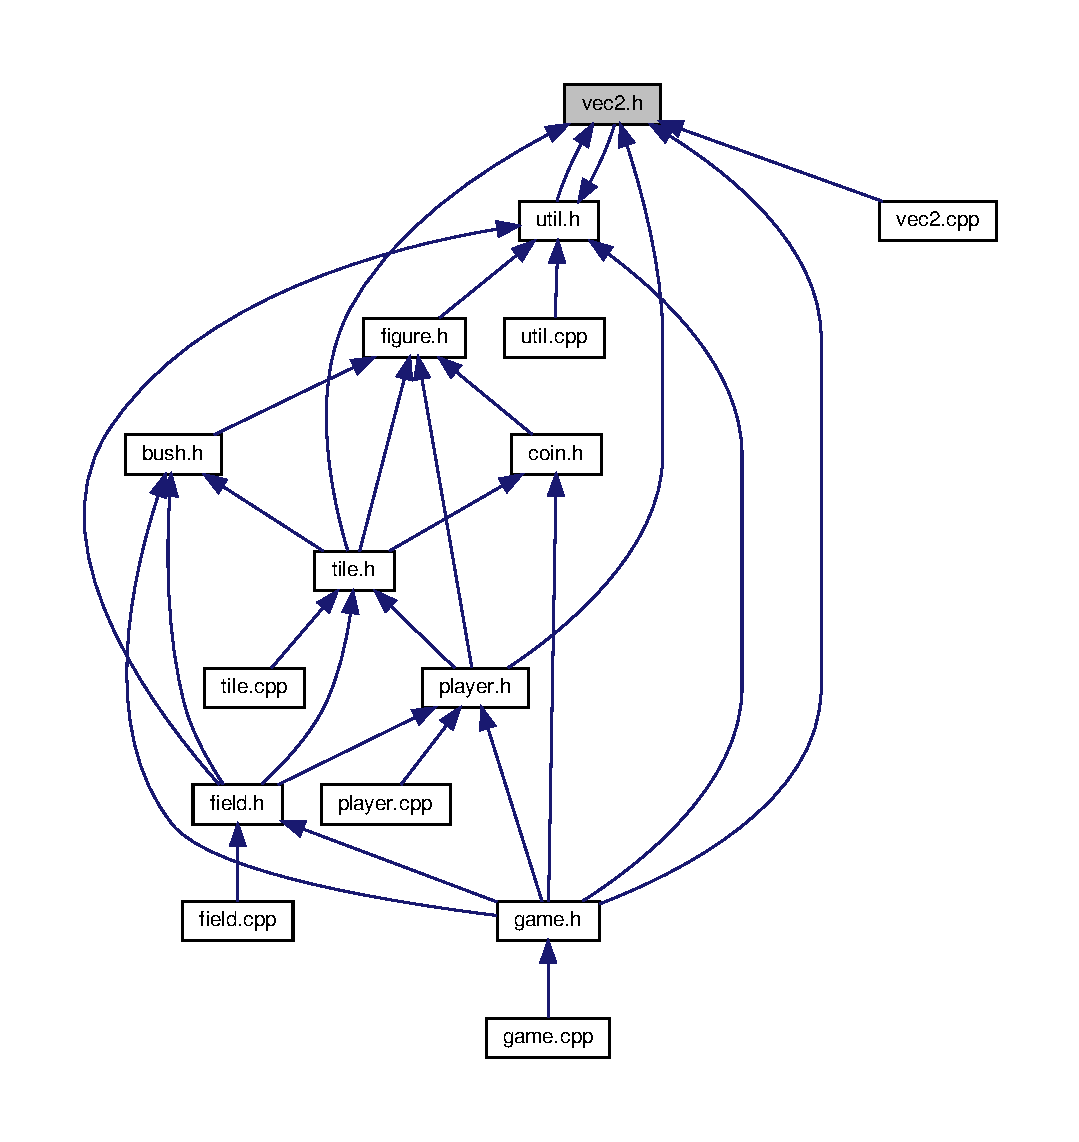
\includegraphics[width=350pt]{df/dd7/vec2_8h__dep__incl}
\end{center}
\end{figure}
\subsection*{Classes}
\begin{DoxyCompactItemize}
\item 
struct \hyperlink{structvec2}{vec2}
\end{DoxyCompactItemize}
\subsection*{Functions}
\begin{DoxyCompactItemize}
\item 
std\+::ostream \& \hyperlink{vec2_8h_a85b47f3582472fa5e3f80e6efd59f1d6}{operator$<$$<$} (std\+::ostream \&os, const \hyperlink{structvec2}{vec2} \&vec)
\end{DoxyCompactItemize}


\subsection{Function Documentation}
\mbox{\Hypertarget{vec2_8h_a85b47f3582472fa5e3f80e6efd59f1d6}\label{vec2_8h_a85b47f3582472fa5e3f80e6efd59f1d6}} 
\index{vec2.\+h@{vec2.\+h}!operator$<$$<$@{operator$<$$<$}}
\index{operator$<$$<$@{operator$<$$<$}!vec2.\+h@{vec2.\+h}}
\subsubsection{\texorpdfstring{operator$<$$<$()}{operator<<()}}
{\footnotesize\ttfamily std\+::ostream\& operator$<$$<$ (\begin{DoxyParamCaption}\item[{std\+::ostream \&}]{os,  }\item[{const \hyperlink{structvec2}{vec2} \&}]{vec }\end{DoxyParamCaption})}


%--- End generated contents ---

% Index
\backmatter
\newpage
\phantomsection
\clearemptydoublepage
\addcontentsline{toc}{chapter}{Index}
\printindex

\end{document}
